\documentclass[
twoside
% ,openany
,msc
,irfonts
,draft
]{./tex/tehran-thesis}

% در این فایل، دستورها و تنظیمات مورد نیاز، آورده شده است.
%-------------------------------------------------------------------------------------------------------------------
% دستوراتی که پوشه پیش‌فرض زیرفایل‌های tex را مشخص می‌کند.
%\makeatletter
%\def\input@path{{./tex/}}
%\makeatother
% در ورژن جدید زی‌پرشین برای تایپ متن‌های ریاضی، این سه بسته، حتماً باید فراخوانی شود
\usepackage{amsthm,amssymb,amsmath}
\usepackage{MnSymbol}
\usepackage{stmaryrd}
% بسته‌ای برای تنطیم حاشیه‌های بالا، پایین، چپ و راست صفحه
\usepackage[a4paper, top=40mm, bottom=40mm, outer=25mm, inner=35mm]{geometry}
% بسته‌‌ای برای ظاهر شدن شکل‌ها و تعیین آدرس تصاویر
\usepackage[final]{graphicx}
\graphicspath{{./img/}}
% بسته‌های مورد نیاز برای نوشتن کدها، رنگ‌آمیزی آنها و تعیین پوشهٔ کدها
\usepackage[final]{listings}
\usepackage[usenames,dvipsnames,svgnames,table]{xcolor}
\lstset{inputpath=./code/}
% بسته‌ای برای رسم کادر
\usepackage{framed} 
% بسته‌‌ای برای چاپ شدن خودکار تعداد صفحات در صفحه «معرفی پایان‌نامه»
\usepackage{lastpage}
% بسته‌ٔ لازم برای: ۱. تغییر شماره‌گذاری صفحات پیوست. ۲. تصحیح باگ آدرس وب حاوی '%' در مراجع
\usepackage{etoolbox}

%%%%%%%%%%%%%%%%%%%%%%%%%%%%%%%%%%%%
%%% دستورات وابسته به استیل مراجع:
%% اگر از استیل‌های natbib (plainnat-fa، asa-fa، chicago-fa) استفاده می‌کنید، خط زیر را فعال و بعدی‌اش را غیرفعال کنید.
%\usepackage{natbib}
%\newcommand{\citelatin}[1]{\cite{#1}\LTRfootnote{\citeauthor*{#1}}}
%\newcommand{\citeplatin}[1]{\citep{#1}\LTRfootnote{\citeauthor*{#1}}}
%% اگر از سایر استیل‌ها استفاده می‌کنید، خط بالا را غیرفعال و خط‌های زیر را فعال کنید.
\let\citep\cite
\let\citelatin\cite
\let\citeplatin\cite
%%%%%%%%%%%%
% بررسی حالت پیش نویس
\usepackage{ifdraft}
\ifdraft
{%
	% بسته‌ٔ ایجاد لینک‌های رنگی با امکان جهش
	\usepackage[unicode=true,pagebackref=true,
colorlinks,linkcolor=blue,citecolor=blue,final]{hyperref}
	%\usepackage{todonotes}
	\usepackage[firstpage]{draftwatermark}
	\SetWatermarkText{\ \ \ \rl{پیش‌نویس}}
	\SetWatermarkScale{1.2}
}
{ 
	\usepackage[pagebackref=false]{hyperref}
	%\usepackage[disable]{todonotes} % final without TODOs
}

\usepackage[obeyDraft]{todonotes}
\setlength{\marginparwidth}{2cm}

%%%%%%%%%%%%
%%% تصحیح باگ: اگر در مراجع، آدرس وب حاوی '%' بوده و pagebackref فعال باشد، دستورات زیر باید بیایند:
%% برای استیل‌های natbib مثل plainnat-fa، asa-fa، chicago-fa
\makeatletter
\let\ORIG@BR@@lbibitem\BR@@lbibitem
\apptocmd\ORIG@BR@@lbibitem{\endgroup}{}{}
\def\BR@@lbibitem{\begingroup\catcode`\%=12 \ORIG@BR@@lbibitem}
\makeatother
%% برای سایر استیل‌ها
\makeatletter
\let\ORIG@BR@@bibitem\BR@@bibitem
\apptocmd\ORIG@BR@@bibitem{\endgroup}{}{}
\def\BR@@bibitem{\begingroup\catcode`\%=12 \ORIG@BR@@bibitem}
\makeatother
%%%%%%%%%%%%%%%%%%%%%%%%%%%%%%%%%%%%

% بسته‌ لازم برای تنظیم سربرگ‌ها
\usepackage{fancyhdr}
%\usepackage{enumitem}
\usepackage{setspace}
% بسته‌های لازم برای نوشتن الگوریتم
\usepackage{algorithm}
\usepackage{algorithmic}
% بسته‌های لازم برای رسم بهتر جداول
\usepackage{tabulary}
\usepackage{tabularx}
\usepackage{rotating}
% بسته‌های لازم برای رسم تنظیم بهتر شکل‌ها و زیرشکل‌ها
\usepackage[export]{adjustbox}
\usepackage{subfig}
\usepackage[subfigure]{tocloft}
% بسته‌ای برای رسم نمودارها و نیز صفحه مالکیت اثر
\usepackage{tikz}
% بسته‌ای برای ظاهر شدن «مراجع» و «نمایه» در فهرست مطالب
\usepackage[nottoc]{tocbibind}
% دستورات مربوط به ایجاد نمایه
\usepackage{makeidx}
\makeindex
%%% بسته ایجاد واژه‌نامه با xindy
\usepackage[xindy,toc,acronym,nonumberlist=true]{glossaries}

% بسته‌ای برای افزودن تورفتگی به ابتدای اولین پاراگراف هر بخش
\usepackage{indentfirst}

% بسته زیر باگ ناشی از فراخوانی بسته‌های زیاد را برطرف می‌کند.
\usepackage{morewrites}
%%%%%%%%%%%%%%%%%%%%%%%%%%
% فراخوانی بسته زی‌پرشین (باید آخرین بسته باشد)
\usepackage[extrafootnotefeatures,  displaymathdigits=default]{xepersian}

\usepackage{import}

\makeatletter
% تعریف قلم فارسی و انگلیسی و مکان قلم‌ها
\if@irfonts
\settextfont[Path={./font/}, BoldFont={IRLotusICEE_Bold.ttf}, BoldItalicFont={IRLotusICEE_BoldIranic.ttf}, ItalicFont={IRLotusICEE_Iranic.ttf},Scale=1.2]{IRLotusICEE.ttf}
% LiberationSerif or FreeSerif as free equivalents of Times New Roman
\setlatintextfont[Path={./font/}, BoldFont={LiberationSerif-Bold.ttf}, BoldItalicFont={LiberationSerif-BoldItalic.ttf}, ItalicFont={LiberationSerif-Italic.ttf},Scale=1]{LiberationSerif-Regular.ttf}
% چنانچه می‌خواهید اعداد در فرمول‌ها، انگلیسی باشد، خط زیر را غیرفعال کنید
% و گزینهٔ displaymathdigits=persian را از خط ۱۰۹ حذف کنید.
\setdigitfont[Path={./font/}, Scale=1.2]{IRLotusICEE.ttf}
% تعریف قلم‌های فارسی و انگلیسی اضافی برای استفاده در بعضی از قسمت‌های متن
\setiranicfont[Path={./font/}, Scale=1.3]{IRLotusICEE_Iranic.ttf}				% ایرانیک، خوابیده به چپ
\setmathsfdigitfont[Path={./font/}]{IRTitr.ttf}
\defpersianfont\titlefont[Path={./font/}, Scale=1]{IRTitr.ttf}
% برای تعریف یک قلم خاص عنوان لاتین، خط بعد را فعال و ویرایش کنید و خط بعد از آن را غیرفعال کنید.
% \deflatinfont\latintitlefont[Scale=1]{LiberationSerif}
\font\latintitlefont=cmssbx10 scaled 2300 %cmssbx10 scaled 2300
\else
\settextfont{XB Niloofar}
\setlatintextfont{Junicode}
% چنانچه می‌خواهید اعداد در فرمول‌ها، انگلیسی باشد، خط زیر را غیرفعال کنید
% و گزینهٔ displaymathdigits=persian را از خط ۱۰۹ حذف کنید.
\setdigitfont{XB Niloofar}
% تعریف قلم‌های فارسی و انگلیسی اضافی برای استفاده در بعضی از قسمت‌های متن
% \setmathsfdigitfont{XB Titre}
\defpersianfont\titlefont{XB Titre}
\deflatinfont\latintitlefont[Scale=1.1]{Junicode}
\fi
\makeatother

% برای استفاده از قلم نستعلیق خط بعد را فعال کنید.
% \defpersianfont\nastaliq[Scale=1.2]{IranNastaliq}


%%%%%%%%%%%%%%%%%%%%%%%%%%
% راستچین شدن todonotes
\presetkeys{todonotes}{align=right,textdirection=righttoleft}{}
\makeatletter
\providecommand\@dotsep{5}
\def\listtodoname{فهرست کارهای باقیمانده}
\def\listoftodos{\noindent{\Large\vspace{10mm}\textbf{\listtodoname}}\@starttoc{tdo}}
\renewcommand{\@todonotes@MissingFigureText}{شکل}
\renewcommand{\@todonotes@MissingFigureUp}{شکل}
\renewcommand{\@todonotes@MissingFigureDown}{جاافتاده}
\makeatother
% دستوری برای حذف کلمه «چکیده»
% \renewcommand{\abstractname}{}
% دستوری برای حذف کلمه «abstract»
%\renewcommand{\latinabstract}{}
% دستوری برای تغییر نام کلمه «اثبات» به «برهان»
\renewcommand\proofname{\textbf{برهان}}
% دستوری برای تغییر نام کلمه «کتاب‌نامه» به «مراجع»
\renewcommand{\bibname}{مراجع}
% دستوری برای تعریف واژه‌نامه انگلیسی به فارسی
\newcommand\persiangloss[2]{#1\dotfill\lr{#2}\\}
% دستوری برای تعریف واژه‌نامه فارسی به انگلیسی 
\newcommand\englishgloss[2]{#2\dotfill\lr{#1}\\}
% تعریف دستور جدید «\پ» برای خلاصه‌نویسی جهت نوشتن عبارت «پروژه/پایان‌نامه/رساله»
\newcommand{\پ}{پروژه/پایان‌نامه/رساله }

%\newcommand\BackSlash{\char`\\}

%%%%%%%%%%%%%%%%%%%%%%%%%%
% \SepMark{-}

% تعریف و نحوه ظاهر شدن عنوان قضیه‌ها، تعریف‌ها، مثال‌ها و ...
\theoremstyle{definition}
\newtheorem{definition}{تعریف}[section]
\theoremstyle{theorem}
\newtheorem{theorem}[definition]{قضیه}
\newtheorem{lemma}[definition]{لم}
\newtheorem{proposition}[definition]{گزاره}
\newtheorem{corollary}[definition]{نتیجه}
\newtheorem{remark}[definition]{ملاحظه}
\theoremstyle{definition}
\newtheorem{example}[definition]{مثال}

%\renewcommand{\theequation}{\thechapter-\arabic{equation}}
%\def\bibname{مراجع}
\numberwithin{algorithm}{chapter}
\def\listalgorithmname{فهرست الگوریتم‌ها}
\def\listfigurename{فهرست تصاویر}
\def\listtablename{فهرست جداول}

% دستور های لازم برای تعریف ترجمهٔ دستورات الگوریتم
\makeatletter
\renewcommand{\algorithmicrequire}{\if@RTL\textbf{ورودی:}\else\textbf{Require:}\fi}
\renewcommand{\algorithmicensure}{\if@RTL\textbf{خروجی:}\else\textbf{Ensure:}\fi}
\renewcommand{\algorithmicend}{\if@RTL\textbf{پایان}\else\textbf{end}\fi}
\renewcommand{\algorithmicif}{\if@RTL\textbf{اگر}\else\textbf{if}\fi}
\renewcommand{\algorithmicthen}{\if@RTL\textbf{آنگاه}\else\textbf{then}\fi}
\renewcommand{\algorithmicelse}{\if@RTL\textbf{وگرنه}\else\textbf{else}\fi}
\renewcommand{\algorithmicfor}{\if@RTL\textbf{برای}\else\textbf{for}\fi}
\renewcommand{\algorithmicforall}{\if@RTL\textbf{برای هر}\else\textbf{for all}\fi}
\renewcommand{\algorithmicdo}{\if@RTL\textbf{انجام بده}\else\textbf{do}\fi}
\renewcommand{\algorithmicwhile}{\if@RTL\textbf{تا زمانی که}\else\textbf{while}\fi}
\renewcommand{\algorithmicloop}{\if@RTL\textbf{تکرار کن}\else\textbf{loop}\fi}
\renewcommand{\algorithmicrepeat}{\if@RTL\textbf{تکرار کن}\else\textbf{repeat}\fi}
\renewcommand{\algorithmicuntil}{\if@RTL\textbf{تا زمانی که}\else\textbf{until}\fi}
\renewcommand{\algorithmicprint}{\if@RTL\textbf{چاپ کن}\else\textbf{print}\fi}
\renewcommand{\algorithmicreturn}{\if@RTL\textbf{بازگردان}\else\textbf{return}\fi}
\renewcommand{\algorithmicand}{\if@RTL\textbf{و}\else\textbf{and}\fi}
\renewcommand{\algorithmicor}{\if@RTL\textbf{و یا}\else\textbf{or}\fi} % TODO add better translate
\renewcommand{\algorithmicxor}{\if@RTL\textbf{یا}\else\textbf{xor}\fi} % TODO add better translate
\renewcommand{\algorithmicnot}{\if@RTL\textbf{نقیض}\else\textbf{not}\fi}
\renewcommand{\algorithmicto}{\if@RTL\textbf{تا}\else\textbf{to}\fi}
\renewcommand{\algorithmicinputs}{\if@RTL\textbf{ورودی‌ها}\else\textbf{inputs}\fi}
\renewcommand{\algorithmicoutputs}{\if@RTL\textbf{خروجی‌ها}\else\textbf{outputs}\fi}
\renewcommand{\algorithmicglobals}{\if@RTL\textbf{متغیرهای عمومی}\else\textbf{globals}\fi}
\renewcommand{\algorithmicbody}{\if@RTL\textbf{انجام بده}\else\textbf{do}\fi}
\renewcommand{\algorithmictrue}{\if@RTL\textbf{درست}\else\textbf{true}\fi}
\renewcommand{\algorithmicfalse}{\if@RTL\textbf{نادرست}\else\textbf{false}\fi}
\renewcommand{\algorithmicendif}{\algorithmicend\textbf{ شرط }\algorithmicif}
\renewcommand{\algorithmicendfor}{\algorithmicend\textbf{ حلقهٔ }\algorithmicfor}
\renewcommand{\algorithmicendwhile}{\algorithmicend\textbf{ حلقهٔ }\algorithmicwhile}
\renewcommand{\algorithmicendloop}{\algorithmicend\textbf{ حلقهٔ }\algorithmicloop}
\renewcommand{\algorithmiccomment}[1]{\{{\itshape #1}\}}
\makeatletter

%%%%%%%%%%%%%%%%%%%%%%%%%%%%
%%% دستورهایی برای سفارشی کردن سربرگ صفحات:
%\newcommand{\SetHeader}[1]{
% دستور زیر معادل با گزینه twoside است.
%\csname@twosidetrue\endcsname
\pagestyle{fancy}
%% دستورات زیر سبک صفحات fancy را تغییر می‌دهد:
% O=Odd, E=Even, L=Left, R=Right
% در صورت oneside بودن، عنوان فصل، سمت چپ ظاهر می‌شود.
\fancyhead{}
\fancyhead[OL]{\small\leftmark}
\fancyhead[ER]{\small\leftmark}
\fancyhead[OR]{\footnotesize\rightmark}
\fancyhead[EL]{\footnotesize\rightmark}
\renewcommand{\headrulewidth}{0.75pt}
% شکل‌دهی شماره و عنوان فصل در سربرگ
\renewcommand{\chaptermark}[1]{\markboth{فصل~\thechapter:\ #1}{}}
\makeatletter
\renewcommand{\rightmark}[1]{\@title}
\makeatother
%}
%%%%%%%%%%%%%%%%%%%%%%%%%%%%
%\def\MATtextbaseline{1.5}
%\renewcommand{\baselinestretch}{\MATtextbaseline}
\doublespacing
%%%%%%%%%%%%%%%%%%%%%%%%%%%%%
% دستوراتی برای اضافه کردن کلمه «فصل» در فهرست مطالب

\newlength\mylenprt
\newlength\mylenchp
\newlength\mylenapp

\renewcommand\cftpartpresnum{\partname~}
\renewcommand\cftchappresnum{\chaptername~}
\renewcommand\cftchapaftersnum{:}

\settowidth\mylenprt{\cftpartfont\cftpartpresnum\cftpartaftersnum}
\settowidth\mylenchp{\cftchapfont\cftchappresnum\cftchapaftersnum}
\settowidth\mylenapp{\cftchapfont\appendixname~\cftchapaftersnum}
\addtolength\mylenprt{\cftpartnumwidth}
\addtolength\mylenchp{\cftchapnumwidth}
\addtolength\mylenapp{\cftchapnumwidth}

\setlength\cftpartnumwidth{\mylenprt}
\setlength\cftchapnumwidth{\mylenchp}	

\makeatletter
{\def\thebibliography#1{\chapter*{\refname\@mkboth
   {\uppercase{\refname}}{\uppercase{\refname}}}\list
   {[\arabic{enumi}]}{\settowidth\labelwidth{[#1]}
   \rightmargin\labelwidth
   \advance\rightmargin\labelsep
   \advance\rightmargin\bibindent
   \itemindent -\bibindent

   \listparindent \itemindent
   \parsep \z@
   \usecounter{enumi}}
   \def\newblock{}
   \sloppy
   \sfcode`\.=1000\relax}}
   
%اگر مایلید در شماره گذاری حرفی و ابجد به جای آ از الف استفاده شود دستورات زیر را فعال کنید.   
%\def\@Abjad#1{%
%  \ifcase#1\or الف\or ب\or ج\or د%
%           \or هـ\or و\or ز\or ح\or ط%
%           \or ی\or ک\or ل\or م\or ن%
%           \or س\or ع\or ف\or ص%
%           \or ق\or ر\or ش\or ت\or ث%
%            \or خ\or ذ\or ض\or ظ\or غ%
%            \else\@ctrerr\fi}
%
% \def\abj@num@i#1{%
%   \ifcase#1\or الف\or ب\or ج\or د%
%            \or هـ‍\or و\or ز\or ح\or ط\fi

%   \ifnum#1=\z@\abjad@zero\fi}   
%  
%   \def\@harfi#1{\ifcase#1\or الف\or ب\or پ\or ت\or ث\or

% ج\or چ\or ح\or خ\or د\or ذ\or ر\or ز\or ژ\or س\or ش\or ص\or ض\or ط\or ظ\or ع\or غ\or

% ف\or ق\or ک\or گ\or ل\or م\or ن\or و\or ه\or ی\else\@ctrerr\fi}

%
\makeatother

%%% امکان درج کد در سند
% در این قسمت رنگ، قلم و قالب‌بندی قسمت‌های مختلف یک کد تعیین می‌شود. 
\lstdefinestyle{myStyle}{
	basicstyle=\ttfamily, % whole listing /w verbatim font
	keywordstyle=\color{blue}\bfseries, % bold black keywords
	identifierstyle=, % nothing happens
	commentstyle=\color{LimeGreen}, % green comments
	stringstyle=\ttfamily\color{red}, % red typewriter font for strings
	showstringspaces=false % no special string spaces
	breaklines=true,
	breakatwhitespace=false,
	numbers=right, % line number formats
	numberstyle=\footnotesize\lr,
	numbersep=-10pt,
	frame=single,
	captionpos=b,
	captiondirection=RTL
}
\lstset{style=myStyle} % command to set default style
\def\lstlistingname{\rl{برنامهٔ}}
\def\lstlistlistingname{\rl{فهرست برنامه‌ها}}


% for numbering subsubsections
\setcounter{secnumdepth}{3}
%to include subsubsections in the table of contents
\setcounter{tocdepth}{3}

\makeatletter
\renewcommand{\p@subfigure}{\thefigure.}
\makeatother


\newcommand{\s}[1]{\{#1\}}
\newcommand{\sem}[1]{\llbracket #1 \rrbracket}
\newcommand{\his}[1]{\langle #1 \rangle}
\newcommand{\e}{\emptyset}
\newcommand{\la}{\leftarrow}
\newcommand{\ra}{\rightarrow}
\newcommand{\teq}{\triangleq}
\newcommand{\crd}[4][above]{
    \node[draw,circle,inner sep=2pt,fill,label={[#1]:#4}] at (#2,#3) {};
}


% !TeX root=../main.tex
\university{دانشگاه تهران}
\college{پردیس دانشکده‌های فنی}
\faculty{دانشکده مهندسی برق و کامپیوتر}
\department{}
\subject{مهندسی کامپیوتر}
\field{نرم‌افزار}
\title{توضیح خطا در شبکه‌های مبتنی بر نرم‌افزار با استفاده از استدلال مبتنی بر علیت}
\firstsupervisor{دکتر حسین حجت}
\firstsupervisorrank{استادیار}
% \secondsupervisor{دکتر محمدرضا موسوی}
% \secondsupervisorrank{استادیار}
\firstadvisor{دکتر محمدرضا موسوی}
\firstadvisorrank{استاد}
\internaljudge{}
\internaljudgerank{}
\externaljudge{}
\externaljudgerank{}
\externaljudgeuniversity{}
% نام نماینده کمیته تحصیلات تکمیلی در دانشکده \ گروه
\graduatedeputy{}
\graduatedeputyrank{}
% نام دانشجو را وارد کنید
\name{امیرحسین}
% نام خانوادگی دانشجو را وارد کنید
\surname{صیحانی}
% شماره دانشجویی دانشجو را وارد کنید
\studentID{810198198}
% تاریخ پایان‌نامه را وارد کنید
\thesisdate{شهریور ۱۴۰۱}
%\projectLabel{پایان‌نامه}

%\degree{}
%%%%%%%%%%%%%%%%%%%%%%%%%%%%%%%%%%%%%%%%%%%%%%%%%%%%
%% پایان‌نامه خود را تقدیم کنید! %%
\dedication
{
{\Large تقدیم به:}\\
\begin{flushleft}{
	\huge
	همسر و فرزندانم\\
	\vspace{7mm}
	و\\
	\vspace{7mm}
	پدر و مادرم
}
\end{flushleft}
}
\fa-abstract{
	جایگزینی شبکه‌های کامپیوتری سنتی با شبکه‌ها مبتنی بر نرم‌افزار%
\lf{Software-Defined Network}
باعث شده است تا استفاده از روش‌ها و ابزار‌های مبتنی بر روش‌های صوری%
\lf{Formal Methods}
برای درستی‌سنجی%
\lf{Verification}
این شبکه‌ها تسهیل شود.
با اینکه درستی‌سنجی لازمه‌ی رفع‌ایراد در سیستم‌ها است، اما پس از مشخص شدن وجود خطا در سیستم، پیدا کردن دلیل این مساله که چرا سیستم دچار خطا شده است همچنان بر عهده‌ی کاربر است و لازم است که او با تحلیل و بررسی سیستم علت مشکل را پیدا کند و ایراد سیستم را بر طرف کند.
ابزار‌های درستی‌سنجی در صورتی که سیستم مطابق انتظار رفتار نکند یک مثال‌نقض یا گواهی برای اثبات این موضوع به کاربر ارائه می‌کنند اما این مدارک به تنهایی و بدون پردازش بیشتر اطلاعات کافی از چرایی مشکل در اختیار نمی‌گذارند.

توضیح پدیده‌ها در متون فلسفه قرن‌ها مورد مطالعه قرار گرفته است و نتایج این مطالعات در قالب اصول استدلال مبتنی بر خلاف واقع%
\lf{Counterfactual Reasoning}
تجمیع شده است.
هالپرن%
\lf{Joseph Y. Halpern}
و پرل%
\lf{Judea Pearl}
یک فرمولاسیون ریاضی برای پیدا کردن علت واقعی%
\lf{Actual Cause}
بر اساس استدلال مبتنی بر خلاف واقع ارائه کرده‌اند که در پژوهش‌های متعددی برای ارائه توضیح در مورد خطای رخ داده در سیستم و پیدا کردن علت واقعی آن مورد استفاده قرار گرفته است.

در این پژوهش از مفهوم علت واقعی ارائه شده توسط هالپرن و پرل برای توضیح خطا در شبکه‌های مبتنی بر نرم‌افزار استفاده می‌شود.
به صورت دقیق‌تر در این پژوهش یک مدل علّی%
\lf{Casual Model}
ارائه می‌شود که با استفاده از آن می‌توان در مورد ساختارهای شبکه، مانند وجود هم‌روندی یا ترتیب میان به‌روز رسانی‌های شبکه، برای پیدا کردن علت واقعی رفتار نا امن شبکه استدلال کرد.

در این پژوهش برای توصیف نرم‌افزار شبکه از زبان نت‌کت‌ پویا%
\lf{DyNetKAT}
استفاده می‌شود.
نت‌کت پویا یک سطح‌ بالا برنامه‌ نویسی شبکه است که بر پایه نت‌کت%
\lf{NetKAT}
 بنا شده و با وجود اینکه مینیمال بودن آن را حفظ کرده امکان توصیف به‌روز رسانی‌های پویای شبکه را فراهم می‌کند.
در این پژوهش از ساختمان رویداد%
\lf{Event Structure}
به عنوان مدل معنایی%
\lf{Semantic Model}
برنامه‌های نت‌کت پویا استفاده می‌شود.
ساختمان رویداد امکان توصیف صریح هم‌روندی را فراهم می‌کند که این موضوع سبب می‌شود چنین روابطی میان پردازه‌ها را هم بتوان به عنوان علت خطا در نظر گرفت، امری که با استفاده از مدل‌های برگ‌برگ شده%
\lf{Interleaving}
امکان پذیر نیست.
روش ارائه شده در این پژوهش برای پیدا کردن علت نقض چند ویژگی مطرح 
شبکه، مثلا نبود دور، مورد استفاده قرار گرفته است و بررسی این مساله‌ها نشان می‌دهد که علت‌های پیدا شده با شهود موجود از علت خطا در سیستم تطابق دارند.

}
\keywords{استدلال مبتنی بر علیت، ساختمان رویداد، درستی‌سنجی،
 شبکه‌های مبتنی بر نرم‌افزار}

% !TeX root=../main.tex
% در این فایل، عنوان پایان‌نامه، مشخصات خود و چکیده پایان‌نامه را به انگلیسی، وارد کنید.

%%%%%%%%%%%%%%%%%%%%%%%%%%%%%%%%%%%%
\latinuniversity{University of Tehran}
\latincollege{College of Engineering}
\latinfaculty{Faculty of Electrical and Computer Engineering}
\latindepartment{}
\latinsubject{Computer Engineering}
\latinfield{Software Engineering}
\latintitle{Explaining Software-Defined Networks Failures using Causal Reasoning}
\firstlatinsupervisor{Dr. Hossein Hojjat}
\secondlatinsupervisor{Dr. Mohammad Reza Mousavi}
\firstlatinadvisor{First Advisor}
%\secondlatinadvisor{Second Advisor}
\latinname{Amir Hossein}
\latinsurname{Seyhani}
\latinthesisdate{September 2022}
\latinkeywords{Writing Thesis, Template, \LaTeX, \XePersian}
\en-abstract{
This thesis studies on writing projects, theses and dissertations using tehran-thesis class. It ...
}

%%% تنظیمات مربوط به بسته  glossaries
%%% تعریف استایل برای واژه‌نامه فارسی به انگلیسی، در این استایل واژه‌های فارسی در سمت راست و واژه‌های انگلیسی در سمت چپ خواهند آمد. از حالت گروه ‌بندی استفاده می‌کنیم، 
%%% یعنی واژه‌ها در گروه‌هایی به ترتیب حروف الفبا مرتب می‌شوند، مثلا:
%%% الف
%%% افتصاد ................................... Economy
%%% اشکال ........................................ Failure
%%% ش
%%% شبکه ...................................... Network
\newglossarystyle{myFaToEn}{%
	\renewenvironment{theglossary}{}{}
	\renewcommand*{\glsgroupskip}{\vskip 10mm}
	\renewcommand*{\glsgroupheading}[1]{\subsection*{\glsgetgrouptitle{##1}}}
	\renewcommand*{\glossentry}[2]{\noindent\glsentryname{##1}\dotfill\space \glsentrytext{##1}
		
	}
}

%% % تعریف استایل برای واژه‌نامه انگلیسی به فارسی، در این استایل واژه‌های فارسی در سمت راست و واژه‌های انگلیسی در سمت چپ خواهند آمد. از حالت گروه ‌بندی استفاده می‌کنیم، 
%% % یعنی واژه‌ها در گروه‌هایی به ترتیب حروف الفبا مرتب می‌شوند، مثلا:
%% % E
%%% Economy ............................... اقتصاد
%% % F
%% % Failure................................... اشکال
%% %N
%% % Network ................................. شبکه

\newglossarystyle{myEntoFa}{%
	%%% این دستور در حقیقت عملیات گروه‌بندی را انجام می‌دهد. بدین صورت که واژه‌ها در بخش‌های جداگانه گروه‌بندی می‌شوند، 
	%%% عنوان بخش همان نام حرفی است که هر واژه در آن گروه با آن شروع شده است. 
	\renewenvironment{theglossary}{}{}
	\renewcommand*{\glsgroupskip}{\vskip 10mm}
	\renewcommand*{\glsgroupheading}[1]{\begin{LTR} \subsection*{\glsgetgrouptitle{##1}} \end{LTR}}
	%%% در این دستور نحوه نمایش واژه‌ها می‌آید. در این جا واژه فارسی در سمت راست و واژه انگلیسی در سمت چپ قرار داده شده است، و بین آن با نقطه پر می‌شود. 
	\renewcommand*{\glossentry}[2]{\noindent\glsentrytext{##1}\dotfill\space \glsentryname{##1}
		
	}
}

%%% تعیین استایل برای فهرست اختصارات
\newglossarystyle{myAbbrlist}{%
	%%% این دستور در حقیقت عملیات گروه‌بندی را انجام می‌دهد. بدین صورت که اختصارات‌ در بخش‌های جداگانه گروه‌بندی می‌شوند، 
	%%% عنوان بخش همان نام حرفی است که هر اختصار در آن گروه با آن شروع شده است. 
	\renewenvironment{theglossary}{}{}
	\renewcommand*{\glsgroupskip}{\vskip 10mm}
	\renewcommand*{\glsgroupheading}[1]{\begin{LTR} \subsection*{\glsgetgrouptitle{##1}} \end{LTR}}
	%%% در این دستور نحوه نمایش اختصارات می‌آید. در این جا حالت کوچک اختصار در سمت چپ و حالت بزرگ در سمت راست قرار داده شده است، و بین آن با نقطه پر می‌شود. 
	\renewcommand*{\glossentry}[2]{\noindent\Glsentrylong{##1}\dotfill\space \glsentrytext{##1} 
		
	}
	%%% تغییر نام محیط abbreviation به فهرست اختصارات
	\renewcommand*{\acronymname}{\rl{فهرست اختصارات}}
}

%%% برای اجرا xindy بر روی فایل .tex و تولید واژه‌نامه‌ها و فهرست اختصارات و فهرست نمادها یکسری  فایل تعریف شده است.‌ Latex داده های مربوط به واژه‌نامه و .. را در این 
%%%  فایل‌ها نگهداری می‌کند. مهم‌ترین option‌ این قسمت این است که 
%%% عنوان واژه‌نامه‌ها و یا فهرست اختصارات و یا فهرست نمادها را می‌توانید در این‌جا مشخص کنید. 
%%% در این جا عباراتی مثل glg، gls، glo و ... پسوند فایل‌هایی است که برای xindy بکار می‌روند. 
\newglossary[glg]{english}{gls}{glo}{واژه‌نامهٔ انگلیسی به فارسی}
\newglossary[blg]{persian}{bls}{blo}{واژه‌نامهٔ فارسی به انگلیسی}
\makeglossaries
\glsdisablehyper
%%% تعاریف مربوط به تولید واژه‌نامه و فهرست اختصارات و فهرست نمادها
%%%  در این فایل یکسری دستورات عمومی برای وارد کردن واژه‌نامه آمده است.
%%%  به دلیل این‌که قرار است این دستورات پایه‌ای را بازنویسی کنیم در این‌جا تعریف می‌کنیم. 
\let\oldgls\gls
\let\oldglspl\glspl

\makeatletter

\renewrobustcmd*{\gls}{\@ifstar\@msgls\@mgls}
\newcommand*{\@mgls}[1] {\ifthenelse{\equal{\glsentrytype{#1}}{english}}{\oldgls{#1}\glsuseri{f-#1}}{\lr{\oldgls{#1}}}}
\newcommand*{\@msgls}[1]{\ifthenelse{\equal{\glsentrytype{#1}}{english}}{\glstext{#1}\glsuseri{f-#1}}{\lr{\glsentryname{#1}}}}

\renewrobustcmd*{\glspl}{\@ifstar\@msglspl\@mglspl}
\newcommand*{\@mglspl}[1] {\ifthenelse{\equal{\glsentrytype{#1}}{english}}{\oldglspl{#1}\glsuseri{f-#1}}{\oldglspl{#1}}}
\newcommand*{\@msglspl}[1]{\ifthenelse{\equal{\glsentrytype{#1}}{english}}{\glsplural{#1}\glsuseri{f-#1}}{\glsentryplural{#1}}}

\makeatother

\newcommand{\newword}[4]{
	\newglossaryentry{#1}     {type={english},name={\lr{#2}},plural={#4},text={#3},description={}}
	\newglossaryentry{f-#1} {type={persian},name={#3},text={\lr{#2}},description={}}
}

%%% بر طبق این دستور، در اولین باری که واژه مورد نظر از واژه‌نامه وارد شود، پاورقی زده می‌شود. 
\defglsentryfmt[english]{\glsgenentryfmt\ifglsused{\glslabel}{}{\LTRfootnote{\glsentryname{\glslabel}}}}

%%% بر طبق این دستور، در اولین باری که واژه مورد نظر از فهرست اختصارات وارد شود، پاورقی زده می‌شود. 
\defglsentryfmt[acronym]{\glsentryname{\glslabel}\ifglsused{\glslabel}{}{\footnote{\glsentrydesc{\glslabel}}}}


%%%%%% ============================================================================================================

%%============================ دستور برای قرار دادن فهرست اختصارات 
\newcommand{\printabbreviation}{
	%\cleardoublepage
	%\phantomsection
	\baselineskip=.75cm
	\setglossarystyle{myAbbrlist}
	%\begin{LTR}
		\Oldprintglossary[type=acronym]	
	%\end{LTR}
	\clearpage
}%

\newcommand{\printacronyms}{\printabbreviation}
%%% در این جا محیط هر دو واژه‌نامه را باز تعریف کرده ایم، تا اولا مشکل قرار دادن صفحه اضافی را حل کنیم، ثانیا عنوان واژه‌نامه ها را با دستور addcontentlist وارد فهرست مطالب کرده ایم.
\let\Oldprintglossary\printglossary
\renewcommand{\printglossary}{
	\let\appendix\relax
	%% تنظیم کننده فاصله بین خطوط در این قسمت
	\clearpage
	%\phantomsection
	%% این دستور موجب این می‌شود که واژه‌نامه‌ها در  حالت دو ستونی نوشته شود. 
	\twocolumn{}
	\setglossarystyle{myFaToEn}
	\Oldprintglossary[type=persian]
	\clearpage
	%\phantomsection
	\setglossarystyle{myEntoFa}
	\Oldprintglossary[type=english]	
	\onecolumn{}
}%
%%%%%%

%%%% A
\newword{Gloss}{Glossary}{واژه‌نامه}{واژه‌نامه‌ها}

\newword{Acronym}{Acronym}{اختصار}{اختصارات}

\newword{Description}{Description}{توصیف}{توصیف‌ها}

\newword{Draft}{Draft}{پیش‌نویس}{پیش‌نویس‌ها}

\newword{Absorption}{Absorption}{جذب}{جذب‌ها}

\newword{RandomVariable}{Random Variable}
{متغیر تصادفی}{متغیرهای تصادفی}

\newword{Action}{Action}
{کنش}{کنش‌ها}

\newword{Optimization}{Optimization}{بهینه‌سازی}{}



\newacronym{a}{$a$}{\rl{شتاب ($m/s^2$)}}
\newacronym{F}{$F$}{\rl{نیرو ($N$)}}


\begin{document}

\pagenumbering{adadi} % یک، دو، ...
% ابتدای درج صفحات مختلف
\coverPage
% بررسی حالت پیش‌نویس
\ifoptiondraft{}{% 
    % \besmPage
    % \titlePage
    % \davaranPage
%%%%%%%%%%%%%%%%%%%%%%%%%%%
    \esalatPage
    \mojavezPage
% چنانچه مایل به چاپ صفحات «تقدیم»، «نیایش» و «سپاس‌گزاری» در خروجی نیستید، خط‌های زیر را با گذاشتن ٪  در ابتدای آنها غیرفعال کنید.
    % \taghdimPage
    % \ghadrdaniPage
} % end ifoptiondraft
\abstractPage
% شروع درج فهرست‌ها
\newpage\cleardoublepage
\pagenumbering{harfi} % آ، ب، ...
\tableofcontents \clearpage
% بررسی حالت پیش‌نویس برای بقیه فهرست‌ها
\ifoptiondraft{
    % \listoftodos
}{%
    % \listoffigures \clearpage
    % \listoftables  \clearpage
    % \addcontentsline{toc}{chapter}{\listalgorithmname}
    % \listofalgorithms \clearpage
    % \addcontentsline{toc}{chapter}{\lstlistlistingname}
    % \lstlistoflistings \clearpage
    % \printacronyms
} % end ifoptiondraft

\pagestyle{fancy}
\pagenumbering{arabic} % 1, 2, ...

% % !TeX root=../main.tex

\chapter{مقدمه}
% دستور زیر باعث عدم‌نمایش شماره صفحه در اولین صفحهٔ این فصل می‌شود.
%\thispagestyle{empty}
\section{آشنایی با این راهنما}
حروف‌چینی پروژه کارشناسی، پایان‌نامه یا رساله یکی از موارد پرکاربرد استفاده از
\lr{\LaTeX}
و زی‌پرشین
\cite{Khalighi87xepersian}
است. یک پروژه، پایان‌نامه یا رساله، احتیاج به تنظیمات زیادی از نظر صفحه‌آرایی دارد که وقت زیادی از دانشجو می‌گیرد. به دلیل قابلیت‌های بسیار لاتک در حروف‌چینی، کلاسی با نام 
\lr{tehran-thesis}
برای حروف‌چینی پروژه‌ها، پایان‌نامه‌ها و رساله‌های دانشگاه تهران، بر مبنای کلاس مشابه
\lr{IUST-Thesis}
تهیه شده است. این کلاس و فایل‌های همراه آن به گونه‌ای طراحی شده است که مطابق با دستورالعمل نگارش و تدوین پایان‌نامه کارشناسی ارشد و دکتری پردیس دانشکده‌های فنی دانشگاه تهران
\cite{UTThesisGuide}
باشد.

دستورالعمل نگارش و تدوین پایان‌نامه دانشگاه تهران به دو مقوله می‌پردازد، اول قالب و چگونگی صفحه‌آرایی پایان‌نامه، مانند اندازه و نوع قلم بخشهای مختلف، چینش فصلها، قالب مراجع و مواردی از این قبیل و دوم محتوای هر فصل پایان‌نامه. 
درصورت استفاده از این کلاس، نیازی نیست که دانشجو نگران مقوله اول باشد و پس از تایپ مطالب خود می‌تواند آنها را با لاتک و ابزار آن اجرا کند تا پایان‌نامه خود را با قالب دانشگاه داشته باشد. همچنین با خواندن این راهنما از ملزومات محتوایی هر فصل پایان‌نامه نیز مطلع خواهد شد.

در ادامهٔ  مقدمهٔ این راهنما، ابتدا چگونگی استفاده از کلاس پایان‌نامه و فایل‌های همراه آن را به صورت فنی شرح می‌دهیم و سپس مطالبی را در مورد ویژگی‌های محتوایی فصل ۱ پایان‌نامه (یعنی مقدمه) خواهیم آورد.
بقیهٔ فصل‌های این راهنما، تنها خصوصیات محتوایی فصول مختلف پایان‌نامه را شرح خواهند داد. نهایتاً جهت یادآوری، در پیوست‌ها مطالبی دربارهٔ آشنایی با دستورات لاتک، مدیریت مراجع در لاتک و چگونگی رسم جداول، نمودارها و الگوریتم‌ها آورده خواهند شد.

\section{چگونگی استفاده از کلاس پایان‌نامه}
کلیه فایل‌های لازم برای حروف‌چینی با کلاس فوق، داخل پوشه‌ای به نام
\lr{tehran-thesis}
قرار داده شده است. توجه داشته باشید که برای استفاده از این کلاس باید فونت‌های
\lr{IRLotusICEE}
و
\lr{IRTitr}
را داشته باشید (که همراه با این کلاس هست و نیاز به نصب نیست).
قلم‌های
\lr{IRLotusICEE}
مستخرج از قلم‌های استاندارد
\lr{IRLotus}
شورای عالی اطلاع‌رسانی%
\footnote{
قلم‌های استاندارد
\lr{IRFonts}
از شورای عالی اطلاع‌رسانی، منطبق بر آخرین نسخه استاندارد یونیکد، استاندارد ملی ۶۲۱۹ و استاندارد
\lr{Adobe Glyph Naming}
هستند.
}
هستند که توسط دکتر بابایی‌زاده اصلاحاتی روی آنها صورت پذیرفته است: تبدیل صفر توپر به صفر توخالی (جهت تمایز بیشتر با نقطه) و اضافه شدن
\textit{\textbf{حالت توپر و ایرانیک توأم}}،
که این موارد در قلم‌های شورای عالی اطلاع‌رسانی وجود ندارد.

\subsection{این همه فایل؟!}
\label{muchFiles}
از آنجایی که یک پایان‌نامه یا رساله، یک نوشته بلند محسوب می‌شود، لذا اگر همه تنظیمات و مطالب پایان‌نامه را داخل یک فایل قرار بدهیم، باعث شلوغی و سردرگمی می‌شود. به همین خاطر، قسمت‌های مختلف پایان‌نامه یا رساله  داخل فایل‌های جداگانه قرار گرفته است. مثلاً تنظیمات پایه‌ای کلاس داخل فایل
\lr{tehran-thesis.cls}، 
قسمت مشخصات فارسی پایان‌نامه داخل 
\lr{faTitle.tex}،
مطالب فصل اول داخل 
\lr{chapter1.tex}
و تنظیمات قابل تغییر توسط کاربر داخل 
\lr{commands.tex}،
قرار داده شده است.
\textbf{
	فایل اصلی این مجموعه، فایل
	\lr{main.tex}
	می‌باشد.
}
% یعنی بعد از تغییر فایل‌های دیگر، برای دیدن نتیجه تغییرات، باید این فایل را اجرا کرد. بقیه فایل‌ها به این فایل، کمک می‌کنند تا بتوانیم خروجی کار را ببینیم.
اگر به فایل 
\lr{main.tex}
دقت کنید، متوجه می‌شوید که قسمت‌های مختلف پایان‌نامه، توسط دستورهایی مانند 
\lr{input}
و
\lr{include}
به فایل اصلی، یعنی 
\lr{main.tex}
معرفی شده‌اند.
با توجه به ساختار محتوایی دستورالعمل، در فایل
\lr{main.tex}
فرض شده که پایان‌نامه یا رساله شما، از ۵ فصل و تعدادی پیوست تشکیل شده است. با اینحال، شما می‌توانید به راحتی فصل‌ها و پیوست‌ها را با صلاحدید اساتید راهنما، کم و زیاد کنید. این کار، بسیار ساده است. فرض کنید بخواهید یک فصل دیگر هم به پایان‌نامه اضافه کنید. برای این کار، کافی است یک فایل با نام دلخواه مثلاً 
\lr{chapter6}
و با پسوند 
\lr{.tex}
بسازید و آن را داخل پوشه 
\lr{tehran-thesis}
قرار دهید و سپس این فایل را با دستور 
\verb!\include{chapter6}!
داخل فایل
\lr{main.tex}
 فراخوانی کنید.

\subsection{از کجا شروع کنم؟}
قبل از هر چیز، باید یک توزیع تِک مناسب مانند تک‌لایو
\lr{(TeXLive)}
را روی سیستم خود نصب کنید. تک‌لایو  را می‌توانید از 
 \href{http://www.tug.org/texlive}{سایت رسمی آن}%
\LTRfootnote{\lr{\url{http://www.tug.org/texlive}}}
 دانلود کنید یا مستقیماً از مخازن توزیع لینوکس خود بگیرید (مثلاً در اوبونتو با دستور
\LRE{\verb!sudo apt install texlive-full!}).
برای نصب تک‌لایو و اجرای اسناد زی‌پرشین می‌توانید از
\href{http://parsilatex.com/site/shop/}{دی‌وی‌دی مجموعه پارسی‌لاتک}%
\LTRfootnote{\lr{\url{http://parsilatex.com/site/shop/}}}
و فایل راهنمای موجود در آن هم کمک بگیرید.

برای تایپ و پردازش اسناد لاتک باید از یک ویرایشگر مناسب استفاده کنید. ویرایشگرهای
\lr{TeXWroks},
\lr{TeXstudio},
\lr{Texmaker}
و
\lr{BiDiTeXmaker}
بدین منظور تولید شده‌اند. می‌توان ویرایش‌گر 
 \href{https://bitbucket.org/srazi/biditexmaker3}{\lr{BiDiTeXmaker}}%
 \LTRfootnote{\lr{\url{https://bitbucket.org/srazi/biditexmaker3}}}
را که بویژه برای کار با زی‌پرشین و مطالب دوجهته بهبود یافته است، بهینه‌ترین ویرایشگر لاتک برای کار با اسناد فارسی عنوان کرد.
 
حال اگر نوشتن \پ اولین تجربه شما از کار با لاتک است، توصیه می‌شود که یک‌بار به صورت اجمالی، کتاب «%
\href{http://www.tug.ctan.org/tex-archive/info/lshort/persian/lshort.pdf}{مقدمه‌ای نه چندان کوتاه بر
\lr{\LaTeXe}}%
\LTRfootnote{\lr{\url{http://www.tug.ctan.org/tex-archive/info/lshort/persian/lshort.pdf}\hfill}}»
ترجمه دکتر مهدی امیدعلی را مطالعه کنید. این کتاب، کتاب بسیار کاملی است که خیلی از نیازهای شما در ارتباط با حروف‌چینی را برطرف می‌کند.
اگر تک لایو کامل را داشته باشید، این کتاب را هم دارید. کافیست در خط فرمان دستور زیر را بزنید:
\begin{latin}
	\texttt{texdoc lshort-persian}
\end{latin}
اگر عجله دارید، برخی دستورات پایه‌ای مورد نیاز در پیوست \ref{app:latexIntro} بیان شده‌اند.
 
بعد از موارد گفته شده، فایل 
\lr{main.tex}
و
\lr{faTitle.tex}
را باز کنید و مشخصات پایان‌نامه خود مثل نام، نام خانوادگی، عنوان پایان‌نامه و ... را جایگزین مشخصات موجود در فایل
\lr{faTitle.tex}
 کنید. نیازی نیست نگران چینش این مشخصات در فایل پی‌دی‌اف خروجی باشید، زیرا کلاس 
\lr{tehran-thesis}
همه این کارها را بطور خودکار برای شما انجام می‌دهد. در ضمن، موقع تغییر دادن دستورهای داخل فایل
\lr{faTitle.tex}
 کاملاً دقت کنید؛ این دستورها، خیلی حساس هستند و ممکن است با یک تغییر کوچک، موقع اجرا، خطا بگیرید. برای دیدن خروجی کار، فایل 
\lr{faTitle.tex}
 را 
\lr{Save}
(نه 
\lr{Save As})
کنید و بعد به فایل 
\lr{main.tex}
برگشته و آن را اجرا کنید%
\footnote{
	البته فایلهای این مجموعه به گونه‌ای هستند که در
	\lr{TeXWorks} یا
	\lr{TeXstudio}
	بدون بازگشت به فایل اصلی، می‌توانید سند خود را اجرا کنید.
}.
 حال اگر می‌خواهید مشخصات انگلیسی \پ را هم عوض کنید، فایل 
\lr{enTitle.tex}
را باز کنید و مشخصات داخلش را تغییر دهید.
%\RTLfootnote{
%برای نوشتن پروژه کارشناسی، نیازی به وارد کردن مشخصات انگلیسی پروژه نیست. بنابراین، این مشخصات بطور خودکار، نادیده گرفته می‌شود.
%}
در اینجا هم برای دیدن خروجی باید این فایل را ذخیره کرده، بعد به فایل 
\lr{main.tex}
برگشته و آن را اجرا کرد.

برای راحتی بیشتر، کلاس 
\lr{tehran-thesis.cls}
طوری طراحی شده است که کافی است فقط  یک‌بار مشخصات \پ را (در فایل‌های
\lr{faTitle.tex}
و
\lr{enTitle.tex})
وارد کنید و هر جای دیگر که این مشخصات لازم باشند، به طور خودکار درج می‌شوند. با این حال، اگر مایل بودید، می‌توانید تنظیمات موجود را تغییر دهید؛ گرچه، در صورتیکه کاربر مبتدی هستید و یا با ساختار فایل‌های  
\lr{cls}
 آشنایی ندارید، بهتر است به فایل 
\lr{tehran-thesis.cls}
دست نزنید.

نکته دیگری که باید به آن توجه کنید این است که در قالب آماده شده، سه گزینه به نام‌های
\lr{bsc}،
\lr{msc}
و
\lr{phd}
برای نوشتن پروژه، پایان‌نامه و رساله، در نظر گرفته شده است. بنابراین اگر قصد تایپ پروژهٔ کارشناسی، پایان‌نامهٔ کارشناسی ارشد یا رسالهٔ دکتری را دارید، به ترتیب باید از گزینه‌های
\lr{bsc}،
\lr{msc}
و
\lr{phd}
در فایل 
\lr{main.tex}
استفاده کنید. با انتخاب هر کدام از این گزینه‌ها، تنظیمات مربوط به آنها به طور خودکار، اعمال می‌شود.


\subsection[مطالب پایان‌نامه را چطور بنویسم؟]
{مطالب \پ را چطور بنویسم؟}
\subsubsection{نوشتن فصل‌ها}
همان‌طور که در بخش \ref{muchFiles} گفته شد برای جلوگیری از شلوغی، قسمت‌های مختلف \پ از جمله فصل‌ها، در فایل‌های جداگانه‌ای قرار داده شده‌اند. 
مثلاً اگر می‌خواهید مطالب فصل ۱ را تایپ کنید، باید فایل‌های 
\lr{main.tex}
و
\lr{chapter1.tex}
را باز کرده و مطالب خود را جایگزین محتویات داخل 
\lr{chapter1.tex}
نمایید. دقت شود که در ابتدای برخی فایلها دستوراتی نوشته شده است و از شما خواسته شده که آن دستورات را حذف نکنید.

%توجه کنید که همان‌طور که قبلاً هم گفته شد، تنها فایل قابل اجرا، 
%\lr{main.tex}
%است. لذا برای دیدن حاصل (خروجی) فایل خود، باید  
%\lr{chapter1.tex}
%را ذخیره کرده و سپس فایل 
%\lr{main.tex}
%را اجرا کنید.

نکته بسیار مهمی که در اینجا باید گفته شود این است که سیستم \lr{\TeX}، محتویات یک فایل تِک را به ترتیب پردازش می‌کند.  بنابراین، اگر مثلاً  دو فصل اول خود را نوشته و خروجی آنها را دیده‌اید و مشغول تایپ مطالب فصل ۳ هستید، بهتر است
که دو دستور 
\verb!% !TeX root=../main.tex

\chapter{مقدمه}
% دستور زیر باعث عدم‌نمایش شماره صفحه در اولین صفحهٔ این فصل می‌شود.
%\thispagestyle{empty}
\section{آشنایی با این راهنما}
حروف‌چینی پروژه کارشناسی، پایان‌نامه یا رساله یکی از موارد پرکاربرد استفاده از
\lr{\LaTeX}
و زی‌پرشین
\cite{Khalighi87xepersian}
است. یک پروژه، پایان‌نامه یا رساله، احتیاج به تنظیمات زیادی از نظر صفحه‌آرایی دارد که وقت زیادی از دانشجو می‌گیرد. به دلیل قابلیت‌های بسیار لاتک در حروف‌چینی، کلاسی با نام 
\lr{tehran-thesis}
برای حروف‌چینی پروژه‌ها، پایان‌نامه‌ها و رساله‌های دانشگاه تهران، بر مبنای کلاس مشابه
\lr{IUST-Thesis}
تهیه شده است. این کلاس و فایل‌های همراه آن به گونه‌ای طراحی شده است که مطابق با دستورالعمل نگارش و تدوین پایان‌نامه کارشناسی ارشد و دکتری پردیس دانشکده‌های فنی دانشگاه تهران
\cite{UTThesisGuide}
باشد.

دستورالعمل نگارش و تدوین پایان‌نامه دانشگاه تهران به دو مقوله می‌پردازد، اول قالب و چگونگی صفحه‌آرایی پایان‌نامه، مانند اندازه و نوع قلم بخشهای مختلف، چینش فصلها، قالب مراجع و مواردی از این قبیل و دوم محتوای هر فصل پایان‌نامه. 
درصورت استفاده از این کلاس، نیازی نیست که دانشجو نگران مقوله اول باشد و پس از تایپ مطالب خود می‌تواند آنها را با لاتک و ابزار آن اجرا کند تا پایان‌نامه خود را با قالب دانشگاه داشته باشد. همچنین با خواندن این راهنما از ملزومات محتوایی هر فصل پایان‌نامه نیز مطلع خواهد شد.

در ادامهٔ  مقدمهٔ این راهنما، ابتدا چگونگی استفاده از کلاس پایان‌نامه و فایل‌های همراه آن را به صورت فنی شرح می‌دهیم و سپس مطالبی را در مورد ویژگی‌های محتوایی فصل ۱ پایان‌نامه (یعنی مقدمه) خواهیم آورد.
بقیهٔ فصل‌های این راهنما، تنها خصوصیات محتوایی فصول مختلف پایان‌نامه را شرح خواهند داد. نهایتاً جهت یادآوری، در پیوست‌ها مطالبی دربارهٔ آشنایی با دستورات لاتک، مدیریت مراجع در لاتک و چگونگی رسم جداول، نمودارها و الگوریتم‌ها آورده خواهند شد.

\section{چگونگی استفاده از کلاس پایان‌نامه}
کلیه فایل‌های لازم برای حروف‌چینی با کلاس فوق، داخل پوشه‌ای به نام
\lr{tehran-thesis}
قرار داده شده است. توجه داشته باشید که برای استفاده از این کلاس باید فونت‌های
\lr{IRLotusICEE}
و
\lr{IRTitr}
را داشته باشید (که همراه با این کلاس هست و نیاز به نصب نیست).
قلم‌های
\lr{IRLotusICEE}
مستخرج از قلم‌های استاندارد
\lr{IRLotus}
شورای عالی اطلاع‌رسانی%
\footnote{
قلم‌های استاندارد
\lr{IRFonts}
از شورای عالی اطلاع‌رسانی، منطبق بر آخرین نسخه استاندارد یونیکد، استاندارد ملی ۶۲۱۹ و استاندارد
\lr{Adobe Glyph Naming}
هستند.
}
هستند که توسط دکتر بابایی‌زاده اصلاحاتی روی آنها صورت پذیرفته است: تبدیل صفر توپر به صفر توخالی (جهت تمایز بیشتر با نقطه) و اضافه شدن
\textit{\textbf{حالت توپر و ایرانیک توأم}}،
که این موارد در قلم‌های شورای عالی اطلاع‌رسانی وجود ندارد.

\subsection{این همه فایل؟!}
\label{muchFiles}
از آنجایی که یک پایان‌نامه یا رساله، یک نوشته بلند محسوب می‌شود، لذا اگر همه تنظیمات و مطالب پایان‌نامه را داخل یک فایل قرار بدهیم، باعث شلوغی و سردرگمی می‌شود. به همین خاطر، قسمت‌های مختلف پایان‌نامه یا رساله  داخل فایل‌های جداگانه قرار گرفته است. مثلاً تنظیمات پایه‌ای کلاس داخل فایل
\lr{tehran-thesis.cls}، 
قسمت مشخصات فارسی پایان‌نامه داخل 
\lr{faTitle.tex}،
مطالب فصل اول داخل 
\lr{chapter1.tex}
و تنظیمات قابل تغییر توسط کاربر داخل 
\lr{commands.tex}،
قرار داده شده است.
\textbf{
	فایل اصلی این مجموعه، فایل
	\lr{main.tex}
	می‌باشد.
}
% یعنی بعد از تغییر فایل‌های دیگر، برای دیدن نتیجه تغییرات، باید این فایل را اجرا کرد. بقیه فایل‌ها به این فایل، کمک می‌کنند تا بتوانیم خروجی کار را ببینیم.
اگر به فایل 
\lr{main.tex}
دقت کنید، متوجه می‌شوید که قسمت‌های مختلف پایان‌نامه، توسط دستورهایی مانند 
\lr{input}
و
\lr{include}
به فایل اصلی، یعنی 
\lr{main.tex}
معرفی شده‌اند.
با توجه به ساختار محتوایی دستورالعمل، در فایل
\lr{main.tex}
فرض شده که پایان‌نامه یا رساله شما، از ۵ فصل و تعدادی پیوست تشکیل شده است. با اینحال، شما می‌توانید به راحتی فصل‌ها و پیوست‌ها را با صلاحدید اساتید راهنما، کم و زیاد کنید. این کار، بسیار ساده است. فرض کنید بخواهید یک فصل دیگر هم به پایان‌نامه اضافه کنید. برای این کار، کافی است یک فایل با نام دلخواه مثلاً 
\lr{chapter6}
و با پسوند 
\lr{.tex}
بسازید و آن را داخل پوشه 
\lr{tehran-thesis}
قرار دهید و سپس این فایل را با دستور 
\verb!\include{chapter6}!
داخل فایل
\lr{main.tex}
 فراخوانی کنید.

\subsection{از کجا شروع کنم؟}
قبل از هر چیز، باید یک توزیع تِک مناسب مانند تک‌لایو
\lr{(TeXLive)}
را روی سیستم خود نصب کنید. تک‌لایو  را می‌توانید از 
 \href{http://www.tug.org/texlive}{سایت رسمی آن}%
\LTRfootnote{\lr{\url{http://www.tug.org/texlive}}}
 دانلود کنید یا مستقیماً از مخازن توزیع لینوکس خود بگیرید (مثلاً در اوبونتو با دستور
\LRE{\verb!sudo apt install texlive-full!}).
برای نصب تک‌لایو و اجرای اسناد زی‌پرشین می‌توانید از
\href{http://parsilatex.com/site/shop/}{دی‌وی‌دی مجموعه پارسی‌لاتک}%
\LTRfootnote{\lr{\url{http://parsilatex.com/site/shop/}}}
و فایل راهنمای موجود در آن هم کمک بگیرید.

برای تایپ و پردازش اسناد لاتک باید از یک ویرایشگر مناسب استفاده کنید. ویرایشگرهای
\lr{TeXWroks},
\lr{TeXstudio},
\lr{Texmaker}
و
\lr{BiDiTeXmaker}
بدین منظور تولید شده‌اند. می‌توان ویرایش‌گر 
 \href{https://bitbucket.org/srazi/biditexmaker3}{\lr{BiDiTeXmaker}}%
 \LTRfootnote{\lr{\url{https://bitbucket.org/srazi/biditexmaker3}}}
را که بویژه برای کار با زی‌پرشین و مطالب دوجهته بهبود یافته است، بهینه‌ترین ویرایشگر لاتک برای کار با اسناد فارسی عنوان کرد.
 
حال اگر نوشتن \پ اولین تجربه شما از کار با لاتک است، توصیه می‌شود که یک‌بار به صورت اجمالی، کتاب «%
\href{http://www.tug.ctan.org/tex-archive/info/lshort/persian/lshort.pdf}{مقدمه‌ای نه چندان کوتاه بر
\lr{\LaTeXe}}%
\LTRfootnote{\lr{\url{http://www.tug.ctan.org/tex-archive/info/lshort/persian/lshort.pdf}\hfill}}»
ترجمه دکتر مهدی امیدعلی را مطالعه کنید. این کتاب، کتاب بسیار کاملی است که خیلی از نیازهای شما در ارتباط با حروف‌چینی را برطرف می‌کند.
اگر تک لایو کامل را داشته باشید، این کتاب را هم دارید. کافیست در خط فرمان دستور زیر را بزنید:
\begin{latin}
	\texttt{texdoc lshort-persian}
\end{latin}
اگر عجله دارید، برخی دستورات پایه‌ای مورد نیاز در پیوست \ref{app:latexIntro} بیان شده‌اند.
 
بعد از موارد گفته شده، فایل 
\lr{main.tex}
و
\lr{faTitle.tex}
را باز کنید و مشخصات پایان‌نامه خود مثل نام، نام خانوادگی، عنوان پایان‌نامه و ... را جایگزین مشخصات موجود در فایل
\lr{faTitle.tex}
 کنید. نیازی نیست نگران چینش این مشخصات در فایل پی‌دی‌اف خروجی باشید، زیرا کلاس 
\lr{tehran-thesis}
همه این کارها را بطور خودکار برای شما انجام می‌دهد. در ضمن، موقع تغییر دادن دستورهای داخل فایل
\lr{faTitle.tex}
 کاملاً دقت کنید؛ این دستورها، خیلی حساس هستند و ممکن است با یک تغییر کوچک، موقع اجرا، خطا بگیرید. برای دیدن خروجی کار، فایل 
\lr{faTitle.tex}
 را 
\lr{Save}
(نه 
\lr{Save As})
کنید و بعد به فایل 
\lr{main.tex}
برگشته و آن را اجرا کنید%
\footnote{
	البته فایلهای این مجموعه به گونه‌ای هستند که در
	\lr{TeXWorks} یا
	\lr{TeXstudio}
	بدون بازگشت به فایل اصلی، می‌توانید سند خود را اجرا کنید.
}.
 حال اگر می‌خواهید مشخصات انگلیسی \پ را هم عوض کنید، فایل 
\lr{enTitle.tex}
را باز کنید و مشخصات داخلش را تغییر دهید.
%\RTLfootnote{
%برای نوشتن پروژه کارشناسی، نیازی به وارد کردن مشخصات انگلیسی پروژه نیست. بنابراین، این مشخصات بطور خودکار، نادیده گرفته می‌شود.
%}
در اینجا هم برای دیدن خروجی باید این فایل را ذخیره کرده، بعد به فایل 
\lr{main.tex}
برگشته و آن را اجرا کرد.

برای راحتی بیشتر، کلاس 
\lr{tehran-thesis.cls}
طوری طراحی شده است که کافی است فقط  یک‌بار مشخصات \پ را (در فایل‌های
\lr{faTitle.tex}
و
\lr{enTitle.tex})
وارد کنید و هر جای دیگر که این مشخصات لازم باشند، به طور خودکار درج می‌شوند. با این حال، اگر مایل بودید، می‌توانید تنظیمات موجود را تغییر دهید؛ گرچه، در صورتیکه کاربر مبتدی هستید و یا با ساختار فایل‌های  
\lr{cls}
 آشنایی ندارید، بهتر است به فایل 
\lr{tehran-thesis.cls}
دست نزنید.

نکته دیگری که باید به آن توجه کنید این است که در قالب آماده شده، سه گزینه به نام‌های
\lr{bsc}،
\lr{msc}
و
\lr{phd}
برای نوشتن پروژه، پایان‌نامه و رساله، در نظر گرفته شده است. بنابراین اگر قصد تایپ پروژهٔ کارشناسی، پایان‌نامهٔ کارشناسی ارشد یا رسالهٔ دکتری را دارید، به ترتیب باید از گزینه‌های
\lr{bsc}،
\lr{msc}
و
\lr{phd}
در فایل 
\lr{main.tex}
استفاده کنید. با انتخاب هر کدام از این گزینه‌ها، تنظیمات مربوط به آنها به طور خودکار، اعمال می‌شود.


\subsection[مطالب پایان‌نامه را چطور بنویسم؟]
{مطالب \پ را چطور بنویسم؟}
\subsubsection{نوشتن فصل‌ها}
همان‌طور که در بخش \ref{muchFiles} گفته شد برای جلوگیری از شلوغی، قسمت‌های مختلف \پ از جمله فصل‌ها، در فایل‌های جداگانه‌ای قرار داده شده‌اند. 
مثلاً اگر می‌خواهید مطالب فصل ۱ را تایپ کنید، باید فایل‌های 
\lr{main.tex}
و
\lr{chapter1.tex}
را باز کرده و مطالب خود را جایگزین محتویات داخل 
\lr{chapter1.tex}
نمایید. دقت شود که در ابتدای برخی فایلها دستوراتی نوشته شده است و از شما خواسته شده که آن دستورات را حذف نکنید.

%توجه کنید که همان‌طور که قبلاً هم گفته شد، تنها فایل قابل اجرا، 
%\lr{main.tex}
%است. لذا برای دیدن حاصل (خروجی) فایل خود، باید  
%\lr{chapter1.tex}
%را ذخیره کرده و سپس فایل 
%\lr{main.tex}
%را اجرا کنید.

نکته بسیار مهمی که در اینجا باید گفته شود این است که سیستم \lr{\TeX}، محتویات یک فایل تِک را به ترتیب پردازش می‌کند.  بنابراین، اگر مثلاً  دو فصل اول خود را نوشته و خروجی آنها را دیده‌اید و مشغول تایپ مطالب فصل ۳ هستید، بهتر است
که دو دستور 
\verb!% !TeX root=../main.tex

\chapter{مقدمه}
% دستور زیر باعث عدم‌نمایش شماره صفحه در اولین صفحهٔ این فصل می‌شود.
%\thispagestyle{empty}
\section{آشنایی با این راهنما}
حروف‌چینی پروژه کارشناسی، پایان‌نامه یا رساله یکی از موارد پرکاربرد استفاده از
\lr{\LaTeX}
و زی‌پرشین
\cite{Khalighi87xepersian}
است. یک پروژه، پایان‌نامه یا رساله، احتیاج به تنظیمات زیادی از نظر صفحه‌آرایی دارد که وقت زیادی از دانشجو می‌گیرد. به دلیل قابلیت‌های بسیار لاتک در حروف‌چینی، کلاسی با نام 
\lr{tehran-thesis}
برای حروف‌چینی پروژه‌ها، پایان‌نامه‌ها و رساله‌های دانشگاه تهران، بر مبنای کلاس مشابه
\lr{IUST-Thesis}
تهیه شده است. این کلاس و فایل‌های همراه آن به گونه‌ای طراحی شده است که مطابق با دستورالعمل نگارش و تدوین پایان‌نامه کارشناسی ارشد و دکتری پردیس دانشکده‌های فنی دانشگاه تهران
\cite{UTThesisGuide}
باشد.

دستورالعمل نگارش و تدوین پایان‌نامه دانشگاه تهران به دو مقوله می‌پردازد، اول قالب و چگونگی صفحه‌آرایی پایان‌نامه، مانند اندازه و نوع قلم بخشهای مختلف، چینش فصلها، قالب مراجع و مواردی از این قبیل و دوم محتوای هر فصل پایان‌نامه. 
درصورت استفاده از این کلاس، نیازی نیست که دانشجو نگران مقوله اول باشد و پس از تایپ مطالب خود می‌تواند آنها را با لاتک و ابزار آن اجرا کند تا پایان‌نامه خود را با قالب دانشگاه داشته باشد. همچنین با خواندن این راهنما از ملزومات محتوایی هر فصل پایان‌نامه نیز مطلع خواهد شد.

در ادامهٔ  مقدمهٔ این راهنما، ابتدا چگونگی استفاده از کلاس پایان‌نامه و فایل‌های همراه آن را به صورت فنی شرح می‌دهیم و سپس مطالبی را در مورد ویژگی‌های محتوایی فصل ۱ پایان‌نامه (یعنی مقدمه) خواهیم آورد.
بقیهٔ فصل‌های این راهنما، تنها خصوصیات محتوایی فصول مختلف پایان‌نامه را شرح خواهند داد. نهایتاً جهت یادآوری، در پیوست‌ها مطالبی دربارهٔ آشنایی با دستورات لاتک، مدیریت مراجع در لاتک و چگونگی رسم جداول، نمودارها و الگوریتم‌ها آورده خواهند شد.

\section{چگونگی استفاده از کلاس پایان‌نامه}
کلیه فایل‌های لازم برای حروف‌چینی با کلاس فوق، داخل پوشه‌ای به نام
\lr{tehran-thesis}
قرار داده شده است. توجه داشته باشید که برای استفاده از این کلاس باید فونت‌های
\lr{IRLotusICEE}
و
\lr{IRTitr}
را داشته باشید (که همراه با این کلاس هست و نیاز به نصب نیست).
قلم‌های
\lr{IRLotusICEE}
مستخرج از قلم‌های استاندارد
\lr{IRLotus}
شورای عالی اطلاع‌رسانی%
\footnote{
قلم‌های استاندارد
\lr{IRFonts}
از شورای عالی اطلاع‌رسانی، منطبق بر آخرین نسخه استاندارد یونیکد، استاندارد ملی ۶۲۱۹ و استاندارد
\lr{Adobe Glyph Naming}
هستند.
}
هستند که توسط دکتر بابایی‌زاده اصلاحاتی روی آنها صورت پذیرفته است: تبدیل صفر توپر به صفر توخالی (جهت تمایز بیشتر با نقطه) و اضافه شدن
\textit{\textbf{حالت توپر و ایرانیک توأم}}،
که این موارد در قلم‌های شورای عالی اطلاع‌رسانی وجود ندارد.

\subsection{این همه فایل؟!}
\label{muchFiles}
از آنجایی که یک پایان‌نامه یا رساله، یک نوشته بلند محسوب می‌شود، لذا اگر همه تنظیمات و مطالب پایان‌نامه را داخل یک فایل قرار بدهیم، باعث شلوغی و سردرگمی می‌شود. به همین خاطر، قسمت‌های مختلف پایان‌نامه یا رساله  داخل فایل‌های جداگانه قرار گرفته است. مثلاً تنظیمات پایه‌ای کلاس داخل فایل
\lr{tehran-thesis.cls}، 
قسمت مشخصات فارسی پایان‌نامه داخل 
\lr{faTitle.tex}،
مطالب فصل اول داخل 
\lr{chapter1.tex}
و تنظیمات قابل تغییر توسط کاربر داخل 
\lr{commands.tex}،
قرار داده شده است.
\textbf{
	فایل اصلی این مجموعه، فایل
	\lr{main.tex}
	می‌باشد.
}
% یعنی بعد از تغییر فایل‌های دیگر، برای دیدن نتیجه تغییرات، باید این فایل را اجرا کرد. بقیه فایل‌ها به این فایل، کمک می‌کنند تا بتوانیم خروجی کار را ببینیم.
اگر به فایل 
\lr{main.tex}
دقت کنید، متوجه می‌شوید که قسمت‌های مختلف پایان‌نامه، توسط دستورهایی مانند 
\lr{input}
و
\lr{include}
به فایل اصلی، یعنی 
\lr{main.tex}
معرفی شده‌اند.
با توجه به ساختار محتوایی دستورالعمل، در فایل
\lr{main.tex}
فرض شده که پایان‌نامه یا رساله شما، از ۵ فصل و تعدادی پیوست تشکیل شده است. با اینحال، شما می‌توانید به راحتی فصل‌ها و پیوست‌ها را با صلاحدید اساتید راهنما، کم و زیاد کنید. این کار، بسیار ساده است. فرض کنید بخواهید یک فصل دیگر هم به پایان‌نامه اضافه کنید. برای این کار، کافی است یک فایل با نام دلخواه مثلاً 
\lr{chapter6}
و با پسوند 
\lr{.tex}
بسازید و آن را داخل پوشه 
\lr{tehran-thesis}
قرار دهید و سپس این فایل را با دستور 
\verb!\include{chapter6}!
داخل فایل
\lr{main.tex}
 فراخوانی کنید.

\subsection{از کجا شروع کنم؟}
قبل از هر چیز، باید یک توزیع تِک مناسب مانند تک‌لایو
\lr{(TeXLive)}
را روی سیستم خود نصب کنید. تک‌لایو  را می‌توانید از 
 \href{http://www.tug.org/texlive}{سایت رسمی آن}%
\LTRfootnote{\lr{\url{http://www.tug.org/texlive}}}
 دانلود کنید یا مستقیماً از مخازن توزیع لینوکس خود بگیرید (مثلاً در اوبونتو با دستور
\LRE{\verb!sudo apt install texlive-full!}).
برای نصب تک‌لایو و اجرای اسناد زی‌پرشین می‌توانید از
\href{http://parsilatex.com/site/shop/}{دی‌وی‌دی مجموعه پارسی‌لاتک}%
\LTRfootnote{\lr{\url{http://parsilatex.com/site/shop/}}}
و فایل راهنمای موجود در آن هم کمک بگیرید.

برای تایپ و پردازش اسناد لاتک باید از یک ویرایشگر مناسب استفاده کنید. ویرایشگرهای
\lr{TeXWroks},
\lr{TeXstudio},
\lr{Texmaker}
و
\lr{BiDiTeXmaker}
بدین منظور تولید شده‌اند. می‌توان ویرایش‌گر 
 \href{https://bitbucket.org/srazi/biditexmaker3}{\lr{BiDiTeXmaker}}%
 \LTRfootnote{\lr{\url{https://bitbucket.org/srazi/biditexmaker3}}}
را که بویژه برای کار با زی‌پرشین و مطالب دوجهته بهبود یافته است، بهینه‌ترین ویرایشگر لاتک برای کار با اسناد فارسی عنوان کرد.
 
حال اگر نوشتن \پ اولین تجربه شما از کار با لاتک است، توصیه می‌شود که یک‌بار به صورت اجمالی، کتاب «%
\href{http://www.tug.ctan.org/tex-archive/info/lshort/persian/lshort.pdf}{مقدمه‌ای نه چندان کوتاه بر
\lr{\LaTeXe}}%
\LTRfootnote{\lr{\url{http://www.tug.ctan.org/tex-archive/info/lshort/persian/lshort.pdf}\hfill}}»
ترجمه دکتر مهدی امیدعلی را مطالعه کنید. این کتاب، کتاب بسیار کاملی است که خیلی از نیازهای شما در ارتباط با حروف‌چینی را برطرف می‌کند.
اگر تک لایو کامل را داشته باشید، این کتاب را هم دارید. کافیست در خط فرمان دستور زیر را بزنید:
\begin{latin}
	\texttt{texdoc lshort-persian}
\end{latin}
اگر عجله دارید، برخی دستورات پایه‌ای مورد نیاز در پیوست \ref{app:latexIntro} بیان شده‌اند.
 
بعد از موارد گفته شده، فایل 
\lr{main.tex}
و
\lr{faTitle.tex}
را باز کنید و مشخصات پایان‌نامه خود مثل نام، نام خانوادگی، عنوان پایان‌نامه و ... را جایگزین مشخصات موجود در فایل
\lr{faTitle.tex}
 کنید. نیازی نیست نگران چینش این مشخصات در فایل پی‌دی‌اف خروجی باشید، زیرا کلاس 
\lr{tehran-thesis}
همه این کارها را بطور خودکار برای شما انجام می‌دهد. در ضمن، موقع تغییر دادن دستورهای داخل فایل
\lr{faTitle.tex}
 کاملاً دقت کنید؛ این دستورها، خیلی حساس هستند و ممکن است با یک تغییر کوچک، موقع اجرا، خطا بگیرید. برای دیدن خروجی کار، فایل 
\lr{faTitle.tex}
 را 
\lr{Save}
(نه 
\lr{Save As})
کنید و بعد به فایل 
\lr{main.tex}
برگشته و آن را اجرا کنید%
\footnote{
	البته فایلهای این مجموعه به گونه‌ای هستند که در
	\lr{TeXWorks} یا
	\lr{TeXstudio}
	بدون بازگشت به فایل اصلی، می‌توانید سند خود را اجرا کنید.
}.
 حال اگر می‌خواهید مشخصات انگلیسی \پ را هم عوض کنید، فایل 
\lr{enTitle.tex}
را باز کنید و مشخصات داخلش را تغییر دهید.
%\RTLfootnote{
%برای نوشتن پروژه کارشناسی، نیازی به وارد کردن مشخصات انگلیسی پروژه نیست. بنابراین، این مشخصات بطور خودکار، نادیده گرفته می‌شود.
%}
در اینجا هم برای دیدن خروجی باید این فایل را ذخیره کرده، بعد به فایل 
\lr{main.tex}
برگشته و آن را اجرا کرد.

برای راحتی بیشتر، کلاس 
\lr{tehran-thesis.cls}
طوری طراحی شده است که کافی است فقط  یک‌بار مشخصات \پ را (در فایل‌های
\lr{faTitle.tex}
و
\lr{enTitle.tex})
وارد کنید و هر جای دیگر که این مشخصات لازم باشند، به طور خودکار درج می‌شوند. با این حال، اگر مایل بودید، می‌توانید تنظیمات موجود را تغییر دهید؛ گرچه، در صورتیکه کاربر مبتدی هستید و یا با ساختار فایل‌های  
\lr{cls}
 آشنایی ندارید، بهتر است به فایل 
\lr{tehran-thesis.cls}
دست نزنید.

نکته دیگری که باید به آن توجه کنید این است که در قالب آماده شده، سه گزینه به نام‌های
\lr{bsc}،
\lr{msc}
و
\lr{phd}
برای نوشتن پروژه، پایان‌نامه و رساله، در نظر گرفته شده است. بنابراین اگر قصد تایپ پروژهٔ کارشناسی، پایان‌نامهٔ کارشناسی ارشد یا رسالهٔ دکتری را دارید، به ترتیب باید از گزینه‌های
\lr{bsc}،
\lr{msc}
و
\lr{phd}
در فایل 
\lr{main.tex}
استفاده کنید. با انتخاب هر کدام از این گزینه‌ها، تنظیمات مربوط به آنها به طور خودکار، اعمال می‌شود.


\subsection[مطالب پایان‌نامه را چطور بنویسم؟]
{مطالب \پ را چطور بنویسم؟}
\subsubsection{نوشتن فصل‌ها}
همان‌طور که در بخش \ref{muchFiles} گفته شد برای جلوگیری از شلوغی، قسمت‌های مختلف \پ از جمله فصل‌ها، در فایل‌های جداگانه‌ای قرار داده شده‌اند. 
مثلاً اگر می‌خواهید مطالب فصل ۱ را تایپ کنید، باید فایل‌های 
\lr{main.tex}
و
\lr{chapter1.tex}
را باز کرده و مطالب خود را جایگزین محتویات داخل 
\lr{chapter1.tex}
نمایید. دقت شود که در ابتدای برخی فایلها دستوراتی نوشته شده است و از شما خواسته شده که آن دستورات را حذف نکنید.

%توجه کنید که همان‌طور که قبلاً هم گفته شد، تنها فایل قابل اجرا، 
%\lr{main.tex}
%است. لذا برای دیدن حاصل (خروجی) فایل خود، باید  
%\lr{chapter1.tex}
%را ذخیره کرده و سپس فایل 
%\lr{main.tex}
%را اجرا کنید.

نکته بسیار مهمی که در اینجا باید گفته شود این است که سیستم \lr{\TeX}، محتویات یک فایل تِک را به ترتیب پردازش می‌کند.  بنابراین، اگر مثلاً  دو فصل اول خود را نوشته و خروجی آنها را دیده‌اید و مشغول تایپ مطالب فصل ۳ هستید، بهتر است
که دو دستور 
\verb!\include{chapter1}!
و
\verb!\include{chapter2}!
را در فایل 
\lr{main.tex}،
غیرفعال%
\footnote{
برای غیرفعال کردن یک دستور، کافی است در ابتدای آن، علامت درصد انگلیسی (\%) بگذارید.
}
 کنید. در غیر این صورت، ابتدا مطالب دو فصل اول پردازش شده و سپس مطالب فصل ۳ پردازش می‌شود که این کار باعث طولانی شدن زمان پردازش می‌گردد. هر زمان که خروجی کل \پ را خواستید، تمام فصل‌ها را دوباره در
\lr{main.tex}
فعال نمائید.
بدیهتاً لازم نیست فصل‌های \پ را به ترتیب تایپ کنید. مثلاً می‌توانید ابتدا مطالب فصل ۳ را تایپ نموده و سپس مطالب فصل ۱ را تایپ کنید. 
\subsubsection{مراجع}
برای وارد کردن مراجع \پ کافی است فایل 
\lr{MyReferences.bib}
را باز کرده و مراجع خود را به شکل اقلام نمونهٔ داخل آن، وارد کنید.  سپس از \lr{bibtex} برای تولید مراجع با قالب مناسب استفاده نمائید. برای توضیحات بیشتر بخش \ref{Sec:Ref} از پیوست \ref{app:latexIntro} و نیز پیوست \ref{app:refMan} را ببینید.

\subsubsection{واژه‌نامه فارسی به انگلیسی و برعکس}
برای وارد کردن معادل فارسی اصطلاحات لاتین در متن و تهیه فهرست واژه‌نامه از آنها، از بستهٔ
\lr{glossaries}
و نرم‌افزار
\lr{xindy}
استفاده می‌شود. بدین منظور کافی است اصطلاحات لاتین و ترجمهٔ آنها را در فایل
\lr{words.tex}
وارد کرده و هر جای متن که خواستید با دستورات
\verb|gls{label}|
یا \verb|glspl{label}|
معادل فارسی مفرد یا جمع یک اصطلاح را بیاورید.

مثلا در اینجا، واژهٔ
«\gls{Action}»
برای بار اول و دوباره
«\gls{Action}»
برای بار دوم در متن ظاهر شده است.
جهت توضیحات بیشتر به پیوست
\ref{app:refMan}
مراجعه کنید.
\subsubsection{نمایه}
برای وارد کردن نمایه، باید از 
\lr{xindy}
استفاده کنید. 
%زیرا 
%\lr{MakeIndex}
%با حروف «گ»، «چ»، «پ»، «ژ» و «ک» مشکل دارد و ترتیب الفبایی این حروف را رعایت نمی‌کند. همچنین، فاصله بین هر گروه از کلمات در 
%\lr{MakeIndex}،
%به درستی رعایت نمی‌شود که باعث زشت شدن حروف‌چینی این قسمت می‌شود. 
راهنمای چگونگی کار با 
\lr{xindy} 
را می‌توانید در ویکی پارسی‌لاتک و یا مثالهای موجود در دی‌وی‌دی «مجموعه پارسی‌لاتک»، پیدا کنید.

\subsection{اگر سوالی داشتم، از کی بپرسم؟}
برای پرسیدن سوال‌های خود موقع حروف‌چینی با زی‌پرشین، می‌توانید به
\href{http://qa.parsilatex.com}{سایت پرسش و پاسخ پارسی‌لاتک}%
\LTRfootnote{http://qa.parsilatex.com}
یا
\href{http://forum.parsilatex.com}{بایگانی تالارگفتگوی قدیمی پارسی‌لاتک}%
\LTRfootnote{http://forum.parsilatex.com}
مراجعه کنید. شما هم می‌توانید روزی به سوال‌های دیگران در اینترنت جواب دهید.
بستهٔ زی‌پرشین و بسیاری از بسته‌های مرتبط با آن مانند
\lr{bidi} و
\lr{Persian-bib}،
مجموعه پارسی‌لاتک، مثالهای مختلف موجود در آن، قالب پایان‌نامه دانشگاههای مختلف و سایت پارسی‌لاتک همه به صورت داوطلبانه توسط افراد گروه پارسی‌لاتک و گروه
\lr{Persian TeX}
و بدون هیچ کمک مالی انجام شده‌اند. کار اصلی نوشتن و توسعه زی‌پرشین توسط آقای وفا خلیقی انجام شده است که این کار بزرگ را به انجام رساندند.
اگر مایل به کمک به گروه پارسی‌لاتک هستید به سایت این گروه مراجعه فرمایید:
\begin{center}
	\url{http://www.parsilatex.com}
\end{center}

\section{محتویات فصل اول یک پایان‌نامه}
فصل اول یک پایان‌نامه باید به مقدمه یا کلیات تحقیق بپردازد.
هدف از فصل مقدمه%
\LTRfootnote{Introduction}،
شرح مختصر مسأله تحقیق، اهمیت و انگیزه محقق از پرداختن به آن موضوع، بهمراه اشاره‌ای کوتاه به روش و مراحل تحقیق است. مقدمه، اولین فصل از ساختار اصلی \پ بوده و زمینه اطلاعاتی لازم را برای خواننده فراهم می‌آورد. در طول مقدمه باید سعی شود موضوع تحقیق با زبانی روشن، ساده و بطور عمیق و هدفمند به خواننده معرفی شود. این فصل باید خواننده را مجذوب و اهمیت موضوع تحقیق را آشکار سازد. در مقدمه باید با ارائهٔ سوابق، شواهد تحقیقی و اطلاعات موجود (با ذکر منبع) با روشی منظم، منطقی و هدف‌دار، خواننده را جهت داد و به سوی راه حل مورد نظر هدایت کرد. مقدمه مناسب‌ترین جا برای ارائهٔ اختصارات و بعضی توضیحات کلی است، توضیحاتی که شاید نتوان در مباحث دیگر آنها را شرح داد.

مقدمه، یکی از ارکان اساسی و اصلی پایان نامه است که مهمترین قسمت‌های آن عبارتند از: 

\subsection{عنوان تحقیق} 
باید شناختی دقیق و روشن از حوزهٔ موضوع تحقیق را عرضه دارد و خالی از هرگونه ابهام و پیچیدگی باشد.

\subsection{مسأله تحقیق}
وظیفه اصلی مقدمه بیان این مطلب به خواننده است که چرا انجام تحقیق را به عهده گرفته‌اید. اگر دلیل شما برای انجام این کار پاسخگویی به سؤال مورد علاقه‌تان است، با مشکل زیادی روبه‌رو نخواهید بود. یکی از بهترین روش‌ها برای نوشتن مقدمهٔ یک پایان‌نامه، طرح پرسش یا پرسش‌هایی مهم و اساسی است که کار تحقیقاتی شما از آغاز تا پایان قصد پاسخ دادن به آن را دارد. گاهی می‌توانید ابتدا اهمیت موضوع را بیان و سپس پرسش خود را در آن موضوع مطرح کنید.

\subsection{تاریخچه‌ای از موضوع تحقیق}
به طور کلی تشریح روندهای تحقیقاتی در محدودهٔ مورد مطالعه، مستلزم ارجاع به کارهای دیگران است. بعضی از نویسندگان برای کارهای دیگران هیچ اعتباری قائل نمی‌شوند و در مقابل، بعضی دیگر از نویسندگان در توصیف کارهای دیگران، بسیار زیاده‌روی می‌کنند. اکثر مواقع، ارجاع به مقالات دو سال قبل از کارتان، بهتر از نوشتن سطرهای مرجع است. در این قسمت باید به طور مختصر به نظرات و تحقیقات مربوط به موضوع و یا مسائل و مشکلات حل نشده در این حوزه و همچنین توجه و علاقه جامعه به این موضوع، اشاره شود.

\subsection{تعریف موضوع تحقیق}
در این قسمت محقق، موضوع مورد علاقه و یا نیاز احساس شدهٔ خود را در حوزه تحقیق بیان می‌دارد و عوامل موجود در موقعیت را تعریف و تعیین می‌کند.

\subsection{هدف یا هدف‌های کلی و آرمانی تحقیق}
این قسمت باید با جملات مثبت و کلی طرح شود و از طولانی شدن مطالب پرهیز شود.

\subsection{روش انجام تحقیق}
در این قسمت، پژوهشگر روش کاری خود را بیان می‌دارد و شیوه‌های گوناگونی را که در گردآوری مطالب خود بکار برده، ذکر می‌کند. همچنین اگر روش آماری خاصی را در تهیه و تدوین اطلاعات به کار برده است، آن شیوه را نیز اینجا بیان می‌کند.

\subsection{نوآوری، اهمیت و ارزش تحقیق}
در این قسمت، در مورد نوآوری علمی و عملی تحقیق که محقق به آن دست خواهد یافت، بحث می‌شود. ممکن است لازم باشد تا برخی نمودارهای خلاصه در این بخش استفاده شوند. به عنوان مثال، نموداری از مقاله
\cite{kim2016integrated}
در شکل
\ref{fig:sampleDiagram}
آمده است.
\begin{figure}[ht]
	\centerline{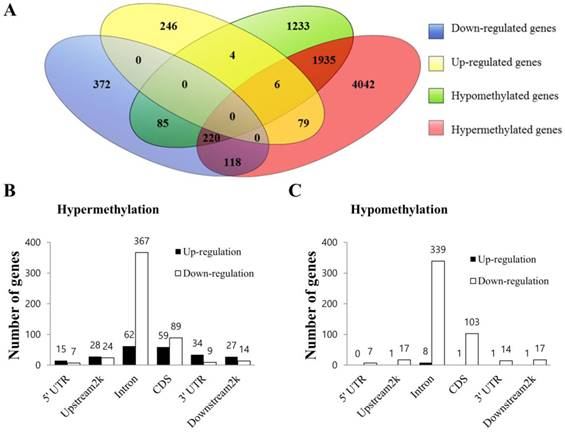
\includegraphics[width=0.8\textwidth]{journal-of-cancer_sample-result}}
	\caption{یک نمونه نمودار خلاصه برای نمایش نوآوری در نتایج
		%\cite{kim2016integrated}
	}
	\label{fig:sampleDiagram}
\end{figure}\\
طبیعتاً به صلاحدید نگارنده، شکل‌ها و نمودار‌ها می توانند در بخش های مختلف، خصوصا فصل
\ref{chap:results}
مورد استفاده قرار گیرند.

\subsection{تعریف واژه‌ها (اختیاری)}
در این قسمت محقق باید واژه‌هایی را که ممکن است برای خواننده آشنا نباشد، تعریف کند.

\subsection{خلاصه فصل‌ها}
در آخرین قسمتِ فصل اول پایان‌نامه، خلاصه‌ای اشاره‌وار از فصل‌های آتی آورده می‌شود تا خواننده بتواند تصویری واضح از دیگر قسمت‌های پایان‌نامه در ذهن خود ترسیم کند.

\section{جمع‌بندی}
در این فصل به دو مقولهٔ نحوه استفاده از قالب \پ دانشگاه تهران و نیز ویژگی‌هایی که محتویات فصل اول پایان‌نامه (یعنی مقدمه) باید داشته باشند، پرداخته شد. با توجه به اینکه این راهنما نحوه استفاده از قالب را شرح داده، ملزومات محتوایی هر فصل پایان‌نامه را توضیح می‌دهد و در پیوست‌ها نیز نحوهٔ کار با لاتک را یادآوری خواهد کرد، بنابراین مطالعهٔ کامل آن مقداری وقت شما را خواهد گرفت؛ اما مطمئن باشید از اتلاف وقت شما در ادامه کارتان تا حد زیادی جلوگیری خواهد کرد. در نوشتن متن حاضر سعی شده است علاوه بر ایجاد یک قالب لاتک برای پایان‌نامه‌های دانشگاه تهران، نکات محتوایی هر فصل نیز گوشزد گردد. طبیعتاً برای نگارش پایان‌نامهٔ خود می‌بایست مطالب تمام فصل‌ها را خودتان بازنویسی کنید.

در ادامهٔ این راهنما، تنها فصل‌هایی که یک پایان‌نامه باید داشته باشد و نیز خصوصیات یا ساختاری که محتویات هر فصل باید از آنها برخوردار باشد%
\footnote{از روی فایل «تمپلیت نگارش و تدوین پایان‌نامه \cite{UTThesisGuide}»}،
آورده می‌شوند. نهایتاً  در پیوست‌ها، مطالبی در باب یادآوری دستورات لاتک، نحوه نوشتن فرمول‌ها، تعاریف، قضایا، مثال‌ها، درج تصاویر، نمودارها، جداول و الگوریتم‌ها و نیز مدیریت مراجع، آمده است.

همچنین توصیه اکید دارم که رفع خطاهایی که احتمالاً با آنها مواجه می‌شوید را به آخر موکول نفرمایید و به محض برخورد با خطا، آن را اشکال‌زدایی و برطرف نمائید.!
و
\verb!% !TeX root=../main.tex
\chapter{مروری بر مطالعات انجام شده}
%\thispagestyle{empty} 
\section{مقدمه}
هدف از این فصل که با عنوان‌های  «مروری بر ادبیات موضوع%
\LTRfootnote{Literature Review}»،
«مروری بر منابع» و یا «مروری بر پیشینه تحقیق%
\LTRfootnote{Background Research}»
معرفی می‌شود، بررسی و طبقه‌بندی یافته‌های تحقیقات دیگر محققان در سطح دنیا و تعیین و شناسایی خلأهای تحقیقاتی است. آنچه را که تحقیق شما به دانش موجود اضافه می‌کند، مشخص کنید. طرح پیشینه تحقیق%
\LTRfootnote{Background Information}
یک مرور محققانه است و تا آنجا باید پیش برود که پیش‌زمینهٔ تاریخی مناسبی از تحقیق را بیان کند و جایگاه تحقیق فعلی را در میان آثار پیشین نشان دهد. برای این منظور منابع مرتبط با تحقیق را بررسی کنید، البته نه آنچنان گسترده که کل پیشینه تاریخی بحث را در برگیرد. برای نوشتن این بخش:
\begin{itemize}
	\item
	دانستنی‌های موجود و پیش‌زمینهٔ تاریخی و وضعیت کنونی موضوع را چنان بیان کنید که خواننده بدون مراجعه به منابع پیشین، نتایج حاصل از مطالعات قبلی را درک و ارزیابی کند.
	\item
	نشان دهید که بر موضوع احاطه دارید. پرسش تحقیق را همراه بحث و جدل‌ها و مسائل مطرح شده بیان کنید و مهم‌ترین تحقیق‌های انجام شده در این زمینه را معرفی نمائید.
	\item
	ابتدا مطالب عمومی‌تر و سپس پژوهش‌های مشابه با کار خود را معرفی کرده و نشان دهید که تحقیق شما از چه جنبه‌ای با کار دیگران تشابه یا تفاوت دارد.
	\item
	اگر کارهای قبلی را خلاصه کرده‌اید، از پرداختن به جزئیات غیرضروری بپرهیزید. در عوض، بر یافته‌ها و مسائل روش‌شناختی مرتبط و نتایج اصلی تأکید کنید و اگر بررسی‌ها و منابع مروری عمومی دربارهٔ موضوع موجود است، خواننده را به آنها ارجاع دهید.
\end{itemize}

\section{تعاریف، اصول و مبانی نظری}
این قسمت ارائهٔ خلاصه‌ای از دانش کلاسیک موضوع است. این بخش الزامی نیست و بستگی به نظر استاد راهنما دارد.

\section{مروری بر ادبیات موضوع}
در این قسمت باید به کارهای مشابه دیگران در گذشته اشاره کرد و وزن بیشتر این قسمت بهتر است به مقالات ژورنالی سال‌های اخیر (۲ تا ۳ سال) تخصیص داده شود. به نتایج کارهای دیگران با ذکر دقیق مراجع باید اشاره شده و جایگاه و تفاوت تحقیق شما نیز با کارهای دیگران مشخص شود. استفاده از مقالات ژورنال‌های معتبر در دو یا سه سال اخیر، می‌تواند به اعتبار کار شما بیافزاید.

\section{نتیجه‌گیری}
‌در نتیجه‌گیری آخر این فصل، با توجه به بررسی انجام شده بر روی مراجع تحقیق، بخش‌های قابل گسترش و تحقیق در آن حیطه و چشم‌اندازهای تحقیق مورد بررسی قرار می‌گیرند.	در برخی از تحقیقات، نتیجه نهایی فصل روش تحقیق، ارائهٔ یک چارچوب کار تحقیقی 
\lr{(research framework)}
است.!
را در فایل 
\lr{main.tex}،
غیرفعال%
\footnote{
برای غیرفعال کردن یک دستور، کافی است در ابتدای آن، علامت درصد انگلیسی (\%) بگذارید.
}
 کنید. در غیر این صورت، ابتدا مطالب دو فصل اول پردازش شده و سپس مطالب فصل ۳ پردازش می‌شود که این کار باعث طولانی شدن زمان پردازش می‌گردد. هر زمان که خروجی کل \پ را خواستید، تمام فصل‌ها را دوباره در
\lr{main.tex}
فعال نمائید.
بدیهتاً لازم نیست فصل‌های \پ را به ترتیب تایپ کنید. مثلاً می‌توانید ابتدا مطالب فصل ۳ را تایپ نموده و سپس مطالب فصل ۱ را تایپ کنید. 
\subsubsection{مراجع}
برای وارد کردن مراجع \پ کافی است فایل 
\lr{MyReferences.bib}
را باز کرده و مراجع خود را به شکل اقلام نمونهٔ داخل آن، وارد کنید.  سپس از \lr{bibtex} برای تولید مراجع با قالب مناسب استفاده نمائید. برای توضیحات بیشتر بخش \ref{Sec:Ref} از پیوست \ref{app:latexIntro} و نیز پیوست \ref{app:refMan} را ببینید.

\subsubsection{واژه‌نامه فارسی به انگلیسی و برعکس}
برای وارد کردن معادل فارسی اصطلاحات لاتین در متن و تهیه فهرست واژه‌نامه از آنها، از بستهٔ
\lr{glossaries}
و نرم‌افزار
\lr{xindy}
استفاده می‌شود. بدین منظور کافی است اصطلاحات لاتین و ترجمهٔ آنها را در فایل
\lr{words.tex}
وارد کرده و هر جای متن که خواستید با دستورات
\verb|gls{label}|
یا \verb|glspl{label}|
معادل فارسی مفرد یا جمع یک اصطلاح را بیاورید.

مثلا در اینجا، واژهٔ
«\gls{Action}»
برای بار اول و دوباره
«\gls{Action}»
برای بار دوم در متن ظاهر شده است.
جهت توضیحات بیشتر به پیوست
\ref{app:refMan}
مراجعه کنید.
\subsubsection{نمایه}
برای وارد کردن نمایه، باید از 
\lr{xindy}
استفاده کنید. 
%زیرا 
%\lr{MakeIndex}
%با حروف «گ»، «چ»، «پ»، «ژ» و «ک» مشکل دارد و ترتیب الفبایی این حروف را رعایت نمی‌کند. همچنین، فاصله بین هر گروه از کلمات در 
%\lr{MakeIndex}،
%به درستی رعایت نمی‌شود که باعث زشت شدن حروف‌چینی این قسمت می‌شود. 
راهنمای چگونگی کار با 
\lr{xindy} 
را می‌توانید در ویکی پارسی‌لاتک و یا مثالهای موجود در دی‌وی‌دی «مجموعه پارسی‌لاتک»، پیدا کنید.

\subsection{اگر سوالی داشتم، از کی بپرسم؟}
برای پرسیدن سوال‌های خود موقع حروف‌چینی با زی‌پرشین، می‌توانید به
\href{http://qa.parsilatex.com}{سایت پرسش و پاسخ پارسی‌لاتک}%
\LTRfootnote{http://qa.parsilatex.com}
یا
\href{http://forum.parsilatex.com}{بایگانی تالارگفتگوی قدیمی پارسی‌لاتک}%
\LTRfootnote{http://forum.parsilatex.com}
مراجعه کنید. شما هم می‌توانید روزی به سوال‌های دیگران در اینترنت جواب دهید.
بستهٔ زی‌پرشین و بسیاری از بسته‌های مرتبط با آن مانند
\lr{bidi} و
\lr{Persian-bib}،
مجموعه پارسی‌لاتک، مثالهای مختلف موجود در آن، قالب پایان‌نامه دانشگاههای مختلف و سایت پارسی‌لاتک همه به صورت داوطلبانه توسط افراد گروه پارسی‌لاتک و گروه
\lr{Persian TeX}
و بدون هیچ کمک مالی انجام شده‌اند. کار اصلی نوشتن و توسعه زی‌پرشین توسط آقای وفا خلیقی انجام شده است که این کار بزرگ را به انجام رساندند.
اگر مایل به کمک به گروه پارسی‌لاتک هستید به سایت این گروه مراجعه فرمایید:
\begin{center}
	\url{http://www.parsilatex.com}
\end{center}

\section{محتویات فصل اول یک پایان‌نامه}
فصل اول یک پایان‌نامه باید به مقدمه یا کلیات تحقیق بپردازد.
هدف از فصل مقدمه%
\LTRfootnote{Introduction}،
شرح مختصر مسأله تحقیق، اهمیت و انگیزه محقق از پرداختن به آن موضوع، بهمراه اشاره‌ای کوتاه به روش و مراحل تحقیق است. مقدمه، اولین فصل از ساختار اصلی \پ بوده و زمینه اطلاعاتی لازم را برای خواننده فراهم می‌آورد. در طول مقدمه باید سعی شود موضوع تحقیق با زبانی روشن، ساده و بطور عمیق و هدفمند به خواننده معرفی شود. این فصل باید خواننده را مجذوب و اهمیت موضوع تحقیق را آشکار سازد. در مقدمه باید با ارائهٔ سوابق، شواهد تحقیقی و اطلاعات موجود (با ذکر منبع) با روشی منظم، منطقی و هدف‌دار، خواننده را جهت داد و به سوی راه حل مورد نظر هدایت کرد. مقدمه مناسب‌ترین جا برای ارائهٔ اختصارات و بعضی توضیحات کلی است، توضیحاتی که شاید نتوان در مباحث دیگر آنها را شرح داد.

مقدمه، یکی از ارکان اساسی و اصلی پایان نامه است که مهمترین قسمت‌های آن عبارتند از: 

\subsection{عنوان تحقیق} 
باید شناختی دقیق و روشن از حوزهٔ موضوع تحقیق را عرضه دارد و خالی از هرگونه ابهام و پیچیدگی باشد.

\subsection{مسأله تحقیق}
وظیفه اصلی مقدمه بیان این مطلب به خواننده است که چرا انجام تحقیق را به عهده گرفته‌اید. اگر دلیل شما برای انجام این کار پاسخگویی به سؤال مورد علاقه‌تان است، با مشکل زیادی روبه‌رو نخواهید بود. یکی از بهترین روش‌ها برای نوشتن مقدمهٔ یک پایان‌نامه، طرح پرسش یا پرسش‌هایی مهم و اساسی است که کار تحقیقاتی شما از آغاز تا پایان قصد پاسخ دادن به آن را دارد. گاهی می‌توانید ابتدا اهمیت موضوع را بیان و سپس پرسش خود را در آن موضوع مطرح کنید.

\subsection{تاریخچه‌ای از موضوع تحقیق}
به طور کلی تشریح روندهای تحقیقاتی در محدودهٔ مورد مطالعه، مستلزم ارجاع به کارهای دیگران است. بعضی از نویسندگان برای کارهای دیگران هیچ اعتباری قائل نمی‌شوند و در مقابل، بعضی دیگر از نویسندگان در توصیف کارهای دیگران، بسیار زیاده‌روی می‌کنند. اکثر مواقع، ارجاع به مقالات دو سال قبل از کارتان، بهتر از نوشتن سطرهای مرجع است. در این قسمت باید به طور مختصر به نظرات و تحقیقات مربوط به موضوع و یا مسائل و مشکلات حل نشده در این حوزه و همچنین توجه و علاقه جامعه به این موضوع، اشاره شود.

\subsection{تعریف موضوع تحقیق}
در این قسمت محقق، موضوع مورد علاقه و یا نیاز احساس شدهٔ خود را در حوزه تحقیق بیان می‌دارد و عوامل موجود در موقعیت را تعریف و تعیین می‌کند.

\subsection{هدف یا هدف‌های کلی و آرمانی تحقیق}
این قسمت باید با جملات مثبت و کلی طرح شود و از طولانی شدن مطالب پرهیز شود.

\subsection{روش انجام تحقیق}
در این قسمت، پژوهشگر روش کاری خود را بیان می‌دارد و شیوه‌های گوناگونی را که در گردآوری مطالب خود بکار برده، ذکر می‌کند. همچنین اگر روش آماری خاصی را در تهیه و تدوین اطلاعات به کار برده است، آن شیوه را نیز اینجا بیان می‌کند.

\subsection{نوآوری، اهمیت و ارزش تحقیق}
در این قسمت، در مورد نوآوری علمی و عملی تحقیق که محقق به آن دست خواهد یافت، بحث می‌شود. ممکن است لازم باشد تا برخی نمودارهای خلاصه در این بخش استفاده شوند. به عنوان مثال، نموداری از مقاله
\cite{kim2016integrated}
در شکل
\ref{fig:sampleDiagram}
آمده است.
\begin{figure}[ht]
	\centerline{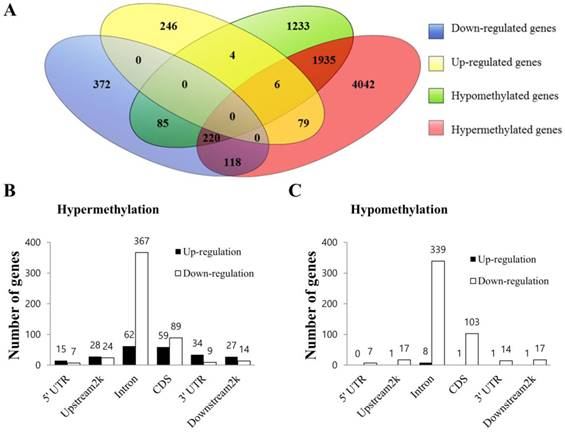
\includegraphics[width=0.8\textwidth]{journal-of-cancer_sample-result}}
	\caption{یک نمونه نمودار خلاصه برای نمایش نوآوری در نتایج
		%\cite{kim2016integrated}
	}
	\label{fig:sampleDiagram}
\end{figure}\\
طبیعتاً به صلاحدید نگارنده، شکل‌ها و نمودار‌ها می توانند در بخش های مختلف، خصوصا فصل
\ref{chap:results}
مورد استفاده قرار گیرند.

\subsection{تعریف واژه‌ها (اختیاری)}
در این قسمت محقق باید واژه‌هایی را که ممکن است برای خواننده آشنا نباشد، تعریف کند.

\subsection{خلاصه فصل‌ها}
در آخرین قسمتِ فصل اول پایان‌نامه، خلاصه‌ای اشاره‌وار از فصل‌های آتی آورده می‌شود تا خواننده بتواند تصویری واضح از دیگر قسمت‌های پایان‌نامه در ذهن خود ترسیم کند.

\section{جمع‌بندی}
در این فصل به دو مقولهٔ نحوه استفاده از قالب \پ دانشگاه تهران و نیز ویژگی‌هایی که محتویات فصل اول پایان‌نامه (یعنی مقدمه) باید داشته باشند، پرداخته شد. با توجه به اینکه این راهنما نحوه استفاده از قالب را شرح داده، ملزومات محتوایی هر فصل پایان‌نامه را توضیح می‌دهد و در پیوست‌ها نیز نحوهٔ کار با لاتک را یادآوری خواهد کرد، بنابراین مطالعهٔ کامل آن مقداری وقت شما را خواهد گرفت؛ اما مطمئن باشید از اتلاف وقت شما در ادامه کارتان تا حد زیادی جلوگیری خواهد کرد. در نوشتن متن حاضر سعی شده است علاوه بر ایجاد یک قالب لاتک برای پایان‌نامه‌های دانشگاه تهران، نکات محتوایی هر فصل نیز گوشزد گردد. طبیعتاً برای نگارش پایان‌نامهٔ خود می‌بایست مطالب تمام فصل‌ها را خودتان بازنویسی کنید.

در ادامهٔ این راهنما، تنها فصل‌هایی که یک پایان‌نامه باید داشته باشد و نیز خصوصیات یا ساختاری که محتویات هر فصل باید از آنها برخوردار باشد%
\footnote{از روی فایل «تمپلیت نگارش و تدوین پایان‌نامه \cite{UTThesisGuide}»}،
آورده می‌شوند. نهایتاً  در پیوست‌ها، مطالبی در باب یادآوری دستورات لاتک، نحوه نوشتن فرمول‌ها، تعاریف، قضایا، مثال‌ها، درج تصاویر، نمودارها، جداول و الگوریتم‌ها و نیز مدیریت مراجع، آمده است.

همچنین توصیه اکید دارم که رفع خطاهایی که احتمالاً با آنها مواجه می‌شوید را به آخر موکول نفرمایید و به محض برخورد با خطا، آن را اشکال‌زدایی و برطرف نمائید.!
و
\verb!% !TeX root=../main.tex
\chapter{مروری بر مطالعات انجام شده}
%\thispagestyle{empty} 
\section{مقدمه}
هدف از این فصل که با عنوان‌های  «مروری بر ادبیات موضوع%
\LTRfootnote{Literature Review}»،
«مروری بر منابع» و یا «مروری بر پیشینه تحقیق%
\LTRfootnote{Background Research}»
معرفی می‌شود، بررسی و طبقه‌بندی یافته‌های تحقیقات دیگر محققان در سطح دنیا و تعیین و شناسایی خلأهای تحقیقاتی است. آنچه را که تحقیق شما به دانش موجود اضافه می‌کند، مشخص کنید. طرح پیشینه تحقیق%
\LTRfootnote{Background Information}
یک مرور محققانه است و تا آنجا باید پیش برود که پیش‌زمینهٔ تاریخی مناسبی از تحقیق را بیان کند و جایگاه تحقیق فعلی را در میان آثار پیشین نشان دهد. برای این منظور منابع مرتبط با تحقیق را بررسی کنید، البته نه آنچنان گسترده که کل پیشینه تاریخی بحث را در برگیرد. برای نوشتن این بخش:
\begin{itemize}
	\item
	دانستنی‌های موجود و پیش‌زمینهٔ تاریخی و وضعیت کنونی موضوع را چنان بیان کنید که خواننده بدون مراجعه به منابع پیشین، نتایج حاصل از مطالعات قبلی را درک و ارزیابی کند.
	\item
	نشان دهید که بر موضوع احاطه دارید. پرسش تحقیق را همراه بحث و جدل‌ها و مسائل مطرح شده بیان کنید و مهم‌ترین تحقیق‌های انجام شده در این زمینه را معرفی نمائید.
	\item
	ابتدا مطالب عمومی‌تر و سپس پژوهش‌های مشابه با کار خود را معرفی کرده و نشان دهید که تحقیق شما از چه جنبه‌ای با کار دیگران تشابه یا تفاوت دارد.
	\item
	اگر کارهای قبلی را خلاصه کرده‌اید، از پرداختن به جزئیات غیرضروری بپرهیزید. در عوض، بر یافته‌ها و مسائل روش‌شناختی مرتبط و نتایج اصلی تأکید کنید و اگر بررسی‌ها و منابع مروری عمومی دربارهٔ موضوع موجود است، خواننده را به آنها ارجاع دهید.
\end{itemize}

\section{تعاریف، اصول و مبانی نظری}
این قسمت ارائهٔ خلاصه‌ای از دانش کلاسیک موضوع است. این بخش الزامی نیست و بستگی به نظر استاد راهنما دارد.

\section{مروری بر ادبیات موضوع}
در این قسمت باید به کارهای مشابه دیگران در گذشته اشاره کرد و وزن بیشتر این قسمت بهتر است به مقالات ژورنالی سال‌های اخیر (۲ تا ۳ سال) تخصیص داده شود. به نتایج کارهای دیگران با ذکر دقیق مراجع باید اشاره شده و جایگاه و تفاوت تحقیق شما نیز با کارهای دیگران مشخص شود. استفاده از مقالات ژورنال‌های معتبر در دو یا سه سال اخیر، می‌تواند به اعتبار کار شما بیافزاید.

\section{نتیجه‌گیری}
‌در نتیجه‌گیری آخر این فصل، با توجه به بررسی انجام شده بر روی مراجع تحقیق، بخش‌های قابل گسترش و تحقیق در آن حیطه و چشم‌اندازهای تحقیق مورد بررسی قرار می‌گیرند.	در برخی از تحقیقات، نتیجه نهایی فصل روش تحقیق، ارائهٔ یک چارچوب کار تحقیقی 
\lr{(research framework)}
است.!
را در فایل 
\lr{main.tex}،
غیرفعال%
\footnote{
برای غیرفعال کردن یک دستور، کافی است در ابتدای آن، علامت درصد انگلیسی (\%) بگذارید.
}
 کنید. در غیر این صورت، ابتدا مطالب دو فصل اول پردازش شده و سپس مطالب فصل ۳ پردازش می‌شود که این کار باعث طولانی شدن زمان پردازش می‌گردد. هر زمان که خروجی کل \پ را خواستید، تمام فصل‌ها را دوباره در
\lr{main.tex}
فعال نمائید.
بدیهتاً لازم نیست فصل‌های \پ را به ترتیب تایپ کنید. مثلاً می‌توانید ابتدا مطالب فصل ۳ را تایپ نموده و سپس مطالب فصل ۱ را تایپ کنید. 
\subsubsection{مراجع}
برای وارد کردن مراجع \پ کافی است فایل 
\lr{MyReferences.bib}
را باز کرده و مراجع خود را به شکل اقلام نمونهٔ داخل آن، وارد کنید.  سپس از \lr{bibtex} برای تولید مراجع با قالب مناسب استفاده نمائید. برای توضیحات بیشتر بخش \ref{Sec:Ref} از پیوست \ref{app:latexIntro} و نیز پیوست \ref{app:refMan} را ببینید.

\subsubsection{واژه‌نامه فارسی به انگلیسی و برعکس}
برای وارد کردن معادل فارسی اصطلاحات لاتین در متن و تهیه فهرست واژه‌نامه از آنها، از بستهٔ
\lr{glossaries}
و نرم‌افزار
\lr{xindy}
استفاده می‌شود. بدین منظور کافی است اصطلاحات لاتین و ترجمهٔ آنها را در فایل
\lr{words.tex}
وارد کرده و هر جای متن که خواستید با دستورات
\verb|gls{label}|
یا \verb|glspl{label}|
معادل فارسی مفرد یا جمع یک اصطلاح را بیاورید.

مثلا در اینجا، واژهٔ
«\gls{Action}»
برای بار اول و دوباره
«\gls{Action}»
برای بار دوم در متن ظاهر شده است.
جهت توضیحات بیشتر به پیوست
\ref{app:refMan}
مراجعه کنید.
\subsubsection{نمایه}
برای وارد کردن نمایه، باید از 
\lr{xindy}
استفاده کنید. 
%زیرا 
%\lr{MakeIndex}
%با حروف «گ»، «چ»، «پ»، «ژ» و «ک» مشکل دارد و ترتیب الفبایی این حروف را رعایت نمی‌کند. همچنین، فاصله بین هر گروه از کلمات در 
%\lr{MakeIndex}،
%به درستی رعایت نمی‌شود که باعث زشت شدن حروف‌چینی این قسمت می‌شود. 
راهنمای چگونگی کار با 
\lr{xindy} 
را می‌توانید در ویکی پارسی‌لاتک و یا مثالهای موجود در دی‌وی‌دی «مجموعه پارسی‌لاتک»، پیدا کنید.

\subsection{اگر سوالی داشتم، از کی بپرسم؟}
برای پرسیدن سوال‌های خود موقع حروف‌چینی با زی‌پرشین، می‌توانید به
\href{http://qa.parsilatex.com}{سایت پرسش و پاسخ پارسی‌لاتک}%
\LTRfootnote{http://qa.parsilatex.com}
یا
\href{http://forum.parsilatex.com}{بایگانی تالارگفتگوی قدیمی پارسی‌لاتک}%
\LTRfootnote{http://forum.parsilatex.com}
مراجعه کنید. شما هم می‌توانید روزی به سوال‌های دیگران در اینترنت جواب دهید.
بستهٔ زی‌پرشین و بسیاری از بسته‌های مرتبط با آن مانند
\lr{bidi} و
\lr{Persian-bib}،
مجموعه پارسی‌لاتک، مثالهای مختلف موجود در آن، قالب پایان‌نامه دانشگاههای مختلف و سایت پارسی‌لاتک همه به صورت داوطلبانه توسط افراد گروه پارسی‌لاتک و گروه
\lr{Persian TeX}
و بدون هیچ کمک مالی انجام شده‌اند. کار اصلی نوشتن و توسعه زی‌پرشین توسط آقای وفا خلیقی انجام شده است که این کار بزرگ را به انجام رساندند.
اگر مایل به کمک به گروه پارسی‌لاتک هستید به سایت این گروه مراجعه فرمایید:
\begin{center}
	\url{http://www.parsilatex.com}
\end{center}

\section{محتویات فصل اول یک پایان‌نامه}
فصل اول یک پایان‌نامه باید به مقدمه یا کلیات تحقیق بپردازد.
هدف از فصل مقدمه%
\LTRfootnote{Introduction}،
شرح مختصر مسأله تحقیق، اهمیت و انگیزه محقق از پرداختن به آن موضوع، بهمراه اشاره‌ای کوتاه به روش و مراحل تحقیق است. مقدمه، اولین فصل از ساختار اصلی \پ بوده و زمینه اطلاعاتی لازم را برای خواننده فراهم می‌آورد. در طول مقدمه باید سعی شود موضوع تحقیق با زبانی روشن، ساده و بطور عمیق و هدفمند به خواننده معرفی شود. این فصل باید خواننده را مجذوب و اهمیت موضوع تحقیق را آشکار سازد. در مقدمه باید با ارائهٔ سوابق، شواهد تحقیقی و اطلاعات موجود (با ذکر منبع) با روشی منظم، منطقی و هدف‌دار، خواننده را جهت داد و به سوی راه حل مورد نظر هدایت کرد. مقدمه مناسب‌ترین جا برای ارائهٔ اختصارات و بعضی توضیحات کلی است، توضیحاتی که شاید نتوان در مباحث دیگر آنها را شرح داد.

مقدمه، یکی از ارکان اساسی و اصلی پایان نامه است که مهمترین قسمت‌های آن عبارتند از: 

\subsection{عنوان تحقیق} 
باید شناختی دقیق و روشن از حوزهٔ موضوع تحقیق را عرضه دارد و خالی از هرگونه ابهام و پیچیدگی باشد.

\subsection{مسأله تحقیق}
وظیفه اصلی مقدمه بیان این مطلب به خواننده است که چرا انجام تحقیق را به عهده گرفته‌اید. اگر دلیل شما برای انجام این کار پاسخگویی به سؤال مورد علاقه‌تان است، با مشکل زیادی روبه‌رو نخواهید بود. یکی از بهترین روش‌ها برای نوشتن مقدمهٔ یک پایان‌نامه، طرح پرسش یا پرسش‌هایی مهم و اساسی است که کار تحقیقاتی شما از آغاز تا پایان قصد پاسخ دادن به آن را دارد. گاهی می‌توانید ابتدا اهمیت موضوع را بیان و سپس پرسش خود را در آن موضوع مطرح کنید.

\subsection{تاریخچه‌ای از موضوع تحقیق}
به طور کلی تشریح روندهای تحقیقاتی در محدودهٔ مورد مطالعه، مستلزم ارجاع به کارهای دیگران است. بعضی از نویسندگان برای کارهای دیگران هیچ اعتباری قائل نمی‌شوند و در مقابل، بعضی دیگر از نویسندگان در توصیف کارهای دیگران، بسیار زیاده‌روی می‌کنند. اکثر مواقع، ارجاع به مقالات دو سال قبل از کارتان، بهتر از نوشتن سطرهای مرجع است. در این قسمت باید به طور مختصر به نظرات و تحقیقات مربوط به موضوع و یا مسائل و مشکلات حل نشده در این حوزه و همچنین توجه و علاقه جامعه به این موضوع، اشاره شود.

\subsection{تعریف موضوع تحقیق}
در این قسمت محقق، موضوع مورد علاقه و یا نیاز احساس شدهٔ خود را در حوزه تحقیق بیان می‌دارد و عوامل موجود در موقعیت را تعریف و تعیین می‌کند.

\subsection{هدف یا هدف‌های کلی و آرمانی تحقیق}
این قسمت باید با جملات مثبت و کلی طرح شود و از طولانی شدن مطالب پرهیز شود.

\subsection{روش انجام تحقیق}
در این قسمت، پژوهشگر روش کاری خود را بیان می‌دارد و شیوه‌های گوناگونی را که در گردآوری مطالب خود بکار برده، ذکر می‌کند. همچنین اگر روش آماری خاصی را در تهیه و تدوین اطلاعات به کار برده است، آن شیوه را نیز اینجا بیان می‌کند.

\subsection{نوآوری، اهمیت و ارزش تحقیق}
در این قسمت، در مورد نوآوری علمی و عملی تحقیق که محقق به آن دست خواهد یافت، بحث می‌شود. ممکن است لازم باشد تا برخی نمودارهای خلاصه در این بخش استفاده شوند. به عنوان مثال، نموداری از مقاله
\cite{kim2016integrated}
در شکل
\ref{fig:sampleDiagram}
آمده است.
\begin{figure}[ht]
	\centerline{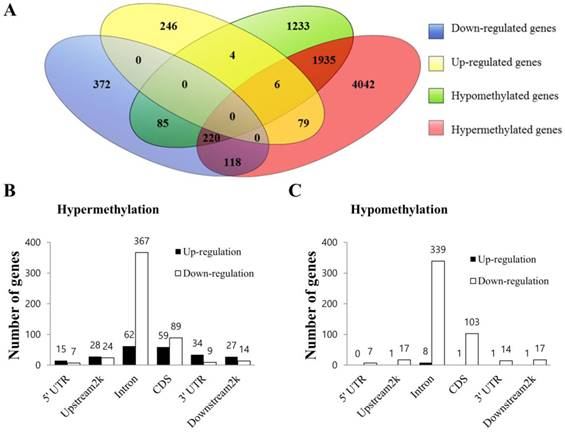
\includegraphics[width=0.8\textwidth]{journal-of-cancer_sample-result}}
	\caption{یک نمونه نمودار خلاصه برای نمایش نوآوری در نتایج
		%\cite{kim2016integrated}
	}
	\label{fig:sampleDiagram}
\end{figure}\\
طبیعتاً به صلاحدید نگارنده، شکل‌ها و نمودار‌ها می توانند در بخش های مختلف، خصوصا فصل
\ref{chap:results}
مورد استفاده قرار گیرند.

\subsection{تعریف واژه‌ها (اختیاری)}
در این قسمت محقق باید واژه‌هایی را که ممکن است برای خواننده آشنا نباشد، تعریف کند.

\subsection{خلاصه فصل‌ها}
در آخرین قسمتِ فصل اول پایان‌نامه، خلاصه‌ای اشاره‌وار از فصل‌های آتی آورده می‌شود تا خواننده بتواند تصویری واضح از دیگر قسمت‌های پایان‌نامه در ذهن خود ترسیم کند.

\section{جمع‌بندی}
در این فصل به دو مقولهٔ نحوه استفاده از قالب \پ دانشگاه تهران و نیز ویژگی‌هایی که محتویات فصل اول پایان‌نامه (یعنی مقدمه) باید داشته باشند، پرداخته شد. با توجه به اینکه این راهنما نحوه استفاده از قالب را شرح داده، ملزومات محتوایی هر فصل پایان‌نامه را توضیح می‌دهد و در پیوست‌ها نیز نحوهٔ کار با لاتک را یادآوری خواهد کرد، بنابراین مطالعهٔ کامل آن مقداری وقت شما را خواهد گرفت؛ اما مطمئن باشید از اتلاف وقت شما در ادامه کارتان تا حد زیادی جلوگیری خواهد کرد. در نوشتن متن حاضر سعی شده است علاوه بر ایجاد یک قالب لاتک برای پایان‌نامه‌های دانشگاه تهران، نکات محتوایی هر فصل نیز گوشزد گردد. طبیعتاً برای نگارش پایان‌نامهٔ خود می‌بایست مطالب تمام فصل‌ها را خودتان بازنویسی کنید.

در ادامهٔ این راهنما، تنها فصل‌هایی که یک پایان‌نامه باید داشته باشد و نیز خصوصیات یا ساختاری که محتویات هر فصل باید از آنها برخوردار باشد%
\footnote{از روی فایل «تمپلیت نگارش و تدوین پایان‌نامه \cite{UTThesisGuide}»}،
آورده می‌شوند. نهایتاً  در پیوست‌ها، مطالبی در باب یادآوری دستورات لاتک، نحوه نوشتن فرمول‌ها، تعاریف، قضایا، مثال‌ها، درج تصاویر، نمودارها، جداول و الگوریتم‌ها و نیز مدیریت مراجع، آمده است.

همچنین توصیه اکید دارم که رفع خطاهایی که احتمالاً با آنها مواجه می‌شوید را به آخر موکول نفرمایید و به محض برخورد با خطا، آن را اشکال‌زدایی و برطرف نمائید.	
% !TeX root=../main.tex
\chapter{دانش پیش‌زمینه}
%\thispagestyle{empty} 
\section{مقدمه}
در این فصل مفاهیم مورد نیاز و استفاده در این پروژه مورد بررسی قرار می‌گیرند.
این فصل، محل شرح کامل روش تحقیق است و بسته به نوع روش تحقیق و با نظر استاد راهنما می‌تواند «مواد و روش‌ها%
\LTRfootnote{Materials and Methods}»
نیز نام بگیرد. این فصل حدود ۱۵ صفحه است.

% \section{شبکه‌های مبتنی بر نرم‌افزار}

% \section{NetKAT}
نت‌کت، یک زبان برای توصیف شبکه‌های مبتنی بر نرم‌افزار است
\cite{netkat}.
این زبان با وجود سینتکس ساده‌ای که دارد، بر اساس
KAT
\cite{kat}
بنا شده و به همین دلیل یک سیستم معادلاتی کامل و صحیح دارد.
این سیستم معادلاتی کمک می‌کند تا با استفاده از روش‌های جبری و اثبات تساوی برنامه‌های توصیف شده در این زبان، در مورد آن‌ها استدلال کرد.

\subsection{سینتکس NetKAT}
در نت‌کت هر بسته به عنوان یک نگاشت از یک مجموعه از فیلد‌های
$f_1,f_2,...,f_n$
به اعداد طبیعی با تعداد ارقام ثابت در نظر گرفته می‌شود.
آی‌پی‌های مبدا و مقصد، نوع بسته، پورت‌های مبدا و مقصد مثال‌هایی از این فیلد‌ها هستند.
برای اینکه امکان استدلال در مورد مسیر‌های طی شده توسط یک بسته‌ در شبکه وجود داشته باشد،از مفهومی به نام تاریخچه‌ی بسته استفاده می‌شود.
هر تاریخچه‌ی بسته‌، یک دنباله از بسته‌ها است که بسته نخست دنباله، به عنوان بسته‌ی فعلی در نظر گرفته می‌شود.
سینتکس نت‌کت به صورت زیر تعریف می‌شود:
\begin{align*}
    a,b ::= & 1 | 0 | f = n | a + b | a \cdot b | \neg a  \\
    p,q ::= & a | f \la n | p + q | p \cdot q | p^* | dup
\end{align*}
به صورت شهودی
عبارت های ۱ و ۰ به ترتیب به معنای عبور دادن و رها کردن بدون شرط بسته هستند.
عبارت
$f=n$
در صورتی بسته را عبور می‌دهد که مقدار فیلد
f
آن برابر با
n
باشد.
عبارت
$f \la n$
مقدار n
را به فیلد f
بسته اختصاص می‌دهد.
به صورت دقیق، معنای هر عبارت با استفاده از معادلات زیر تعریف می‌شود:
\begin{align*}
    \sem{p}             & H \in \mathcal{P}({H})                \\
    \sem{1} h           & \teq \s{h}                            \\
    \sem{0} h           & \teq \s{}                             \\
    \sem{f=n}(pk::h)    & \teq \begin{cases}
                                   \s{pk::h} & \text{ if } pk.f = n \\
                                   \s{}      & \text{ otherwise }
                               \end{cases} \\
    \sem{\neq a}        & \teq \s{h} \setminus (\s{a}h)         \\
    \s{f \la n} (pk::h) & \teq \s{pk[f:=n]::h}                  \\
    \sem{p+q}h          & \teq \sem{p}h \cup \sem{q}h           \\
    \sem{p\cdot q} h    & \teq (\sem{p} \bullet \sem{q}) h      \\
    \sem{p^*}h          & \teq \bigcup_{i \in \mathbb{N}}F^i h  \\
    F^0 h               & \teq \s{h}                            \\
    F^{i+1} h           & \teq (\sem{p} \bullet F^i) h          \\
    (f \bullet g) x     & \teq \bigcup\s{g(y)|y \in f(x)}       \\
    \sem{dup} (pk::h)   & \teq \s{pk::(pk::h)}
\end{align*}
نت‌کت علاوه بر اصول موضوعه‌ی
KAT
اصول‌ موضوعه‌ی زیر را هم شامل می‌شود تا دستگاه معادلاتی کامل داشته باشد:
\begin{align}
    f \la n \cdot f' \la n' & \equiv f' \la n' \cdot f \la n,
    \text{ if } f \neq f' \label{mod-mod-comm}
    \\
    f \la n \cdot f' = n'   & \equiv f' = n' \cdot f \la n,
    \text{ if } f \neq f' \label{mod-filter-comm}                            \\
    dup \cdot f = n         & \equiv f = n \cdot dup \label{dup-filter-comm} \\
    f \la n \cdot f = n     & \equiv f \la n \label{mod-filter}              \\
    f = n \cdot f \la n     & \equiv f = n \label{filter-mod}                \\
    f \la n \cdot f \la n'  & \equiv f \la n' \label{mod-mod}                \\
    f = n \cdot f = n'      & \equiv 0, \text{ if } n \neq n' \label{contra} \\
    \Sigma_{i} f = i        & \equiv 1 \label{match-all}
\end{align}
اصل‌های
\ref{mod-mod-comm},\ref{mod-filter-comm},\ref{dup-filter-comm}
خواص جابه‌جایی عملیات‌ها را بیان می‌کنند.
اصل
\ref{mod-filter}
بیان می‌کند که اختصاص مقدار
n
به یک فیلد و سپس این فیلد با همین مقدار معادل با عملیات اختصاص به تنهایی است.
مشابه همین اصل برای یک فیلتر و سپس یک اختصاص هم در اصل
\ref{filter-mod}
مشخص شده.
اصل
\ref{mod-mod}
بیان می‌کند که در دنباله‌ای از اختصاص مقادیر به یک فیلد مشخص، تنها آخرین اختصاص تاثیر دارد.
در اصل
\ref{contra}
مشخص شده است که مقدار یک فیلد نمی‌تواند دو مقدار متفاوت داشته باشد.
در نهایت اصل
\ref{match-all}
بیان می‌کند که عملیات مجموع فیلتر‌ها به ازای هر مقدار ممکن برای یک فیلد مشخص برابر عنصر همانی است.
در ادامه نحوه‌ی پیاده‌سازی و درستی‌سنجی یک شبکه با استفاده از نت‌کت بیان می‌شود.
\begin{figure}
    \centering
    \begin{tikzpicture}[
            node distance={25mm},
            sw/.style = {draw, circle,minimum size=8mm},
            h/.style = {draw, rectangle,minimum size=8mm}
        ]
        \node[h] (h1)  {$H_1$};
        \node[sw] (sa) [right of=h1]  {$S_A$};
        \node[sw] (sb) [right of=sa] {$S_B$};
        \node[h] (h2)  [right of=sb] {$H_2$};
        \draw [thick] (h1)  -- node[above,pos=0.8]{1} (sa);
        \draw [thick] (sa) -- node[above,pos=0.2]{2}
        node[above,pos=0.8]{1}(sb);
        \draw [thick] (sb) -- node[above,pos=0.2]{2} (h2);
    \end{tikzpicture}
    \caption{مثال شبکه}
    \label{netkat:ssh}
\end{figure}
در شکل
\ref{netkat:ssh}
این شبکه شامل دو سوییچ
A و ‌B
و دو هاست می‌باشد.
هر سوییچ دو پورت دارد که با شماره‌های ۱ و۲ مشخص شده‌اند.
در این شبکه هدف این است که امکان جا‌به‌جایی همه‌ی بسته‌ها به غیر از بسته‌هایی که از نوع
SSH
هستند وجود داشته باشد.
عبارت نت‌کت زیر را در نظر بگیرید:
\begin{align*}
    p \triangleq (dst = H_1 \cdot pt \la 1) +
    (dst = H_2 \cdot pt \la 2)
\end{align*}
این عبارت همه‌ی بسته‌هایی که مقصد آن‌ها هاست ۱ باشد را به پورت ۱ و همه‌ی بسته‌هایی که مقصد‌ آن‌ها هاست ۲ باشد را به پورت شماره‌ی ۲ می‌فرستد.
این سیاست به سادگی رفتار سوییچ‌ها را در نت‌کت تعریف می‌کند.
در ادامه می‌توان با اضافه کردن یک فیلتر به این عبارت، دسترسی کنترل را به این سیاست اضافه کرد تا همه‌ی بسته‌های از نوع
SSH
رها شوند:
\begin{align*}
    p_{AC} \triangleq \neg(typ = SSH)\cdot p
\end{align*}
اما استفاده از عبارت بالا به تنهایی برای توصیف رفتار شبکه شکل
\ref{netkat:ssh}
کافی‌ نیست.
برای تکمیل این عبارت لازم است تا رفتار توپولوژی شبکه‌ هم به آن افزوده شود.
در نت‌کت توپولوژی شبکه به عنوان یک گراف جهت‌دار در نظر گرفته می‌شود و رفتار آن در قالب اجتماع رفتار هر یک از لینک‌های آن توصیف می‌شود.
برای شبکه‌ی شکل
\ref{netkat:ssh}
می‌توان از عبارت زیر برای توصیف توپولوژی شبکه استفاده کرد:
\begin{align*}
    t \triangleq & (sw = A \cdot pt = 2 \cdot sw \la B \cdot pt \la 1) +
                 & (sw = b \cdot pt = 1 \cdot sw \la A \cdot pt \la 2) +
                 & (sw = b \cdot pt = 2)
\end{align*}
در نت‌کت در صورتی که سیاست و توپولوژی شبکه در قالب عبارت‌هایی توصیف شده‌باشند،
رفتار کل شبکه در واقع دنباله‌ای از اعمال این عبارت‌ها به صورت یکی در میان است.
به عنوان مثال در شکل
\ref{netkat:ssh}
یک بسته از هاست ۱ ابتدا توسط سوییچ
A
پردازش شده، سپس روی لینک بین دو سوییچ جا به جا می‌شود و در نهایت توسط سوییچ
B
پردازش می‌شود.
در نت‌کت می‌توان این رفتار را به صورت
$p_{AC}\cdot t \cdot p_{AC}$
توصیف کرد.
با استفاده از همین شهود، رفتار کل شبکه را می‌توان در قالب عبارت زیر توصیف کرد:
\begin{align*}
    (p_{AC}\cdot t)^*
\end{align*}
در توصیف بالا فرض شده است که بسته‌ها می‌توانند به هر طریق ممکن وارد شبکه و از آن خارج شوند، اما این رفتار همیشه مورد قبول نیست.
به عنوان مثال در شبکه شکل
\ref{netkat:ssh}
می‌توانیم مکان‌های ورودی یا خروجی شبکه را در قالب عبارت زیر توصیف کنیم:
\begin{align*}
    p_{net} \triangleq e \cdot (p_{AC}\cdot t)^* e
\end{align*}
در حالت کلی‌تر، نیازی به توصیف ورودی و خروجی‌های شبکه در قالب یک عبارت نیست.
پس اگر فرض شود که مکان‌های ورودی شبکه توسط عبارت
$in$
و مکان‌های خروجی شبکه در قالب عبارت
$out$
توصیف شده‌ باشند، رفتار یک شبکه در نت‌کت به صورت زیر تعریف می‌شود:
\begin{align*}
    in \cdot (p\cdot t)^*\cdot out
\end{align*}
که عبارت
$p$
سیاست شبکه و عبارت
$t$
توپولوژی شبکه است.

درستی‌سنجی یک شبکه و بررسی خواص آن در نت‌کت با استفاده از بررسی تساوی عبارت یک شبکه با عبارت‌های دیگر انجام می‌شود.
به عنوان مثال در شبکه‌ی شکل
\ref{netkat:ssh}
برای بررسی اینکه همه‌ی بسته‌ها با نوع
SSH
از هاست ۱ رها می‌شوند کافی است تا تساوی زیر را بررسی کنیم:
\begin{equation}
    \begin{pmatrix}
          type = SSH \cdot sw = A \cdot pt = 1 \cdot \\
          (p_{AC}\cdot t) ^ * \cdot                  \\
          sw = B\cdot pt = 2
    \end{pmatrix}
    \equiv 0
\end{equation}
از طرفی برای بررسی یک خاصیت در شبکه، مثلا امکان فرستاده شدن‌ همه‌ی بسته‌هایی که از نوع
SSH
نیستند از هاست ۱ به هاست ۲
می‌توان به جای بررسی تساوی دو عبارت از نامساوی 
$p \leq q$
استفاده کرد. 
این نامساوی که خلاصه شده‌ی تساوی
$p + q \equiv q$
است بیان می‌کند که رفتار عبارت
$p$
بخشی از رفتار عبارت
$q$
است.
بنابراین برای بررسی این مساله که شبکه‌ی شکل
\ref{netkat:ssh}
به درستی کار می‌کند و فقط بسته‌های 
SSH
را رها می‌کند می‌توان نامساوی زیر را بررسی کرد:
\begin{equation}
    \begin{pmatrix}
          \neg(type = SSH) \cdot sw = A \cdot pt = 1 \cdot &\\
          sw \la B \cdot pt \la 2 &
    \end{pmatrix}
    \leq (p_{AC}\cdot t)^ *
\end{equation}

% \section{نت‌کت پویا}
نک‌کت‌ پویا
\lf{DyNetKAT}
برای رفع برخی از کاستی‌های نت‌کت ارائه شده است
\cite{dynetkat}.
به صورت دقیق‌تر نت‌کت پویا، امکان توصیف به‌روز‌رسانی سیاست‌های شبکه و همچنین رفتار شبکه در مقابل چندین بسته را ممکن می‌سازد.

\subsection{دستور زبان نت‌کت پویا}
در نت‌کت‌ پویا، از رفتار انتها به انتها‌ی توصیف‌های شبکه در قالب عبارت‌های نت‌کت استفاده می‌شود.
به همین منظور سینتکس نت‌کت‌ پویا به صورت زیر تعریف می‌شود:
\begin{align*}
    N & :: = \mathrm{NetKAT}^{-dup}                    \\
    D & :: = \bot | N;D | x?N;D | x!N;D | D\parallel D
    D \oplus D | X                                     \\
      & X \triangleq D
\end{align*}
در سینتکس بالا
$\mathrm{NetKAT}^{-dup}$
قسمتی از زبان نت‌کت است که عبارت‌های
$dup$
از آن حذف شده است.
عبارت‌های
$dup$
در توصیف‌های نت‌کت تاثیری در رفتار یک عبارت ندارند و هدف از استفاده از آن‌ها ثبت یک اثر از هر بسته پس از پردازش توسط یکی از عناصر شبکه است و امکان استدلال بر روی رفتار شبکه را ممکن می‌سازد.
با توجه به این که در نت‌کت پویا رفتار انتها به انتهای یک عبارت نت‌کت مورد استفاده است، عبارت
$dup$
از دستور زبان کنار گذاشته شده است.
نت‌کت‌پویا یک لیست از بسته‌های ورودی را پردازش می‌کند و یک لیست از مجموعه‌ی بسته‌های خروجی تولید می‌کند.
اپراتور ترکیب متوالی
\lf{Sequential Composition}
$N;D$
باعث می‌شود که یک بسته از لیست بسته‌های ورودی توسط سیاست
$N$
پردازش شود و سپس بسته‌ی توسط عبارت
$D$
پردازش می‌شود.
در نت‌کت پویا امکان ارتباط توسط عبارت‌هایی به شکل
$x!N$
و
$x?N$
توصیف می‌شوند که به ترتیب ارسال و دریافت یک عبارت نت‌کت را روی کانال
$x$
توصیف می‌کنند.
ترکیب موازی
\lf{Parallel Composition}
دو عبارت توسط
$D \parallel D$
توصیف می‌شود.
در نهایت رفتار‌های غیرقطعی
\lf{Non-Deterministic}
توسط‌ عبارت‌هایی به شکل
$D \oplus D$
توصیف می‌شوند.

\subsection{معنای عملیاتی نت‌کت پویا}
معنای عملیاتی
\lf{Operational Seamntic}
نت‌کت پویا با استفاده از عبارت‌هایی به شکل
$(d,H,H')$
تعریف می‌شوند که
$d$
عبارت نت‌کت‌ پویا فعلی است،
$H$
لیست بسته‌هایی که در ادامه باید پردازش شوند
و
$H'$
لیست بسته‌هایی است که به صورت موفقیت‌آمیز توسط شبکه پردازش شده‌اند.
در اینجا فرض می شود که
$F = \s{f_1,...,f_n}$
یک مجموعه از فیلد‌های بسته‌ها است.
یک بسته به شکل یک تابع
$F \ra \mathbb{N}$
توصیف می‌شود.
برای یک بسته مانند
$\sigma$
تساوی
$\sigma(f_i) = v_i$
بیان می‌کند که مقدار فیلد
$f_i$
در بسته‌ی
$\sigma$
برابر با
$v_i$
است.
یک لیست خالی از بسته‌ها با
$\his{}$
نمایش داده می‌شود.
اگر
$l$
یک لیست از بسته‌ها باشد
$e::l$
لیستی است که حاصل از اضافه کردن بسته
$\sigma$
به ابتدای لیست به دست می‌آید.
برچسب هر قانون که با
$\gamma$
مشخص می‌شود به صورت یکی از شکل‌های
$(\sigma,\sigma'),x!q,x?q$
یا
$rcfg(x,q)$
تعریف می‌شود
که
$rcfg(x,q)$
به معنی انجام شدن
$x!q$
و
$x?q$
به صورت همگام
\lf{Synchronized}
است.
قوانین زیر معنای عملیاتی نت‌کت پویا را تعریف می‌کنند:
\begin{align}
     & (cpol^{\checkmark}_{\_;})
    \frac{\sigma' \in \sem{p}(\sigma::\his{})}
    {(p;q,\sigma::H,H')\xrightarrow{(\sigma,\sigma')}
    (q,H,\sigma'::H') }    \label{os:term}                                 \\
     & (cpol_X)
    \frac{(p,H_0,H_1)\xrightarrow{\gamma}(p',H_0',H_1')}
    {(X,H_0,H_1)\xrightarrow{\gamma}(p',H_0',H_1')}
    X \triangleq p         \label{os:recr}                                 \\
     & (cpol_{\_\oplus})
    \frac{(p,H_0,H_0')\xrightarrow{\gamma}(p',H_1,H_1')}
    {(p\oplus q,H_0,H_0')\xrightarrow{\gamma}(p',H_1,H_1')}
    \label{os:orr}                                                         \\
     & (cpol_{\oplus\_})
    \frac{(q,H_0,H_0')\xrightarrow{\gamma}(q',H_1,H_1')}
    {(p\oplus q,H_0,H_0')\xrightarrow{\gamma}(p',H_1,H_1')} \label{os:orl} \\
     & (cpol_{\_\parallel})
    \frac{(p,H_0,H_0')\xrightarrow{\gamma}(p',H_1,H_1')}
    {(p\parallel q,H_0,H_0')\xrightarrow{\gamma}(p' \parallel q,H_1,H_1')}
    \label{os:parr}                                                        \\
     & (cpol_{\parallel\_})
    \frac{(q,H_0,H_0')\xrightarrow{\gamma}(q',H_1,H_1')}
    {(p\parallel q,H_0,H_0')\xrightarrow{\gamma}(p \parallel q',H_1,H_1')}
    \label{os:parl}                                                        \\
     & (cpol_?)
    \frac{}
    {(x?p;q,H,H')\xrightarrow{x?p}(q,H,H')}
    \label{os:recv}                                                        \\
     & (cpol_!)
    \frac{}
    {(x!p;q,H,H')\xrightarrow{x!p}(q,H,H')}
    \label{os:send}                                                        \\
     & (cpol_{!?})
    \frac{
        (q,H,H') \xrightarrow{x!p}(q',H,H')
        (s,H,H') \xrightarrow{x?p} (s',H,H')
    }{
        (q\parallel,H,H') \xrightarrow{rcfg(x,p)} (q'\parallel s',H,H')
    }     \label{os:syncr}                                                 \\
     & (cpol_{?!})
    \frac{
        (q,H,H') \xrightarrow{x?p}(q',H,H')
        (s,H,H') \xrightarrow{x!p} (s',H,H')
    }{
        (q\parallel,H,H') \xrightarrow{rcfg(x,p)} (q'\parallel s',H,H')
    } \label{os:syncl}
\end{align}
قانون 
\ref{os:term}
انجام یک عملیات مانند
$(\sigma,\sigma')$
که به معنای
پردازش بسته‌ی ابتدایی لیست ورودی توسط عبارت 
$p$
و افزودن خروجی حاصل از آن مانند 
$\sigma'$
به لیست خروجی است را مشخص می‌کند.
قانون 
\ref{os:recr}
بیان می‌کند که رفتار متغیر 
$X$
که برابر با عبارت 
$p$
است معادل با رفتار عبارت 
$p$
است.
قوانین 
\ref{os:orr}
و
\ref{os:orl}
رفتار غیرقطعی را توصیف می‌کنند.
قوانین
\ref{os:parr}
و
\ref{os:parl}
رفتار دو عبارت موازی را توصیف می‌کنند.
قوانین
\ref{os:recv}
و
\ref{os:send}
مشخص می‌کنند که ارسال یا دریافت پیام در نت‌کت پویا پردازشی روی بسته‌ها انجام نمی‌دهد.
در نهایت همگام‌سازی
\lf{Synchronization}
ارسال و دریافت پیام توسط قوانین 
\ref{os:recv}
و
\ref{os:send}
توصیف شده است.


\begin{figure}
    \centering
    \begin{tikzpicture}[
            node distance={25mm},
            sw/.style = {draw, circle,minimum size=8mm},
            h/.style = {draw, rectangle,minimum size=8mm}
        ]
        \node[h] (i)  {$I$};
        \node[sw] (s) [right of=i]  {$S$};
        \node[h] (e)  [right of=s] {$E$};
        \draw [thick] (i)  -- node[above,pos=0.8]{$int$} (s);
        \draw [thick] (s) -- node[above,pos=0.2]{$ext$} (e);
    \end{tikzpicture}
    \caption{مثال دیوار آتش}
    \label{dynetkat:firewall}
\end{figure}

در ادامه چگونگی توصیف مثال دیوار آتش در شکل
\ref{dynetkat:firewall}
بیان می‌شود.
در این شبکه هدف این است که امکان ارتباط از داخل شبکه فراهم باشد ولی امکان ارسال بسته از خارج شبکه ممکن نباشد.
اما زمانی که یک بسته به خارج ارصال شد، دیوار آتش اجازه‌ی عبور بسته‌ها از بیرون را می‌دهد تا پاسخ بسته‌ها داده شود.
برای توصیف این شبکه می‌توان از عبارت نت‌کت پویای زیر استفاده کرد:
\begin{align*}
    Host  \triangleq   & secConReq!1;Host \oplus secConEnd!1;Host        \\
    Switch \triangleq  & (port = int) \cdot (port \la ext);Switch \oplus \\
                       & (port = ext)\cdot 0 ; Switch \oplus             \\
                       & secConReq?1;Switch'                             \\
    Switch' \triangleq & (port =int) \cdot (port \la ext);Switch' \oplus \\
                       & (port=ext)\cdot(port\la int);Switch' \oplus     \\
                       & secConEnd?1;Switch                              \\
    Init \triangleq    & Host \parallel Switch
\end{align*}
در این توصیف هاست امکان ارسال پیام برای شروع یا خاتمه‌ی یک ارتباط امن را دارد.
رفتار سوییچ در ابتدا به این صورت تعریف شده است که بسته‌ها را از پورت داخلی به پورت خارجی ارسال کند و تمام بسته‌هایی که از پورت خروجی وارد می‌شوند رها کند.
همچنین سوییچ امکان دریافت پیام شروع ارتباط امن را دارد.
پس از دریافت این پیام سوییچ اجازه می‌دهد تا بسته‌ها از پورت خروجی وارد شبکه شوند.
همچنین در صورتی که پیام خاتمه‌ی ارتباط امن را دریافت کند دوباره به رفتار اولیه‌ی خود بر می‌گردد.
در نهایت رفتار کل شبکه با استفاده از ترکیب موازی یک هاست و یک سوییچ در حالت اولیه توصیف می‌شود.
\begin{figure}[ht]
    \centerline{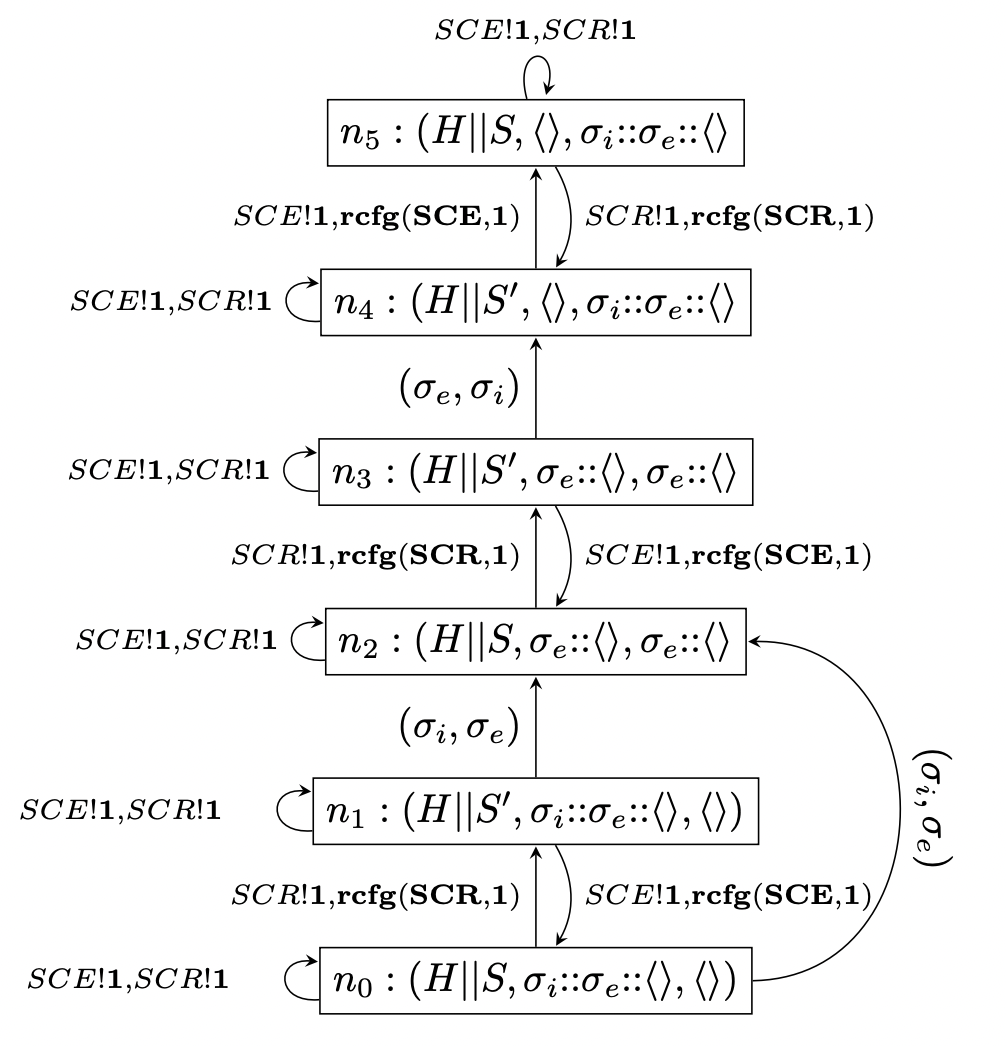
\includegraphics[width=0.8\textwidth]{mine/firewall-lts.png}}
    \caption{سیستم انتقال برچسب‌دار برای شبکه‌ی دیوار آتش}
    \label{firewall:lts}
\end{figure}
نمودار نمایش داده شده در شکل
\ref{firewall:lts}
سیستم انتقال این شبکه‌ را در حالتی که یک بسته روی پورت ورودی و یک بسته روی پورت خروجی شبکه وجود دارد نشان می‌دهد.
همانطور که در نمودار مشخص است، عملیات
$(\sigma_e,\sigma_i)$
که به معنای ارسال بسته از پورت ورودی به پورت خروجی است تنها در قسمتی از این سیستم انتقال قابل دسترسی است که پیش از آن یکی از عملیات‌های
$SCR?1$
یا
$rcfg(SCR,1)$
انجام شده باشند.
بنابراین در این حالت شبکه تنها در صورتی که بسته خارجی را به داخل ارسال می‌کند که پیش از آن پیام آغاز ارتباط امن دریافت کرده‌ باشد.



% \section{ساختمان رویداد}
ساختمان رویداد
\lf{Event Structure}
\cite{es}
یک مدل محاسباتی
\lf{Computational Model}
برای پردازه‌های هم‌روند
\lf{Concurrent}
است.
ساختمان رویداد یک مدل غیر جای‌گذاری
\lf{Non-Interleaving}
شده است.
در این مدل، برخلاف مدل‌های جایگذاری شده مانند سیستم‌انتقال که هم‌روندی پردازه‌های موازی با انتخاب غیرقطعی مدل می‌شود، هم‌روندی پردازه‌ها به صورت صریح در مدل توصیف می‌شوند.
\begin{definition}{ساختمان رویداد}
    یک ساختمان رویداد یک سه‌تایی
    $(E,\#,\vdash)$
    است که در آن:
    \begin{enumerate}
        \item $E$
              یک مجموعه از رویداد‌ها است
        \item $\#$
              رابطه‌ی تعارض
              \lf{Conflict}
              ، یک رابطه‌ی دودویی متقارن و غیربازتابی بر روی مجموعه‌ی
              $E$
              است
        \item $\vdash \subseteq Con \times E$
              رابطه‌ی فعال سازی
              \lf{Enabling}
              است که شرط زیر را برقرار می‌کند:
              \begin{align*}
                  X \vdash e \wedge X \subseteq Y \in Con
                  \Rightarrow Y \vdash e
              \end{align*}
    \end{enumerate}
    در رابطه‌ی بالا
    $Con$
    زیرمجموعه‌ای از مجموعه‌ی توانی رویدادها است که اعضای آن فاقد تعارض باشند.
    به صورت دقیق‌تر داریم:
    \begin{align*}
        Con = \s{X \subseteq E| \forall e,e' \in X. \neg(e\#e')}
    \end{align*}
\end{definition}
برای مشخص کردن وضعیت یک سیتم در هر لحظه از مفهومی به نام پیکر‌بندی
\lf{Configuration}
استفاده می‌شود و
و یک مجموعه شامل رویدادهایی است که تا آن لحظه در سیستم رخ داده‌اند.
\begin{definition}{پیکربندی}
    اگر
    $\mathrm{E} = (E,\#,\vdash)$
    یک ساختمان رویداد باشد، یک پیکربندی آن یک زیرمجموعه از رویداد‌ها
    $x \subseteq E$
    است که شرایط زیر را داشته باشد:
    \begin{enumerate}
        \item $x \in Con$
        \item $\forall e \in x \exists e_0,...,e_n \in x. e_n = e \ \&
                  \forall i \leq n. \s{e_0,...,e_{i-1}} \vdash e_i$
    \end{enumerate}
\end{definition}
مجموعه‌ی همه‌ی پیکربندی‌های یک ساختمان رویداد مانند
$\mathrm{E}$
با
$\mathcal{F}(\mathrm{E})$
نمایش داده می‌شود.

\begin{figure}
    \centering
    \begin{tikzpicture}[node distance={15mm},minimum size=10mm,
            main/.style = {draw, circle}]
        \node[main] (S)  {$s$};
        \node[main] (H1) [above of=S,left of=S] {$h_1$};
        \node[main] (H2) [above of=S,right of=S] {$h_2$};
        \draw[->,thick] (H1) -- (S);
        \draw[<-,thick] (S) -- (H2);
    \end{tikzpicture}
    \caption{}
    \label{fig:es:update}
\end{figure}
شبکه‌ی موجود در شکل
\ref{fig:es:update}
را در نظر بگیرید.
در این شبکه دو هاست ۱ و ۲ به صورت هم‌روند یک بسته را به سوییچ ارسال می‌کنند.
این بسته‌ها شامل اطلاعات برای به روزرسانی مسیر‌های دیگر در شبکه هستند، بنابراین سوییچ پس از دریافت هر دوی این بسته‌ها آن ها را پردازش کرده و مسیر‌های خود را به روزرسانی می‌کند.
برای مدل کردن این شبکه می‌توانیم از یک ساختمان رویداد به صورت زیر استفاده کنیم:
\begin{align*}
    \mathrm{E} & = (
    \s{r_1,r_2,u},
    \e, \s{(\e,r_1),(\e,r_2),(\s{r_1,r_2},u)}
    )
\end{align*}
در این ساختمان رویداد، رویداد‌ها به ترتیب دریافت یک بسته از هاست ۱، دریافت یک بسته از هاست ۲ و به روز رسانی سوییچ را مدل می‌کنند.
یکی از روش‌های رسم نمودار برای ساختمان رویداد، رسم نمودار هس
\lf{Hasse}
برای مجموعه‌ی پیکربندی‌های این ساختمان رویداد بر اساس رابطه‌ی زیرمجموعه است.
برای مثالی که بیان شد می‌توان نموداری مطابق شکل
\ref{fig:es:configs}
زیر را رسم کرد:
\begin{figure}
    \centering
    \begin{tikzpicture}[scale=0.8]
        \crd{0}{0}{$\emptyset$}
        \crd[left]{-2}{1}{$\s{r_1}$}
        \crd[right]{2}{1}{$\s{r_2}$}
        \crd[right]{0}{2}{$\s{r_1,r_2}$}
        \crd[right]{0}{3}{$\s{r_1,r_2,u}$}
        \draw [ultra thick] (0,0) -- (2,1);
        \draw [ultra thick] (0,0) -- (-2,1);
        \draw [ultra thick] (-2,1) -- (0,2);
        \draw [ultra thick] (2,1) -- (0,2);
        \draw [ultra thick] (0,2) -- (0,3);
    \end{tikzpicture}
    \caption{}
    \label{fig:es:configs}
\end{figure}


\section{مدل علی}
پیدا کردن تعریفی برای علت واقعی
\lf{Actual Cause}
مبحثی است که مورد مطالعه و تحقیق بسیاری قرار گرفته است.
این مساله به طور خاص در متون فلسفه مورد توجه قرار گرفته است.
یکی از تعاریف علت واقعی که مورد توجه بسیاری قراری گرفته است، تعریفی مبتنی بر وابستگی خلاف واقع
\lf{Counterfactual}
است.
مطابق این تعریف، رویداد الف علت رویداد ب است اگر در شرایطی که رویداد الف اتفاق نیافته باشد، رویداد ب هم اتفاق نیافتند.
در اینجا اتفاق نیفتادن رویداد الف خلاف واقع است، چون در سناریوی واقعی 
(سناریو ای که واقعا اتفاق افتاده و مشاهده شده است)
رویداد الف اتفاق افتاده است و در نظر گرفتن شرایطی که در آن رویداد الف اتفاق نیفتاده باشد بر خلاف واقعیت موجود است.
اما این مدل به تنهایی امکان پیدا کردن علت مناسب را در همه‌ی موارد ندارد.
به عنوان مثال سناریوی زیر را در نظر بگیرید که در آن سارا و بهرام هر کدام یک سنگ را برداشته و به سمت یک بطری شیشه‌ای پرتاب می‌کنند.
در این سناریو، سنگ سارا زودتر از سنگ بهرام به بطری برخورد کرده و در نتیجه آن را می‌شکند.
در این سناریو واضح است که پرتاب سنگ توسط سارا علت شکسته شدن بطری است.
فرض کنید بخواهیم از علیت مبتنی بر خلاف واقع برای پیدا کردن این علت استفاده کنیم.
بنابراین باید شرایطی را در نظر بگیریم که سارا سنگ خود را پرتاب نکند.
اما مشکل اینجاست که در این شرایط همچنان بطری شکسته می‌شود، چون اگر سارا سنگ خود را پرتاب نکند، بهرام همچنان سنگ خود را پرتاب می‌کند و در نتیجه این بار سنگ بهرام به بطری برخورد کرده و آن را می‌شکند.
بنابراین در این سناریو امکان تعریف پرتاب سنگ سارا به عنوان علت شکسته شدن بطری با استفاده از استدلال مبتنی بر خلاف واقع وجود ندارد.
هالپرن
\lf{Halpern}
 و پرل
 \lf{Pearl}
 برای حل کردن مشکلاتی از این دست، تعریف جدیدی از علت واقعی
\cite{hp}
ارائه کردند.
مدل ارائه شده توسط آن‌ها به دلیل اینکه بر پایه ریاضی بنا شده است امکان استفاده از آن را در آنالیز و تحلیل سیستم‌های محاسباتی فراهم می‌کند.
به همین دلیل این تعریف در مقالات زیادی در حوزه‌ی دانش کامپیوتر مورد استفاده قرار گرفته است.

برای تعریف علت واقعی ابتدا برخی مفاهیم اولیه مورد استفاده در این تعریف توضیح داده می‌شوند.

به صورت کلی فرض می‌شود که دنیای مورد تحلیل توسط تعدادی متغیر تصادفی مدل شده است.
اگر
$X$
یک متغیر تصادفی باشد، یک رویداد به شکل
$X=x$
تعریف می‌شود.
برخی از این متغیر‌ها بر روی یکدیگر تاثیر گذارند.
این وابستگی‌ها در قالب مجموعه‌ای از معادلات ساختاری
\lf{Structural Equations}
مدل می‌شوند.
هر یک از این معادلات در واقع یک مکانیزم یا قانون مشخص در این دنیا را مدل می‌کنند.
متغیرها به دو دسته درونی
\lf{Endogenous}
و برونی
\lf{Exogenous}
تقسیم می‌شوند.
متغیر‌های برونی متغیر‌هایی در نظر گرفته می‌شوند که مقدار آن‌ها توسط عواملی که درون مدل نیستند تعیین می‌شوند.
بنابراین در مدل فرض می‌شود که مقدار این متغیر‌ها از قبل مشخص است.
اما متغیر‌های درونی متغیرهایی هستند که مقدار آن‌ها بر اساس معادلات ساختاری تعیین می‌شود.
به صورت دقیق‌تر، امضای
\lf{Signature}
یک مدل یک سه‌تایی
$\mc{S} = (\mc{U},\mc{V},\mc{R})$
است که در آن
$\mc{U}$
مجموعه‌ی متغیر‌های بیرونی
$\mc{V}$
مجموعه‌ی متغیر‌های درونی و
$\mc{R}$
دامنه‌ی مقادیر ممکن برای هر یک از متغیر‌ها را مشخص می‌کند.
در این مدل فرض می‌شود که مجموعه‌ی متغیر‌های درونی محدود است.
مدل علی بر روی یک امضای
$\mc{S}$
یک دوتایی
$\mc{M} = (\mc{S},\mc{F})$
است که در آن
$\mc{F}$
به هر متغیر داخلی
$X \in \mc{V}$
یک تابع
$F_X: (\times_{U\in \mathcal{U}}\mathcal{R}(U))\times (\times_{Y\in\mathcal{V}-\{X\}}\mathcal{R}(Y))\rightarrow \mathcal{R}(X)$
اختصاص می‌دهد.
هر تابع، معادله‌ی یک متغیر را به ازای مقادیر تمام متغیر‌های دیگر مشخص می‌کند.
به عنوان مثال اگر فرض کنیم
$F_X(Y,Z,U) = Y + U$
اگر داشته باشیم
$Y=3, U=2$
آنگاه مقدار
$X$
برابر ۵ خواهد شد.
این معادلات امکان تفسیر آن‌ها بر اساس شرایط خلاف واقع را می‌دهند.
به عنوان مثال در همین مدل اگر فرض کنیم که
$U=u$
می‌توانیم نتیجه بگیریم که اگر مقدار متغیر
$Y$
برابر ۴ باشد آنگاه مستقل از اینکه مقدار بقیه‌ی متغیر‌ها در دنیای واقعی چه مقداری دارند، مقدار متغیر
$X$
برابر
$u+4$
خواهد بود که به صورت
$(M,u) \vDash [Y \la 4](X = u + 4)$
نوشته می‌شود.
توابع ذکر شده فقط برای متغیر‌های درونی تعریف می‌شوند و همانطور که پیش‌تر اشاره شد، برای متغیرهای بیرونی تابعی تعریف نمی‌شود و فرض می‌شود که مقدار آن‌ها از قبل مشخص شده است.

\begin{example}
    \label{ex:hp:fire}
    یک جنگل را در نظر بگیرید که می‌تواند توسط رعد و برق یا یک کبریت رها شده دچار آتش سوزی شود.
    برای مدل کردن این سناریو از سه متغیر بولی
    \lf{Boolean}
    استفاده می‌کنیم:
    \begin{itemize}
        \item متغیر
              $F$
              که اگر جنگل دچار آتش سوزی شود مقدار آن درست است و در غیر این صورت مقدار آن غلط است
        \item متغیر
              $L$
              که اگر رعد و برق اتفاق افتاده باشد مقدار آن درست است و در غیر این صورت غلط است
        \item متغیر
              $M$
              که اگر یک کبریت در جنگل رها شده باشد مقدار آن درست است و در غیر این صورت غلط است
    \end{itemize}
\end{example}
در این مثال فرض می کنیم که مقادیر متغیر‌های برونی به گونه‌ای است که تمام شرایط لازم برای آتش سوزی جنگل در صورتی که رعد و برق اتفاق بیافتد یا کبریتی در جنگل رها شود را دارد
(به عنوان مثال درختان جنگل به اندازه‌ی کافی خشک هستند و اکسیژن کافی در هوا وجود دارد).
در این مدل تابع متغیر
$F$
را به گونه‌ای تعریف می‌کنیم که داشته باشیم:
$F_F(\vec u, L , M) = L \vee M$.
همانطور که پیش‌تر بیان شد، این مدل علی امکان بررسی معادلات بر اساس شرایط خلاف واقع را می‌دهد.
به صورت دقیق‌تر اگر
$M = (\mc{S},\mc{F})$
یک مدل علی،
$\vec X$
یک بردار از متغیرهای درونی و
$\vec{x}, \vec{u}$
برداری از مقادیر متغیر‌های
$\vec{X},\mc{U}$
باشند
مدل
$M_{\vec{X}\la \vec{x}}$
را با امضای
$S_{\vec X}=(\mc{U},\mc{V}-\vec X,\mc{R}|_{\mc - \vec{X}})$
یک زیرمدل
\lf{Sub-Model}
از
$M$
تعریف می‌کنیم.
به صورت شهودی این مدل حاصل مداخله‌
\lf{Intervention}
ای در مدل
$M$
است که در آن مقادیر
$\vec{x}$
را به متغیر‌های
$\vec{X}$
اختصاص داده‌ایم.
به صورت دقیق‌تر تعریف می‌کنیم
$M_{\vec{X}\la\vec{x}} = (\mc{S}_{\vec{X}},\mc{F}^{\vec{X}\la\vec{x}})$
که
$F_Y^{\vec{X}\la\vec{x}}$
از تابع
$F_Y$
که در آن مقادیر
$\vec{x}$
را به متغیرهای
$\vec{X}$
اختصاص داده‌ایم به دست می‌آید.
به عنوان مثال اگر
$M$
مدل مثال
باشد آنگاه در مدل
$M_{L\la \F}$
معادله‌ی متغیر
$F$
به
$F = M$
تبدیل می‌شود.
این معادله دیگر به متغیر
$L$
وابسته نیست بلکه با توجه به مقدار آن که در اینجا غلط است معادله‌ی جدیدی دارد.
علاوه براین توجه کنید که در مدل
$M_{L\la \F}$
دیگر معادله‌ای برای متغیر
$L$
وجود ندارد.
توجه کنید که در حالت کلی ممکن است یک بردار یکتا از مقادیر متغیر‌ها برای یک مدل وجود نداشته باشد که همزمان تمامی معادلات را حل کند.
در مدل علی یک بردار از مقادیر متغیر‌های برونی
$\vec u$
یک هم‌بافت
\lf{Context}
نامیده می‌شود.
در مدل‌های بازگشتی به ازای یک هم‌بافت مشخص همیشه یک راه‌حل یکتا برای تمامی معادلات مدل وجود دارد.
در ادامه فرض می‌شود که مدل‌ها بازگشتی هستند. تعمیم مدل‌ علی برای مدل‌های غیربازگشتی در 
\cite{hp}
توضیح داده است.
برای یک مدل می‌توان یک شبکه‌ی علی ترسیم کرد.
این شبکه یک گراف جهت‌دار است که به ازای هر متغیر یک گره در آن وجود دارد و یک یال بین دو گره وجود دارد اگر تابع متغیر دوم به متغیر اول وابسته باشد.
به عنوان مثال شکل زیر شبکه‌ی علی مثال
\ref{ex:hp:fire}
را نشان می‌دهد:
\begin{center}
    \begin{tikzpicture}[node distance={15mm}]
        \node (l) {L};
        \node (m) [below right of=l]  {M};
        \node (f) [above right of=m] {F};
        \node (u) [above right of=l] {U};
        \draw [->] (l) -- (m);
        \draw [->] (f) -- (m);
        \draw [->] (u) -- (l);
        \draw [->] (u) -- (f);
    \end{tikzpicture}
\end{center}
در ادامه برای سادگی رسم متغیر‌های علی، متغیر‌های برونی را از آن‌ها حذف می‌کنیم.
\subsection{علت واقعی}
در ادامه‌ فرمول‌های لازم برای تعریف علت واقعی توصیف می‌شوند.
اگر
$\mc{S} = (\mc{U},\mc{V},\mc{R})$
یک امضا باشد فرمول
‍‍$X=x$
یک رویداد بدوی
\lf{Prime Event}
نامیده می‌شود که
‍$X \in \mc{V},x \in \mc{R}(X)$
فرمول
$[Y_1 \la y_1,...,Y_k\la y_k]\varphi$
یک فرمول علی پایه
\lf{Basic Causal Formula}
نامیده می‌شود که در آن:
\begin{itemize}
    \item $\varphi$
          یک ترکیب بولی از رویداد‌های بدوی است
    \item $Y_1,...,Y_k$
          متغیر‌های متمایز در
          $\mc{V}$
          هستند
    \item $y_i \in \mc{R}(Y_i)$
\end{itemize}
این فرمول به صورت خلاصه به شکل
$[\vec{Y}\la \vec{y}]\varphi$
نوشته می‌شود و اگر
$k=0$
باشد آنگاه به صورت
$\varphi$
نوشته می‌شود.
به صورت شهودی یک فرمول به شکل
$[\vec{Y}\la \vec{y}]\varphi$
بیان می‌کند که در شرایط خلاف واقع‌ ای که در آن مقادیر
$\vec{y}$
به متغیر‌های
$\vec{Y}$
اختصاص داده شده است فرمول
$\varphi$
برقرار است.
یک فرمول علی به صورت یک ترکیب بولی از فرمول‌های علی پایه تعریف می‌شود.
برقراری فرمول علی
$\psi$
در مدل
$M$
تحت هم‌بافت
$\vec u$
را به صورت
$(M,\vec u) \vDash \psi$
نشان می‌دهیم.
به عنوان مثال
$(M,\vec{u}) \vDash [\vec{Y}\la \vec{y}](X=x)$
برقرار است اگر مقدار متغیر
$X$
در راه حل معادلات مدل
$M_{\vec{Y}\la \vec{y}}$
تحت هم‌بافت
$\vec u$
برابر
$x$
باشد.

\begin{definition}{علت واقعی}
    فرمول
    $\vec X = \vec x$
    علت واقعی
    $\varphi$
    (
      که تاثیر
      \lf{Effect}
     نامیده می‌شود)
    در
    $(M,\vec{u})$
    اگر شرایط زیر برای آن برقرار باشد:
    \begin{enumerate}
        \item $(M,\vec{u}) \vDash (\vec{X} = \vec{x}) \wedge \varphi$
        \item یک افراز مانند
              $(\vec{Z},\vec{W})$
              از مجموعه‌ی متغیر‌های
              $\mc{V}$
              با شرط
              $\vec{X} \subseteq \vec{Z}$
              و مقادیر
              $(\vec{x},\vec{w}')$
              برای متغیر‌های
              $(\vec{X},\vec{W})$
              وجود داشته باشد که داشته باشیم
              $(M,\vec{u})\vDash \vec{Z} = \vec{z}^*$
              و شرایط زیر را برآورده کند:
              \begin{enumerate}
                  \item $(M,\vec u)\vDash[\vec{X}\la\vec{x}',\vec{W}\la\vec{w}']
                            \neg \varphi$
                  \item $\forall \vec{W'} \subseteq \vec{W},\vec{Z'}\in \vec{Z}.
                            (M,\vec{u})\vDash [\vec X\la\vec x,\vec{W}'\la \vec{w}',\vec{Z}'\la \vec{z}^*]\varphi$
              \end{enumerate}
        \item $\vec X$
              مینیمال باشد.
    \end{enumerate}
\end{definition}
در این تعریف شرط اول بیان می‌کند که علت و تاثیر هر دو در شرایط واقعی برقرار هستند.
شرط دوم به دنبال پیدا کردن شرایطی است که تحت آن تاثیر به صورت غیر واقع به علت وابسته باشد.
این شرایط متغیرهای
$\vec W$
و مقادیری مانند
$\vec{w}'$
برای آن‌ها هستند.
شرط ۲.الف بررسی می‌کند که تحت شرایطی که توسط
$\vec W \la \vec{w}'$
به وجود می‌آید اگر علت مقداری متفاوت از مقدار خود در هم‌بافت واقعی داشته باشد اثر در مدل دیده نمی‌شود.
شرط ۲.ب بررسی می‌کند که شرایط از بین رفتن اثر در ۲.الف نباشند.
برای این منظور در شرایطی که علت مقدار واقعی خود را دارد در تمامی حالت‌هایی که متغیر‌های شرایط می‌توانند داشته باشند بررسی می‌شود که اثر همچنان برقرار باشد.
شرط سوم در واقع بیان می‌کند که زیرمجموعه‌ای از علت وجود نداشته باشد که همزمان شرایط ۱ و ۲ را برقرار کند.

\subsection{پیدا کردن علت واقعی در مسائل}

در ادامه مثال سارا و بهرام که در ابتدای این بخش ذکر شده بود را بررسی می‌کنیم.

برای مدل کردن این مساله متغیر‌های زیر را در نظر می‌گیریم:
\begin{itemize}
    \item $BT$:
          پرتاب سنگ توسط بهرام
    \item $BH$
          برخورد سنگ بهرام به بطری
    \item $ST$:
          پرتاب سنگ توسط سارا
    \item $SH$:
          برخورد سنگ سارا به بطری
    \item $BS$:
          شکسته شدن بطری
\end{itemize}

\begin{figure}
      \centering
    \begin{tikzpicture}[node distance={15mm}]
        \node (bs)  {$BS$};
        \node (sh) [above left of=bs] {$SH$};
        \node (bh) [below left of=bs] {$BH$};
        \node (st) [left of=sh]{$ST$};
        \node (bt) [left of=bh] {$BT$};
        \draw [->] (st) -- (sh);
        \draw [->] (sh) -- (bh);
        \draw [->] (bt) -- (bh);
        \draw [->] (sh) -- (bs);
        \draw [->] (bh) -- (bs);
    \end{tikzpicture}
    \caption{}
    \label{fig:hp:sb}
\end{figure}
ابتدا فرض می‌کنیم که متغیر‌های
$BT,ST$
تنها به متغیر‌های برونی وابسته اند.
بطری در صورتی شکسته می‌شود که هر یک از سنگ‌های سارا یا بهرام با آن برخورد کنند.
بنابراین برای شکسته شدن بطری معادله‌ی
$BS = BH \vee SH$
را در نظر می‌گیریم.
نکته‌ی اصلی در این مساله این است که سنگ سارا زودتر از سنگ بهرام به شیشه برخورد می‌کند، به همین دلیل لازم است تا این موضوع در مدل لحاظ شود.
یک راه برای مدل کردن این مساله این است که معادله‌ی برخورد سنگ بهرام به شیشه را به گونه‌ای تعریف کنیم که تنها در صورتی که سنگ سارا به بطری برخورد نکرده باشد آنگاه سنگ بهرام به بطری برخورد کند.
بنابراین می‌توانیم معادله‌ی
$BH = BT \wedge \neg SH$
را تعریف کنیم.
علاوه بر این معادله‌ی برخورد سنگ سارا را بدون وابستگی به برخورد سنگ بهرام تعریف می‌کنیم:
$SH = ST$.
با توجه به این تعاریف برای معادلات می‌توانیم گراف علی شکل
\ref{fig:hp:sb}
 را برای این مدل رسم کنیم
در این مدل می‌توانیم 
$ST = \T$
را به عنوان علت 
$BS = \T$
تعریف کنیم.
برای برقراری شرط ۲ در تعریف علت واقعی شرایط
$\vec W = \s{BT}$
و 
$w' = \F$
را در نظر می‌گیریم.
در این شرایط چون مقدار 
$BH$
برابر 
$\F$
می‌شود، مقدار 
$BS$
تنها وابسته به مقدار 
$SH$
و در نتیجه 
$ST$
می‌شود.
همچنین در این مدل 
$BT = \T$
علت شکسته شدن شیشه نیست.
مثلا فرض کنید که شرایط 
$\vec W = \s{ST},w' = \F$ 
را در نظر بگیریم.
در این شرایط اگر مقدار 
$BT$
را به 
$\F$
تغیر دهیم مقدار 
$BS$
هم غلط می‌شود.
بنابراین شرط ۲.الف برقرار است.
اما به ازای 
$\vec Z' = \s{BH}$
شرط ۲.ب برقرار نمی‌شود.
در این حالت داریم:
$(M,\vec{u})\vDash[BT \la \T,ST \la \F,BH \la F]BS = \F$
توجه کنید با وجود اینکه مقدار درست به
$BT$
اختصاص یافته اما چون مقدار  
$BH$
به مقدار آن در هم‌بافت واقعی برگردانده می‌شود در نتیجه مقدار 
$BS$
همچنان غلط می‌ماند.

مثال بالا نشان می‌دهد که این تعریف از علت واقعی برخی از مشکلات موجود در تعاریف ساده مبتنی بر خلاف واقع را برطرف می‌کند و می‌توان توضیح مناسبی در برخی از این مثال‌ها پیدا کند.
نکته‌ای که باید به آن توجه شود این است که هنوز روش یا معیاری برای این که چه تعریفی از علت واقعی تعریف مناسب است وجود ندارد.
تنها روش مقایسه تعاریف مختلف استفاده از آن‌ها در مساله‌ها و سناریوهای مختلف و بررسی تطابق علت به دست آمده با استفاده از این تعریف‌ها با شهود موجود از مساله است.


% % !TeX root=../main.tex
\chapter{دانش پیش‌زمینه}
%\thispagestyle{empty} 
\section{مقدمه}
در این فصل روش پیدا کردن علت خطا در شبکه‌های نرم‌افزاری توضیح داده می‌شود.
در بخش اول معنای عبارات نت‌کت پویا با استفاده از ساختمان رویداد تعریف می‌شود.
در بخش دوم یک مدل علی برای توصیف ساختمان رویداد مطرح می‌شود.
در نهایت بخش سوم شامل استفاده از این روش‌ها برای توضیح خطا در شبکه‌های نرم‌افزاری با استفاده از چند مثال بیان می‌شود.


% \section{معنای عبارات نت‌کت پویا در قالب ساختمان رویداد}
در این بخش ابتدا شیوه‌ی اعمال چند نوع عملیات برای ترکیب ساختمان‌های رویداد تعریف می‌شود.
سپس با استفاده از این عملیات‌ها معنای عبارات نت‌کت پویا توصیف می‌شود.

\begin{definition}{محدودیت}
    فرض کنید
    $\mr{E} = (E,\#,\vdash)$
    یک ساختمان رویداد باشد.
    به ازای یک مجموعه‌ی
    $A \subseteq E$
    محدودیت
    $\mr{E}$
    به
    $A$
    یک ساختمان رویداد به صورت زیر است:
    \begin{align*}
        \mr{E} \lceil A = (A,\#_A,\vdash_A)
    \end{align*}
    که داشته باشیم:
    \begin{align*}
        X \subseteq Con_A & \iff X \subseteq A \wedge X \in Con                 \\
        X \vdash_A e      & \iff X \subseteq A \wedge e \in A \wedge X \vdash e
    \end{align*}
\end{definition}

\begin{definition}
    فرض کنید
    $\mr{E} = (E,\#,\vdash)$
    یک ساختمان رویداد و
    $a$
    یک رویداد باشد.
    ساختمان رویداد
    $a\mr{E} = (E',\#',\vdash')$
    به گونه‌ای تعریف می‌شود که داشته باشیم:
    \begin{align*}
         & E' = \s{(0,a)} \cup \s{(1,e)|e \in E},                                                                       \\
         & e_0' \#' e_1'  \iff \exists e_0,e_1.e_0' = (1,e_0)
        \ \& \ e_1' = (1,e_1) \ \& \ e_0 \# e_1                                                                         \\
         & X \vdash' e' \iff e' = (0,a) \text{ or } [e' = (1,e_1) \ \& \ (0,a)\in X \ \& \ \s{e|(1,e)\in X} \vdash e_1]
    \end{align*}
\end{definition}

\begin{definition}{ساختمان رویداد برچسب‌دار}
    یک ساختمان رویداد برچسب‌دار یک پنج‌تایی به شکل
    $(E,\#,\vdash,L,l)$
    است که در آن
    $(E,\#,\vdash)$
    یک ساختمان رویداد است،
    $L$
    یک مجموعه از برچسب‌ها
    (فاقد عنصر *)
    و
    $l$
    یک تابع به فرم
    $l: E \ra L$
    است که به هر رویداد یک برچسب اختصاص می‌دهد.
    یک ساختمان رویداد برچسب‌دار را به اختصار به صورت
    $(\mr{E},L,l)$
    نشان می‌دهیم.
\end{definition}

\begin{definition}
    در یک ساختمان رویداد رابطه‌ی
    $\doublevee$
    را به صورت زیر تعریف می‌کنیم:
    \begin{align*}
        e \doublevee e' \iff e \# e' \vee e = e'
    \end{align*}
\end{definition}

\begin{definition}
    فرض کنید
    $(\mr{E},L,l)$
    یک ساختمان رویداد برچسب دار باشد و
    $\alpha$
    یک برچسب باشد.
    $\alpha(\mr{E},L,l)$
    را به صورت یک ساختمان رویداد برچسب دار به شکل
    $(\alpha \mr{E},L',l)$
    تعریف می‌کنیم که در آن
    $L' = \s{\alpha}\cup L$
    و به ازای هر
    $e' \in E'$
    داریم:
    $$
        l'(e') = \begin{cases}
            \alpha & \text{ if } e = (0,\alpha) \\
            l(e)   & \text{ if } e = (1,e)
        \end{cases}
    $$
\end{definition}

\begin{definition}
    فرض کنید
    $\mr{E}_0 = (E_0,\#_0,\vdash_0,L_0,l_0)$
    و
    $\mr{E}_1 = (E_1,\#_1,\vdash_1,L_1,l_1)$
    دو ساختمان رویداد برچسب‌دار باشند.
    مجموعه این دو ساختمان رویداد
    $\mr{E}_0 + \mr{E}_1$
    را به صورت یک ساختمان رویداد برچسب‌دار
    $(E,\#,\vdash,L,l)$
    تعریف می‌کنیم که در آن داشته باشیم:
    \begin{align*}
        E = \s{(0,e)|e \in E_0} \cup \s{(1,e)|e \in E_1}
    \end{align*}
    با استفاده از این مجموعه از رویداد‌ها توابع
    $iota_k: E_k \ra E$
    را به صورت زیر و به ازای
    $k=0,1$
    تعریف می‌کنیم:
    \begin{align*}
        \iota_k(e) = (k,e)
    \end{align*}
    رابطه‌ی تعارض را به گونه‌ای تعریف می‌کنیم که داشته باشیم:
    \begin{align*}
        e \# e' \iff & \exists e_0,e_0'. e = \iota_0(e_0)
        \wedge e' = \iota_0(e_0') \wedge e_0 \#_0e_0'             \\
                     & \bigvee \exists e_1,e_1'. e = \iota_1(e_1)
        \wedge e' = \iota_1(e_1') \wedge e_1 \#_1 e_1'            \\
                     & \bigvee \exists e_0,e_1.(e=\iota_1(e_0)
        \wedge e' =\iota_1(e_1)) \vee
        (e'=\iota_1(e_0) \wedge e =\iota_1(e_1))
    \end{align*}
    رابطه‌ی فعال‌سازی را به گونه‌ای تعریف می‌کنیم که داشته باشیم:
    \begin{align*}
        X \vdash e \iff & X \in Con \wedge e \in E \wedge                   & \\
                        & (\exists X_0 \in Con_0,e_0 \in E_0.X = \iota_0X_0
        \wedge e = \iota_0(e_0) \wedge X_0 \vdash_0 e_0) \text{ or }          \\
                        & (\exists X_1 \in Con_1,e_1 \in E_1.X = \iota_1X_1
        \wedge e = \iota_1(e_1) \wedge X_1 \vdash_1 e_1)                      \\
    \end{align*}
    و مجموعه‌ی برچسب‌ها را به صورت
    $L = L_0 \cup L_1$
    و تابع برچسب‌گذاری را به صورت زیر تعریف می‌کنیم:
    $$
        l(e) = \begin{cases}
            l_0(e_0) & \text{ if } e = \iota_0(e_0) \\
            l_1(e_1) & \text{ if } e = \iota_1(e_1)
        \end{cases}
    $$
\end{definition}

\begin{definition}
    فرض کنید که
    $\mr{E_0} = (E_0,\#_0,\vdash_0,L_0,l_0)$
    و
    $\mr{E_1} = (E_1,\#_1,\vdash_1,L_1,l_1)$
    دو ساختار رویداد برچسب‌گذاری شده باشند.
    حاصلضرب آن‌ها
    $\mr{E}_0 \times \mr{E}_1$
    را به صورت یک ساختمان رویداد برچسب‌گذاری شده
    $\mr{E} = (E,\#,\vdash,L,l)$
    تعریف می‌کنیم که در‌ آن رویداد‌ها به صورت زیر تعریف می‌شوند:
    \begin{align*}
        E_0 \times_* E_1 =
        \s{(e_0,*)|e_0 \in E_0}
        \cup \s{(*,e_1)|e_1 \in E_1}
        \cup \s{(e_0,e_1)| e_0 \in E_0 \wedge e_1 \in E_1}
    \end{align*}
    با توجه به این مجموعه‌ رویداد‌ها توابعی به شکل
    $\pi_i: E \ra_* E_i$
    تعریف می کنیم که به ازای
    $i=0,1$
    داشته باشیم:
    $\pi_i(e_0,e_1) = e_i$.
    در اینجا رابطه‌ی تعارض را به کمک رابطه‌ی
    $\doublevee$
    که پیش‌تر تعریف شد، به شکل زیر به ازای تمامی رویداد‌های
    $e,e' \in E$
    توصیف می‌کنیم:
    \begin{align*}
        e \doublevee e' \iff
        \pi_0(e)\doublevee_0 \pi_0(e')
        \vee \pi_1(e)\doublevee_1\pi_1(e')
    \end{align*}
    رابطه‌ی فعال‌سازی  را به صورت زیر تعریف می‌کنیم:
    \begin{align*}
         & X \vdash e \iff X \in Con \wedge e \in \mathcal{E} \wedge        \\
         & (\pi_0(e)\text{ is defined } \Rightarrow \pi_0X\vdash_0\pi_0(e))
        \wedge (\pi_1(e)\text{ is defined } \Rightarrow \pi_1X\vdash_1\pi_1(e))
    \end{align*}
    مجموعه‌ی برچسب‌های حاصلضرب را به صورت زیر تعریف می‌کنیم:
    \begin{align*}
        L_0 \times_* L_1 = \s{ (\alpha_0,*)|\alpha_0 \in L_0}
        \cup \s{(*,\alpha_1)|\alpha_1 \in L_1}
        \cup \s{(\alpha_0,\alpha_1)|\alpha_0 \in L_0 \wedge \alpha_1 \in L_1}
    \end{align*}
    در انتها تابع برچسب‌گذاری را به صورت زیر تعریف می‌کنیم:
    \begin{align*}
        l(e) = (l_0(\pi_0(e),l_1(\pi_1(e))))
    \end{align*}
\end{definition}

\begin{definition}
    فرض کنید که 
    $\mr{E} = (E,\#,\vdash,L,l)$
    یک ساختمان رویداد برچسب‌دار باشد.
    فرض کنید
    $\Lambda$
    یک زیرمجموعه از 
    $L$
    باشد.
    محدودیت 
    $\mr{E}$
    به 
    $\Lambda$
    را به صورت 
    $\mr{E}\Lambda$
    و به شکل یک ساختمان رویداد برچسب‌گذاری شده به شکل 
    $(E',\#',\vdash',L\cap\Lambda,l')$ 
    که در آن
    $(E',\#',\vdash') = (E,\#,\vdash)\lceil \s{e \in E|l(e)\in \Lambda}$
    است و تابع برچسب‌گذاری معادل محدودسازی تابع
    $l$
    به دامنه‌ی 
    $L\cap \Lambda$
    است.
\end{definition}

در ادامه چگونگی تعریف معنا برای عبارت‌های نت‌کت پویا بیان می‌شود.
در نت‌کت پویا رفتار عبارت‌های نت‌کت فقط به صورت انتها به انتها در نظر گرفته می‌شوند.
با توجه به همین موضوع در ادامه قسمتی از نت‌کت پویا مورد استفاده قرار می‌گیرد که عبارت‌های نت‌کت به صورت نرمال در آن ظاهر می‌شوند.
اگر فرض کنیم که مجموعه‌ی فیلد‌ها 
$f_1,f_2,...,f_k$
باشد یک فیلتر کامل به صورت 
$\alpha = f_1 = n_1 ... f_k = n_k$
و یک اختصاص کامل به صورت 
$\pi = f_1 \la n_1 ... f_k \la n_k$
تعریف می‌شود.
می‌گوییم یک عبارت 
$q$
در
$NetKAT^{-dup}$
به فرم نرمال است 
اگر به شکل
$\sigma_{\alpha\cdot\pi \in \mathcal{A}}\alpha\cdot\pi$
باشد که داشته باشیم
$\mathcal{A} = \s{\alpha_i\cdot\pi_i | i \in I}$.
در عبارت قبل 
$I$ 
مدل زبانی
$NetKAT^{-dup}$
می‌باشد.
بر اساس لم ۵ در 
به ازای هر عبارت 
$p$
در
$NetKAT^{-dup}$
یک عبارت 
$p'$
به فرم نرمال وجود دارد که داشته باشیم:
$p\equiv p'$

در ادامه از گرامر زیر برای توصیف عبارات شبکه استفاده می‌کنیم:
\begin{align*}
    F ::= & \alpha\cdot\pi \\
    D ::= & \bot | F;D | x?F;D | x!F;D | D \parallel D | D \oplus D
\end{align*}
بیان گرامر بالا همچنان به اندازه‌ی نت‌کت پویا است.
در ادامه فرض کنیم که 
$\mathcal{A}$
مجموعه‌ی الفبا شامل تمامی حروف به شکل
$\alpha\cdot\pi,x?F,x!F$
باشد و داشته باشیم
$\alpha \in \mathcal{A}$.
معنای عبارت‌های بر روی زبان را به صورت زیر تعریف می‌کنیم:
\begin{align*}
    \sem{\bot} & = (\e,\e) \\
    \sem{\alpha;t} & = \alpha(\sem{t}) \\
    \sem{t_1 \oplus t_2} & = \sem{t_1} + \sem{t_2} \\
    \sem{t_1 \parallel t_2} & = \sem{t_1} \times \sem{t_2} \\
    \sem{\delta_{L}(t)} & = \sem{t}\lceil \mathcal{A} \setminus L
\end{align*}

\section{مدل علی برای ساختمان رویداد}
در ادامه نحوه‌ی توصیف یک ساختمان رویداد در قالب یک مدل علی را بیان می کنیم.

فرض کنیم که
$\mr{E} = (E,\#,\vdash)$
یک ساختمان رویداد باشد.
مدل علی این ساختمان رویداد را به صورت
$\mc{M} = (\mc{s},\mc{F},\mc{E})$
تعریف می‌کنیم که در آن
$\mc{S} = (\mc{U},\mc{V},\mc{R})$.
در این مدل فرض می‌کنیم همه‌ی متغیر‌ها از نوع بولی هستند.
همچنین در این مدل متغیر برونی در نظر نمی‌گیریم بنابراین داریم
$\mc{U} = \e$.
اگر فرض کنیم مجموعه‌ رویدادها به صورت
$E = \s{e_1,e_2,...,e_n}$
باشد مجموعه‌ی متغیر‌های درونی را به صورت زیر تعریف می‌کنیم:
\begin{align*}
    \mathcal{V} = & \s{C_{e_i,e_j} |  1 \leq i < j \leq n.
    e_i \in E \wedge e_j \in E}                              \\
                  & \cup \s{EN_{s,e} | s \in \mathcal{P}(E),
    e \in E. e \not \in s }                                  \\
                  & \cup \s{M_{s,e} | s \in \mathcal{P}(E),
        e \in E. e \not \in s } \cup \s{PV}
\end{align*}
به صورت شهودی به ازای هر عضو از رابطه‌های
$\#,\vdash,\vdash_{min}$
یک متغیر درونی در نظر می‌گیریم که درست بودن این متغیر به معنای وجود عنصر منتاظر با آن در رابطه است.
به ازای
$x,y \in \mc{P}(E)$
پوشیده شدن 
$x$
توسط
$y$
را که با 
$x \prec y$
نمایش می‌دهیم به صورت زیر تعریف می‌کنیم:
\begin{align*}
    x \subseteq y \wedge x \neq y \wedge
    (\forall z. x \subseteq z \subseteq y \Rightarrow x = z
    \text{ or } y = z)
\end{align*}
همچنین به ازای هر متغیر 
$X \in \mc{V}$
بردار
$\vec V_X$
را بردار شامل همه‌ی متغیر‌های درونی به غیر از 
$X$
تعریف می‌کنیم.
با استفاده از این تعاریف 
توابع متغیر‌های درونی را به صورت زیر تعریف می‌کنیم:
$$
    \f{C_{e,e'}} = \begin{cases}
        true  & \text{ if } e \# e'\\
        false & \text{ otherwise }
    \end{cases}
$$
$$
    \f{M_{s,e}} = \begin{cases}
        Min(s,e) \wedge Con(s) & \text{ if } s \vdash_{min} e \\
        false                  & \text{ otherwise }
    \end{cases}
$$
\begin{align*}
    \f{EN_{s,e}} & =
    \left(
    M_{s,e} \vee
    \left(
    \bigvee_{s'\prec s}EN_{s',e}
    \right)
    \right)
    \bigwedge
    Con(s)
\end{align*}
که در آن‌ها داریم:
\begin{align*}
    Con(s)   & =   \left(
    \bigwedge_{ 1\leq j<j' \leq n \wedge e_j,e_{j'} \in s}
    \neg C_{e_j,e_{j'}}
    \right)               \\
    Min(s,e) & = \left(
    \bigwedge_{s' \subseteq E. (s' \subset s \vee s \subset s')
        \wedge e \notin s'}
    \neg M_{s',e}
    \right)
\end{align*}
فرض کنید که
$\mathbb{E}$
مجموعه‌ی تمامی سه‌تایی‌ها به فرم
$(E,\#',\vdash')$
باشد که داشته باشیم:
\begin{align*}
    \#' \subseteq E \times E \\
    \vdash' \subseteq \mc{P}\times E
\end{align*}
یک تابع به فرم
$ES: \times_{V \in \mathcal{V}\setminus \s{PV}} \mathcal{R}(V) \rightarrow \mathbb{E}$
تعریف می‌کنیم که به صورت شهودی ساختمان رویداد حاصل از مقدار فعلی متغیر‌ها در مدل علی را به دست می‌دهد.
فرض کنیم 
$\vec v$
برداری شامل مقادیر متغیرهای
$\mc{V} \setminus \s{PV}$
باشد.
به ازای هر متغیر مانند 
$V \in \mc{V}$
مقدار آن در 
$\vec v$
را با
$\vec v(V)$
نمایش می‌دهیم.
تابع 
$ES$
را به گونه‌ای تعریف می‌کنیم که اگر 
$ES(\vec v) = (E,\#',\vdash')$
آنگاه داشته باشیم:
\begin{align*}
    \forall e,e' \in E. e \#' e' \wedge e' \#' e
     & \iff \vec{v}(C_{e,e'}) = \T \\
    \forall s \in \mathcal{P}(E), e \in E.  s \vdash' e
     & \iff \vec{v}(EN_{s,e}) = \T
\end{align*}
در نهایت فرض می‌کنیم که رفتار بد سیستمی که در قالب ساختمان رویداد مدل شده است، در قالب تابع متغیر 
$PV$
توصیف شده است و در صورتی که رفتار بد در سیستم وجود داشته باشد مقدار آن درست و در غیر این صورت غلط است.
با استفاده از مدل علی که به این شکل توصیف شود برای پیدا کردن علت خطا کافی است علت واقعی 
$PV=\T$
را در مدل علی و مطابق تعریف پیدا کنیم.



% % !TeX root=../main.tex
\chapter{دانش پیش‌زمینه}
%\thispagestyle{empty} 
\section{مقدمه}
در این فصل روش پیدا کردن علت خطا در شبکه‌های نرم‌افزاری توضیح داده می‌شود.
در بخش اول معنای عبارات نت‌کت پویا با استفاده از ساختمان رویداد تعریف می‌شود.
در بخش دوم یک مدل علی برای توصیف ساختمان رویداد مطرح می‌شود.
در نهایت بخش سوم شامل استفاده از این روش‌ها برای توضیح خطا در شبکه‌های نرم‌افزاری با استفاده از چند مثال بیان می‌شود.


% \section{معنای عبارات نت‌کت پویا در قالب ساختمان رویداد}
در این بخش ابتدا شیوه‌ی اعمال چند نوع عملیات برای ترکیب ساختمان‌های رویداد تعریف می‌شود.
سپس با استفاده از این عملیات‌ها معنای عبارات نت‌کت پویا توصیف می‌شود.

\begin{definition}{محدودیت}
    فرض کنید
    $\mr{E} = (E,\#,\vdash)$
    یک ساختمان رویداد باشد.
    به ازای یک مجموعه‌ی
    $A \subseteq E$
    محدودیت
    $\mr{E}$
    به
    $A$
    یک ساختمان رویداد به صورت زیر است:
    \begin{align*}
        \mr{E} \lceil A = (A,\#_A,\vdash_A)
    \end{align*}
    که داشته باشیم:
    \begin{align*}
        X \subseteq Con_A & \iff X \subseteq A \wedge X \in Con                 \\
        X \vdash_A e      & \iff X \subseteq A \wedge e \in A \wedge X \vdash e
    \end{align*}
\end{definition}

\begin{definition}
    فرض کنید
    $\mr{E} = (E,\#,\vdash)$
    یک ساختمان رویداد و
    $a$
    یک رویداد باشد.
    ساختمان رویداد
    $a\mr{E} = (E',\#',\vdash')$
    به گونه‌ای تعریف می‌شود که داشته باشیم:
    \begin{align*}
         & E' = \s{(0,a)} \cup \s{(1,e)|e \in E},                                                                       \\
         & e_0' \#' e_1'  \iff \exists e_0,e_1.e_0' = (1,e_0)
        \ \& \ e_1' = (1,e_1) \ \& \ e_0 \# e_1                                                                         \\
         & X \vdash' e' \iff e' = (0,a) \text{ or } [e' = (1,e_1) \ \& \ (0,a)\in X \ \& \ \s{e|(1,e)\in X} \vdash e_1]
    \end{align*}
\end{definition}

\begin{definition}{ساختمان رویداد برچسب‌دار}
    یک ساختمان رویداد برچسب‌دار یک پنج‌تایی به شکل
    $(E,\#,\vdash,L,l)$
    است که در آن
    $(E,\#,\vdash)$
    یک ساختمان رویداد است،
    $L$
    یک مجموعه از برچسب‌ها
    (فاقد عنصر *)
    و
    $l$
    یک تابع به فرم
    $l: E \ra L$
    است که به هر رویداد یک برچسب اختصاص می‌دهد.
    یک ساختمان رویداد برچسب‌دار را به اختصار به صورت
    $(\mr{E},L,l)$
    نشان می‌دهیم.
\end{definition}

\begin{definition}
    در یک ساختمان رویداد رابطه‌ی
    $\doublevee$
    را به صورت زیر تعریف می‌کنیم:
    \begin{align*}
        e \doublevee e' \iff e \# e' \vee e = e'
    \end{align*}
\end{definition}

\begin{definition}
    فرض کنید
    $(\mr{E},L,l)$
    یک ساختمان رویداد برچسب دار باشد و
    $\alpha$
    یک برچسب باشد.
    $\alpha(\mr{E},L,l)$
    را به صورت یک ساختمان رویداد برچسب دار به شکل
    $(\alpha \mr{E},L',l)$
    تعریف می‌کنیم که در آن
    $L' = \s{\alpha}\cup L$
    و به ازای هر
    $e' \in E'$
    داریم:
    $$
        l'(e') = \begin{cases}
            \alpha & \text{ if } e = (0,\alpha) \\
            l(e)   & \text{ if } e = (1,e)
        \end{cases}
    $$
\end{definition}

\begin{definition}
    فرض کنید
    $\mr{E}_0 = (E_0,\#_0,\vdash_0,L_0,l_0)$
    و
    $\mr{E}_1 = (E_1,\#_1,\vdash_1,L_1,l_1)$
    دو ساختمان رویداد برچسب‌دار باشند.
    مجموعه این دو ساختمان رویداد
    $\mr{E}_0 + \mr{E}_1$
    را به صورت یک ساختمان رویداد برچسب‌دار
    $(E,\#,\vdash,L,l)$
    تعریف می‌کنیم که در آن داشته باشیم:
    \begin{align*}
        E = \s{(0,e)|e \in E_0} \cup \s{(1,e)|e \in E_1}
    \end{align*}
    با استفاده از این مجموعه از رویداد‌ها توابع
    $iota_k: E_k \ra E$
    را به صورت زیر و به ازای
    $k=0,1$
    تعریف می‌کنیم:
    \begin{align*}
        \iota_k(e) = (k,e)
    \end{align*}
    رابطه‌ی تعارض را به گونه‌ای تعریف می‌کنیم که داشته باشیم:
    \begin{align*}
        e \# e' \iff & \exists e_0,e_0'. e = \iota_0(e_0)
        \wedge e' = \iota_0(e_0') \wedge e_0 \#_0e_0'             \\
                     & \bigvee \exists e_1,e_1'. e = \iota_1(e_1)
        \wedge e' = \iota_1(e_1') \wedge e_1 \#_1 e_1'            \\
                     & \bigvee \exists e_0,e_1.(e=\iota_1(e_0)
        \wedge e' =\iota_1(e_1)) \vee
        (e'=\iota_1(e_0) \wedge e =\iota_1(e_1))
    \end{align*}
    رابطه‌ی فعال‌سازی را به گونه‌ای تعریف می‌کنیم که داشته باشیم:
    \begin{align*}
        X \vdash e \iff & X \in Con \wedge e \in E \wedge                   & \\
                        & (\exists X_0 \in Con_0,e_0 \in E_0.X = \iota_0X_0
        \wedge e = \iota_0(e_0) \wedge X_0 \vdash_0 e_0) \text{ or }          \\
                        & (\exists X_1 \in Con_1,e_1 \in E_1.X = \iota_1X_1
        \wedge e = \iota_1(e_1) \wedge X_1 \vdash_1 e_1)                      \\
    \end{align*}
    و مجموعه‌ی برچسب‌ها را به صورت
    $L = L_0 \cup L_1$
    و تابع برچسب‌گذاری را به صورت زیر تعریف می‌کنیم:
    $$
        l(e) = \begin{cases}
            l_0(e_0) & \text{ if } e = \iota_0(e_0) \\
            l_1(e_1) & \text{ if } e = \iota_1(e_1)
        \end{cases}
    $$
\end{definition}

\begin{definition}
    فرض کنید که
    $\mr{E_0} = (E_0,\#_0,\vdash_0,L_0,l_0)$
    و
    $\mr{E_1} = (E_1,\#_1,\vdash_1,L_1,l_1)$
    دو ساختار رویداد برچسب‌گذاری شده باشند.
    حاصلضرب آن‌ها
    $\mr{E}_0 \times \mr{E}_1$
    را به صورت یک ساختمان رویداد برچسب‌گذاری شده
    $\mr{E} = (E,\#,\vdash,L,l)$
    تعریف می‌کنیم که در‌ آن رویداد‌ها به صورت زیر تعریف می‌شوند:
    \begin{align*}
        E_0 \times_* E_1 =
        \s{(e_0,*)|e_0 \in E_0}
        \cup \s{(*,e_1)|e_1 \in E_1}
        \cup \s{(e_0,e_1)| e_0 \in E_0 \wedge e_1 \in E_1}
    \end{align*}
    با توجه به این مجموعه‌ رویداد‌ها توابعی به شکل
    $\pi_i: E \ra_* E_i$
    تعریف می کنیم که به ازای
    $i=0,1$
    داشته باشیم:
    $\pi_i(e_0,e_1) = e_i$.
    در اینجا رابطه‌ی تعارض را به کمک رابطه‌ی
    $\doublevee$
    که پیش‌تر تعریف شد، به شکل زیر به ازای تمامی رویداد‌های
    $e,e' \in E$
    توصیف می‌کنیم:
    \begin{align*}
        e \doublevee e' \iff
        \pi_0(e)\doublevee_0 \pi_0(e')
        \vee \pi_1(e)\doublevee_1\pi_1(e')
    \end{align*}
    رابطه‌ی فعال‌سازی  را به صورت زیر تعریف می‌کنیم:
    \begin{align*}
         & X \vdash e \iff X \in Con \wedge e \in \mathcal{E} \wedge        \\
         & (\pi_0(e)\text{ is defined } \Rightarrow \pi_0X\vdash_0\pi_0(e))
        \wedge (\pi_1(e)\text{ is defined } \Rightarrow \pi_1X\vdash_1\pi_1(e))
    \end{align*}
    مجموعه‌ی برچسب‌های حاصلضرب را به صورت زیر تعریف می‌کنیم:
    \begin{align*}
        L_0 \times_* L_1 = \s{ (\alpha_0,*)|\alpha_0 \in L_0}
        \cup \s{(*,\alpha_1)|\alpha_1 \in L_1}
        \cup \s{(\alpha_0,\alpha_1)|\alpha_0 \in L_0 \wedge \alpha_1 \in L_1}
    \end{align*}
    در انتها تابع برچسب‌گذاری را به صورت زیر تعریف می‌کنیم:
    \begin{align*}
        l(e) = (l_0(\pi_0(e),l_1(\pi_1(e))))
    \end{align*}
\end{definition}

\begin{definition}
    فرض کنید که 
    $\mr{E} = (E,\#,\vdash,L,l)$
    یک ساختمان رویداد برچسب‌دار باشد.
    فرض کنید
    $\Lambda$
    یک زیرمجموعه از 
    $L$
    باشد.
    محدودیت 
    $\mr{E}$
    به 
    $\Lambda$
    را به صورت 
    $\mr{E}\Lambda$
    و به شکل یک ساختمان رویداد برچسب‌گذاری شده به شکل 
    $(E',\#',\vdash',L\cap\Lambda,l')$ 
    که در آن
    $(E',\#',\vdash') = (E,\#,\vdash)\lceil \s{e \in E|l(e)\in \Lambda}$
    است و تابع برچسب‌گذاری معادل محدودسازی تابع
    $l$
    به دامنه‌ی 
    $L\cap \Lambda$
    است.
\end{definition}

در ادامه چگونگی تعریف معنا برای عبارت‌های نت‌کت پویا بیان می‌شود.
در نت‌کت پویا رفتار عبارت‌های نت‌کت فقط به صورت انتها به انتها در نظر گرفته می‌شوند.
با توجه به همین موضوع در ادامه قسمتی از نت‌کت پویا مورد استفاده قرار می‌گیرد که عبارت‌های نت‌کت به صورت نرمال در آن ظاهر می‌شوند.
اگر فرض کنیم که مجموعه‌ی فیلد‌ها 
$f_1,f_2,...,f_k$
باشد یک فیلتر کامل به صورت 
$\alpha = f_1 = n_1 ... f_k = n_k$
و یک اختصاص کامل به صورت 
$\pi = f_1 \la n_1 ... f_k \la n_k$
تعریف می‌شود.
می‌گوییم یک عبارت 
$q$
در
$NetKAT^{-dup}$
به فرم نرمال است 
اگر به شکل
$\sigma_{\alpha\cdot\pi \in \mathcal{A}}\alpha\cdot\pi$
باشد که داشته باشیم
$\mathcal{A} = \s{\alpha_i\cdot\pi_i | i \in I}$.
در عبارت قبل 
$I$ 
مدل زبانی
$NetKAT^{-dup}$
می‌باشد.
بر اساس لم ۵ در 
به ازای هر عبارت 
$p$
در
$NetKAT^{-dup}$
یک عبارت 
$p'$
به فرم نرمال وجود دارد که داشته باشیم:
$p\equiv p'$

در ادامه از گرامر زیر برای توصیف عبارات شبکه استفاده می‌کنیم:
\begin{align*}
    F ::= & \alpha\cdot\pi \\
    D ::= & \bot | F;D | x?F;D | x!F;D | D \parallel D | D \oplus D
\end{align*}
بیان گرامر بالا همچنان به اندازه‌ی نت‌کت پویا است.
در ادامه فرض کنیم که 
$\mathcal{A}$
مجموعه‌ی الفبا شامل تمامی حروف به شکل
$\alpha\cdot\pi,x?F,x!F$
باشد و داشته باشیم
$\alpha \in \mathcal{A}$.
معنای عبارت‌های بر روی زبان را به صورت زیر تعریف می‌کنیم:
\begin{align*}
    \sem{\bot} & = (\e,\e) \\
    \sem{\alpha;t} & = \alpha(\sem{t}) \\
    \sem{t_1 \oplus t_2} & = \sem{t_1} + \sem{t_2} \\
    \sem{t_1 \parallel t_2} & = \sem{t_1} \times \sem{t_2} \\
    \sem{\delta_{L}(t)} & = \sem{t}\lceil \mathcal{A} \setminus L
\end{align*}

\section{مدل علی برای ساختمان رویداد}
در ادامه نحوه‌ی توصیف یک ساختمان رویداد در قالب یک مدل علی را بیان می کنیم.

فرض کنیم که
$\mr{E} = (E,\#,\vdash)$
یک ساختمان رویداد باشد.
مدل علی این ساختمان رویداد را به صورت
$\mc{M} = (\mc{s},\mc{F},\mc{E})$
تعریف می‌کنیم که در آن
$\mc{S} = (\mc{U},\mc{V},\mc{R})$.
در این مدل فرض می‌کنیم همه‌ی متغیر‌ها از نوع بولی هستند.
همچنین در این مدل متغیر برونی در نظر نمی‌گیریم بنابراین داریم
$\mc{U} = \e$.
اگر فرض کنیم مجموعه‌ رویدادها به صورت
$E = \s{e_1,e_2,...,e_n}$
باشد مجموعه‌ی متغیر‌های درونی را به صورت زیر تعریف می‌کنیم:
\begin{align*}
    \mathcal{V} = & \s{C_{e_i,e_j} |  1 \leq i < j \leq n.
    e_i \in E \wedge e_j \in E}                              \\
                  & \cup \s{EN_{s,e} | s \in \mathcal{P}(E),
    e \in E. e \not \in s }                                  \\
                  & \cup \s{M_{s,e} | s \in \mathcal{P}(E),
        e \in E. e \not \in s } \cup \s{PV}
\end{align*}
به صورت شهودی به ازای هر عضو از رابطه‌های
$\#,\vdash,\vdash_{min}$
یک متغیر درونی در نظر می‌گیریم که درست بودن این متغیر به معنای وجود عنصر منتاظر با آن در رابطه است.
به ازای
$x,y \in \mc{P}(E)$
پوشیده شدن 
$x$
توسط
$y$
را که با 
$x \prec y$
نمایش می‌دهیم به صورت زیر تعریف می‌کنیم:
\begin{align*}
    x \subseteq y \wedge x \neq y \wedge
    (\forall z. x \subseteq z \subseteq y \Rightarrow x = z
    \text{ or } y = z)
\end{align*}
همچنین به ازای هر متغیر 
$X \in \mc{V}$
بردار
$\vec V_X$
را بردار شامل همه‌ی متغیر‌های درونی به غیر از 
$X$
تعریف می‌کنیم.
با استفاده از این تعاریف 
توابع متغیر‌های درونی را به صورت زیر تعریف می‌کنیم:
$$
    \f{C_{e,e'}} = \begin{cases}
        true  & \text{ if } e \# e'\\
        false & \text{ otherwise }
    \end{cases}
$$
$$
    \f{M_{s,e}} = \begin{cases}
        Min(s,e) \wedge Con(s) & \text{ if } s \vdash_{min} e \\
        false                  & \text{ otherwise }
    \end{cases}
$$
\begin{align*}
    \f{EN_{s,e}} & =
    \left(
    M_{s,e} \vee
    \left(
    \bigvee_{s'\prec s}EN_{s',e}
    \right)
    \right)
    \bigwedge
    Con(s)
\end{align*}
که در آن‌ها داریم:
\begin{align*}
    Con(s)   & =   \left(
    \bigwedge_{ 1\leq j<j' \leq n \wedge e_j,e_{j'} \in s}
    \neg C_{e_j,e_{j'}}
    \right)               \\
    Min(s,e) & = \left(
    \bigwedge_{s' \subseteq E. (s' \subset s \vee s \subset s')
        \wedge e \notin s'}
    \neg M_{s',e}
    \right)
\end{align*}
فرض کنید که
$\mathbb{E}$
مجموعه‌ی تمامی سه‌تایی‌ها به فرم
$(E,\#',\vdash')$
باشد که داشته باشیم:
\begin{align*}
    \#' \subseteq E \times E \\
    \vdash' \subseteq \mc{P}\times E
\end{align*}
یک تابع به فرم
$ES: \times_{V \in \mathcal{V}\setminus \s{PV}} \mathcal{R}(V) \rightarrow \mathbb{E}$
تعریف می‌کنیم که به صورت شهودی ساختمان رویداد حاصل از مقدار فعلی متغیر‌ها در مدل علی را به دست می‌دهد.
فرض کنیم 
$\vec v$
برداری شامل مقادیر متغیرهای
$\mc{V} \setminus \s{PV}$
باشد.
به ازای هر متغیر مانند 
$V \in \mc{V}$
مقدار آن در 
$\vec v$
را با
$\vec v(V)$
نمایش می‌دهیم.
تابع 
$ES$
را به گونه‌ای تعریف می‌کنیم که اگر 
$ES(\vec v) = (E,\#',\vdash')$
آنگاه داشته باشیم:
\begin{align*}
    \forall e,e' \in E. e \#' e' \wedge e' \#' e
     & \iff \vec{v}(C_{e,e'}) = \T \\
    \forall s \in \mathcal{P}(E), e \in E.  s \vdash' e
     & \iff \vec{v}(EN_{s,e}) = \T
\end{align*}
در نهایت فرض می‌کنیم که رفتار بد سیستمی که در قالب ساختمان رویداد مدل شده است، در قالب تابع متغیر 
$PV$
توصیف شده است و در صورتی که رفتار بد در سیستم وجود داشته باشد مقدار آن درست و در غیر این صورت غلط است.
با استفاده از مدل علی که به این شکل توصیف شود برای پیدا کردن علت خطا کافی است علت واقعی 
$PV=\T$
را در مدل علی و مطابق تعریف پیدا کنیم.



% % !TeX root=../main.tex
\chapter{دانش پیش‌زمینه}
%\thispagestyle{empty} 
\section{مقدمه}
در این فصل روش پیدا کردن علت خطا در شبکه‌های نرم‌افزاری توضیح داده می‌شود.
در بخش اول معنای عبارات نت‌کت پویا با استفاده از ساختمان رویداد تعریف می‌شود.
در بخش دوم یک مدل علی برای توصیف ساختمان رویداد مطرح می‌شود.
در نهایت بخش سوم شامل استفاده از این روش‌ها برای توضیح خطا در شبکه‌های نرم‌افزاری با استفاده از چند مثال بیان می‌شود.


% \section{معنای عبارات نت‌کت پویا در قالب ساختمان رویداد}
در این بخش ابتدا شیوه‌ی اعمال چند نوع عملیات برای ترکیب ساختمان‌های رویداد تعریف می‌شود.
سپس با استفاده از این عملیات‌ها معنای عبارات نت‌کت پویا توصیف می‌شود.

\begin{definition}{محدودیت}
    فرض کنید
    $\mr{E} = (E,\#,\vdash)$
    یک ساختمان رویداد باشد.
    به ازای یک مجموعه‌ی
    $A \subseteq E$
    محدودیت
    $\mr{E}$
    به
    $A$
    یک ساختمان رویداد به صورت زیر است:
    \begin{align*}
        \mr{E} \lceil A = (A,\#_A,\vdash_A)
    \end{align*}
    که داشته باشیم:
    \begin{align*}
        X \subseteq Con_A & \iff X \subseteq A \wedge X \in Con                 \\
        X \vdash_A e      & \iff X \subseteq A \wedge e \in A \wedge X \vdash e
    \end{align*}
\end{definition}

\begin{definition}
    فرض کنید
    $\mr{E} = (E,\#,\vdash)$
    یک ساختمان رویداد و
    $a$
    یک رویداد باشد.
    ساختمان رویداد
    $a\mr{E} = (E',\#',\vdash')$
    به گونه‌ای تعریف می‌شود که داشته باشیم:
    \begin{align*}
         & E' = \s{(0,a)} \cup \s{(1,e)|e \in E},                                                                       \\
         & e_0' \#' e_1'  \iff \exists e_0,e_1.e_0' = (1,e_0)
        \ \& \ e_1' = (1,e_1) \ \& \ e_0 \# e_1                                                                         \\
         & X \vdash' e' \iff e' = (0,a) \text{ or } [e' = (1,e_1) \ \& \ (0,a)\in X \ \& \ \s{e|(1,e)\in X} \vdash e_1]
    \end{align*}
\end{definition}

\begin{definition}{ساختمان رویداد برچسب‌دار}
    یک ساختمان رویداد برچسب‌دار یک پنج‌تایی به شکل
    $(E,\#,\vdash,L,l)$
    است که در آن
    $(E,\#,\vdash)$
    یک ساختمان رویداد است،
    $L$
    یک مجموعه از برچسب‌ها
    (فاقد عنصر *)
    و
    $l$
    یک تابع به فرم
    $l: E \ra L$
    است که به هر رویداد یک برچسب اختصاص می‌دهد.
    یک ساختمان رویداد برچسب‌دار را به اختصار به صورت
    $(\mr{E},L,l)$
    نشان می‌دهیم.
\end{definition}

\begin{definition}
    در یک ساختمان رویداد رابطه‌ی
    $\doublevee$
    را به صورت زیر تعریف می‌کنیم:
    \begin{align*}
        e \doublevee e' \iff e \# e' \vee e = e'
    \end{align*}
\end{definition}

\begin{definition}
    فرض کنید
    $(\mr{E},L,l)$
    یک ساختمان رویداد برچسب دار باشد و
    $\alpha$
    یک برچسب باشد.
    $\alpha(\mr{E},L,l)$
    را به صورت یک ساختمان رویداد برچسب دار به شکل
    $(\alpha \mr{E},L',l)$
    تعریف می‌کنیم که در آن
    $L' = \s{\alpha}\cup L$
    و به ازای هر
    $e' \in E'$
    داریم:
    $$
        l'(e') = \begin{cases}
            \alpha & \text{ if } e = (0,\alpha) \\
            l(e)   & \text{ if } e = (1,e)
        \end{cases}
    $$
\end{definition}

\begin{definition}
    فرض کنید
    $\mr{E}_0 = (E_0,\#_0,\vdash_0,L_0,l_0)$
    و
    $\mr{E}_1 = (E_1,\#_1,\vdash_1,L_1,l_1)$
    دو ساختمان رویداد برچسب‌دار باشند.
    مجموعه این دو ساختمان رویداد
    $\mr{E}_0 + \mr{E}_1$
    را به صورت یک ساختمان رویداد برچسب‌دار
    $(E,\#,\vdash,L,l)$
    تعریف می‌کنیم که در آن داشته باشیم:
    \begin{align*}
        E = \s{(0,e)|e \in E_0} \cup \s{(1,e)|e \in E_1}
    \end{align*}
    با استفاده از این مجموعه از رویداد‌ها توابع
    $iota_k: E_k \ra E$
    را به صورت زیر و به ازای
    $k=0,1$
    تعریف می‌کنیم:
    \begin{align*}
        \iota_k(e) = (k,e)
    \end{align*}
    رابطه‌ی تعارض را به گونه‌ای تعریف می‌کنیم که داشته باشیم:
    \begin{align*}
        e \# e' \iff & \exists e_0,e_0'. e = \iota_0(e_0)
        \wedge e' = \iota_0(e_0') \wedge e_0 \#_0e_0'             \\
                     & \bigvee \exists e_1,e_1'. e = \iota_1(e_1)
        \wedge e' = \iota_1(e_1') \wedge e_1 \#_1 e_1'            \\
                     & \bigvee \exists e_0,e_1.(e=\iota_1(e_0)
        \wedge e' =\iota_1(e_1)) \vee
        (e'=\iota_1(e_0) \wedge e =\iota_1(e_1))
    \end{align*}
    رابطه‌ی فعال‌سازی را به گونه‌ای تعریف می‌کنیم که داشته باشیم:
    \begin{align*}
        X \vdash e \iff & X \in Con \wedge e \in E \wedge                   & \\
                        & (\exists X_0 \in Con_0,e_0 \in E_0.X = \iota_0X_0
        \wedge e = \iota_0(e_0) \wedge X_0 \vdash_0 e_0) \text{ or }          \\
                        & (\exists X_1 \in Con_1,e_1 \in E_1.X = \iota_1X_1
        \wedge e = \iota_1(e_1) \wedge X_1 \vdash_1 e_1)                      \\
    \end{align*}
    و مجموعه‌ی برچسب‌ها را به صورت
    $L = L_0 \cup L_1$
    و تابع برچسب‌گذاری را به صورت زیر تعریف می‌کنیم:
    $$
        l(e) = \begin{cases}
            l_0(e_0) & \text{ if } e = \iota_0(e_0) \\
            l_1(e_1) & \text{ if } e = \iota_1(e_1)
        \end{cases}
    $$
\end{definition}

\begin{definition}
    فرض کنید که
    $\mr{E_0} = (E_0,\#_0,\vdash_0,L_0,l_0)$
    و
    $\mr{E_1} = (E_1,\#_1,\vdash_1,L_1,l_1)$
    دو ساختار رویداد برچسب‌گذاری شده باشند.
    حاصلضرب آن‌ها
    $\mr{E}_0 \times \mr{E}_1$
    را به صورت یک ساختمان رویداد برچسب‌گذاری شده
    $\mr{E} = (E,\#,\vdash,L,l)$
    تعریف می‌کنیم که در‌ آن رویداد‌ها به صورت زیر تعریف می‌شوند:
    \begin{align*}
        E_0 \times_* E_1 =
        \s{(e_0,*)|e_0 \in E_0}
        \cup \s{(*,e_1)|e_1 \in E_1}
        \cup \s{(e_0,e_1)| e_0 \in E_0 \wedge e_1 \in E_1}
    \end{align*}
    با توجه به این مجموعه‌ رویداد‌ها توابعی به شکل
    $\pi_i: E \ra_* E_i$
    تعریف می کنیم که به ازای
    $i=0,1$
    داشته باشیم:
    $\pi_i(e_0,e_1) = e_i$.
    در اینجا رابطه‌ی تعارض را به کمک رابطه‌ی
    $\doublevee$
    که پیش‌تر تعریف شد، به شکل زیر به ازای تمامی رویداد‌های
    $e,e' \in E$
    توصیف می‌کنیم:
    \begin{align*}
        e \doublevee e' \iff
        \pi_0(e)\doublevee_0 \pi_0(e')
        \vee \pi_1(e)\doublevee_1\pi_1(e')
    \end{align*}
    رابطه‌ی فعال‌سازی  را به صورت زیر تعریف می‌کنیم:
    \begin{align*}
         & X \vdash e \iff X \in Con \wedge e \in \mathcal{E} \wedge        \\
         & (\pi_0(e)\text{ is defined } \Rightarrow \pi_0X\vdash_0\pi_0(e))
        \wedge (\pi_1(e)\text{ is defined } \Rightarrow \pi_1X\vdash_1\pi_1(e))
    \end{align*}
    مجموعه‌ی برچسب‌های حاصلضرب را به صورت زیر تعریف می‌کنیم:
    \begin{align*}
        L_0 \times_* L_1 = \s{ (\alpha_0,*)|\alpha_0 \in L_0}
        \cup \s{(*,\alpha_1)|\alpha_1 \in L_1}
        \cup \s{(\alpha_0,\alpha_1)|\alpha_0 \in L_0 \wedge \alpha_1 \in L_1}
    \end{align*}
    در انتها تابع برچسب‌گذاری را به صورت زیر تعریف می‌کنیم:
    \begin{align*}
        l(e) = (l_0(\pi_0(e),l_1(\pi_1(e))))
    \end{align*}
\end{definition}

\begin{definition}
    فرض کنید که 
    $\mr{E} = (E,\#,\vdash,L,l)$
    یک ساختمان رویداد برچسب‌دار باشد.
    فرض کنید
    $\Lambda$
    یک زیرمجموعه از 
    $L$
    باشد.
    محدودیت 
    $\mr{E}$
    به 
    $\Lambda$
    را به صورت 
    $\mr{E}\Lambda$
    و به شکل یک ساختمان رویداد برچسب‌گذاری شده به شکل 
    $(E',\#',\vdash',L\cap\Lambda,l')$ 
    که در آن
    $(E',\#',\vdash') = (E,\#,\vdash)\lceil \s{e \in E|l(e)\in \Lambda}$
    است و تابع برچسب‌گذاری معادل محدودسازی تابع
    $l$
    به دامنه‌ی 
    $L\cap \Lambda$
    است.
\end{definition}

در ادامه چگونگی تعریف معنا برای عبارت‌های نت‌کت پویا بیان می‌شود.
در نت‌کت پویا رفتار عبارت‌های نت‌کت فقط به صورت انتها به انتها در نظر گرفته می‌شوند.
با توجه به همین موضوع در ادامه قسمتی از نت‌کت پویا مورد استفاده قرار می‌گیرد که عبارت‌های نت‌کت به صورت نرمال در آن ظاهر می‌شوند.
اگر فرض کنیم که مجموعه‌ی فیلد‌ها 
$f_1,f_2,...,f_k$
باشد یک فیلتر کامل به صورت 
$\alpha = f_1 = n_1 ... f_k = n_k$
و یک اختصاص کامل به صورت 
$\pi = f_1 \la n_1 ... f_k \la n_k$
تعریف می‌شود.
می‌گوییم یک عبارت 
$q$
در
$NetKAT^{-dup}$
به فرم نرمال است 
اگر به شکل
$\sigma_{\alpha\cdot\pi \in \mathcal{A}}\alpha\cdot\pi$
باشد که داشته باشیم
$\mathcal{A} = \s{\alpha_i\cdot\pi_i | i \in I}$.
در عبارت قبل 
$I$ 
مدل زبانی
$NetKAT^{-dup}$
می‌باشد.
بر اساس لم ۵ در 
به ازای هر عبارت 
$p$
در
$NetKAT^{-dup}$
یک عبارت 
$p'$
به فرم نرمال وجود دارد که داشته باشیم:
$p\equiv p'$

در ادامه از گرامر زیر برای توصیف عبارات شبکه استفاده می‌کنیم:
\begin{align*}
    F ::= & \alpha\cdot\pi \\
    D ::= & \bot | F;D | x?F;D | x!F;D | D \parallel D | D \oplus D
\end{align*}
بیان گرامر بالا همچنان به اندازه‌ی نت‌کت پویا است.
در ادامه فرض کنیم که 
$\mathcal{A}$
مجموعه‌ی الفبا شامل تمامی حروف به شکل
$\alpha\cdot\pi,x?F,x!F$
باشد و داشته باشیم
$\alpha \in \mathcal{A}$.
معنای عبارت‌های بر روی زبان را به صورت زیر تعریف می‌کنیم:
\begin{align*}
    \sem{\bot} & = (\e,\e) \\
    \sem{\alpha;t} & = \alpha(\sem{t}) \\
    \sem{t_1 \oplus t_2} & = \sem{t_1} + \sem{t_2} \\
    \sem{t_1 \parallel t_2} & = \sem{t_1} \times \sem{t_2} \\
    \sem{\delta_{L}(t)} & = \sem{t}\lceil \mathcal{A} \setminus L
\end{align*}

\section{مدل علی برای ساختمان رویداد}
در ادامه نحوه‌ی توصیف یک ساختمان رویداد در قالب یک مدل علی را بیان می کنیم.

فرض کنیم که
$\mr{E} = (E,\#,\vdash)$
یک ساختمان رویداد باشد.
مدل علی این ساختمان رویداد را به صورت
$\mc{M} = (\mc{s},\mc{F},\mc{E})$
تعریف می‌کنیم که در آن
$\mc{S} = (\mc{U},\mc{V},\mc{R})$.
در این مدل فرض می‌کنیم همه‌ی متغیر‌ها از نوع بولی هستند.
همچنین در این مدل متغیر برونی در نظر نمی‌گیریم بنابراین داریم
$\mc{U} = \e$.
اگر فرض کنیم مجموعه‌ رویدادها به صورت
$E = \s{e_1,e_2,...,e_n}$
باشد مجموعه‌ی متغیر‌های درونی را به صورت زیر تعریف می‌کنیم:
\begin{align*}
    \mathcal{V} = & \s{C_{e_i,e_j} |  1 \leq i < j \leq n.
    e_i \in E \wedge e_j \in E}                              \\
                  & \cup \s{EN_{s,e} | s \in \mathcal{P}(E),
    e \in E. e \not \in s }                                  \\
                  & \cup \s{M_{s,e} | s \in \mathcal{P}(E),
        e \in E. e \not \in s } \cup \s{PV}
\end{align*}
به صورت شهودی به ازای هر عضو از رابطه‌های
$\#,\vdash,\vdash_{min}$
یک متغیر درونی در نظر می‌گیریم که درست بودن این متغیر به معنای وجود عنصر منتاظر با آن در رابطه است.
به ازای
$x,y \in \mc{P}(E)$
پوشیده شدن 
$x$
توسط
$y$
را که با 
$x \prec y$
نمایش می‌دهیم به صورت زیر تعریف می‌کنیم:
\begin{align*}
    x \subseteq y \wedge x \neq y \wedge
    (\forall z. x \subseteq z \subseteq y \Rightarrow x = z
    \text{ or } y = z)
\end{align*}
همچنین به ازای هر متغیر 
$X \in \mc{V}$
بردار
$\vec V_X$
را بردار شامل همه‌ی متغیر‌های درونی به غیر از 
$X$
تعریف می‌کنیم.
با استفاده از این تعاریف 
توابع متغیر‌های درونی را به صورت زیر تعریف می‌کنیم:
$$
    \f{C_{e,e'}} = \begin{cases}
        true  & \text{ if } e \# e'\\
        false & \text{ otherwise }
    \end{cases}
$$
$$
    \f{M_{s,e}} = \begin{cases}
        Min(s,e) \wedge Con(s) & \text{ if } s \vdash_{min} e \\
        false                  & \text{ otherwise }
    \end{cases}
$$
\begin{align*}
    \f{EN_{s,e}} & =
    \left(
    M_{s,e} \vee
    \left(
    \bigvee_{s'\prec s}EN_{s',e}
    \right)
    \right)
    \bigwedge
    Con(s)
\end{align*}
که در آن‌ها داریم:
\begin{align*}
    Con(s)   & =   \left(
    \bigwedge_{ 1\leq j<j' \leq n \wedge e_j,e_{j'} \in s}
    \neg C_{e_j,e_{j'}}
    \right)               \\
    Min(s,e) & = \left(
    \bigwedge_{s' \subseteq E. (s' \subset s \vee s \subset s')
        \wedge e \notin s'}
    \neg M_{s',e}
    \right)
\end{align*}
فرض کنید که
$\mathbb{E}$
مجموعه‌ی تمامی سه‌تایی‌ها به فرم
$(E,\#',\vdash')$
باشد که داشته باشیم:
\begin{align*}
    \#' \subseteq E \times E \\
    \vdash' \subseteq \mc{P}\times E
\end{align*}
یک تابع به فرم
$ES: \times_{V \in \mathcal{V}\setminus \s{PV}} \mathcal{R}(V) \rightarrow \mathbb{E}$
تعریف می‌کنیم که به صورت شهودی ساختمان رویداد حاصل از مقدار فعلی متغیر‌ها در مدل علی را به دست می‌دهد.
فرض کنیم 
$\vec v$
برداری شامل مقادیر متغیرهای
$\mc{V} \setminus \s{PV}$
باشد.
به ازای هر متغیر مانند 
$V \in \mc{V}$
مقدار آن در 
$\vec v$
را با
$\vec v(V)$
نمایش می‌دهیم.
تابع 
$ES$
را به گونه‌ای تعریف می‌کنیم که اگر 
$ES(\vec v) = (E,\#',\vdash')$
آنگاه داشته باشیم:
\begin{align*}
    \forall e,e' \in E. e \#' e' \wedge e' \#' e
     & \iff \vec{v}(C_{e,e'}) = \T \\
    \forall s \in \mathcal{P}(E), e \in E.  s \vdash' e
     & \iff \vec{v}(EN_{s,e}) = \T
\end{align*}
در نهایت فرض می‌کنیم که رفتار بد سیستمی که در قالب ساختمان رویداد مدل شده است، در قالب تابع متغیر 
$PV$
توصیف شده است و در صورتی که رفتار بد در سیستم وجود داشته باشد مقدار آن درست و در غیر این صورت غلط است.
با استفاده از مدل علی که به این شکل توصیف شود برای پیدا کردن علت خطا کافی است علت واقعی 
$PV=\T$
را در مدل علی و مطابق تعریف پیدا کنیم.



% % !TeX root=../main.tex
\chapter{بحث و نتیجه‌گیری}
%\thispagestyle{empty} 
\section{مقدمه}
تاکنون شما در پایان‌نامه‌ای که مشغول نوشتن آن هستید، پاسخ چهار سؤال را داده‌اید:
\begin{itemize}
	\item
	چرا تحقیق را انجام دادید؟ (مقدمه)
	\item
	دیگران در این زمینه‌ چه کارهایی کرده‌اند و تمایز کار شما با آنها؟ (مرور ادبیات)
	\item
	چگونه تحقیق را انجام دادید؟ (روش‌ها)
	\item
	چه از تحقیق به دست آوردید؟ (یافته‌ها)
\end{itemize}
حال زمان آن فرا رسیده که با توجه به تمامی مطالب ذکر شده، در نهایت به سؤال آخر پاسخ دهید:
\begin{itemize}
	\item
	چه برداشتی از یافته‌های تحقیق کردید؟ (نتیجه‌گیری)
\end{itemize}
در واقع در این بخش، هدف، پاسخ به این سوال است که چه برداشتی از یافته‌ها کردید و این یافته‌ها چه فایده‌ای دارند؟

نتیجه‌گیری مختصری بنویسید. ارائهٔ داده‌ها، نتایج و یافته‌ها در فصل چهارم ارائه می‌شود. در این فصل تفاوت، تضاد یا تطابق بین نتایج تحقیق با نتایج دیگر محققان باید ذکر شود.
\emph{تفسیر و تحلیل نتایج نباید بر اساس حدس و گمان باشد}،
بلکه باید
\textbf{برمبنای نتایج عملی استخراج‌شده}
از تحقیق و یا
\textbf{استناد به تحقیقات دیگران}
باشد.
با توجه به حجم و ماهیت تحقیق و با صلاحدید استاد راهنما، این فصل می‌تواند تحت عنوانی دیگر بیاید یا به دو فصل جداگانه با عناوین مناسب، تفکیک شود. این فصل فقط باید به جمع‌بندی دست‌آوردهای فصل‌های سوم و چهارم محدود و از ذکر موارد جدید در آن خودداری شود. در عنوان این فصل، به جای کلمهٔ «تفسیر» می‌توان از واژگان «بحث» و «تحلیل» هم استفاده کرد. این فصل شاید مهم‌ترین فصل پایان‌نامه باشد.

در این فصل خلاصه‌ای از یافته‌های تحقیق جاری ارائه می‌شود. این فصل می‌تواند حاوی یک مقدمه، شامل مروری اجمالی بر مراحل انجام تحقیق باشد (حدود یک صفحه). مطالب پاراگراف‌بندی شود و هر پاراگراف به یک موضوع مستقل اختصاص یابد. فقط به ارائهٔ یافته‌ها و دست‌آوردها بسنده شود و
\emph{از تعمیم بی‌مورد نتایج خودداری شود.}
تا حد امکان از ارائهٔ 
\emph{جداول و نمودارها در این فصل اجتناب شود.}
از ارائهٔ 
\emph{عناوین کلی}
در حوزهٔ تحقیق و قسمت پیشنهاد تحقیقات آتی خودداری شود و کاملاً در چارچوب و زمینهٔ مربوط به تحقیق جاری باشد. این فصل حدود ۱۰-۱۵ صفحه است.

\section{محتوا}
به ترتیب شامل موارد زیر است:

\subsection{جمع‌بندی}
خلاصه‌ای از تمام یافته‌ها و دست‌آوردهای تحقیق جاری است.

\subsection{نوآوری}
این قسمت، نوآوری تحقیق را بر اساس یافته‌های آن تشریح می‌کند. که دارای دو بخش اصلی است:
\begin{enumerate}
	\item
	نوآوری تئوری، یعنی تمایز تئوریک کار با کارهای محققین قبلی.
	\item
	نوآوری عملی، یعنی توصیه‌های محقق به صنعت برای بهبود بخشیدن به کارها، بر اساس یافته‌های تحقیق.
\end{enumerate}

\subsection{پیشنهادها}
این بخش، عناوین و موضوعات پیشنهادی را برای تحقیقات آتی،
\emph{بیشتر در زمینهٔ مورد بحث در آینده}
ارائه می‌کند.

\subsection{محدودیت‌ها}
در اینجا انواع محدودیت‌های تحقیق تشریح می‌شوند؛ از جمله، محدودیت‌هایی که کنترل آن از عهده محقق خارج است، مانند انتخاب نوع یافته‌ها؛ و همچنین دیگر محدودیت‌هایی که کنترل آن در دست محقق است، مانند موضوع و محل تحقیق و ... . تأثیر این محدودیت‌ها بر یافته‌های تحقیق در این قسمت شرح داده می‌شوند.	

\pagestyle{empty}
{
    \small
    \onehalfspacing
    \bibliographystyle{plain-fa} % or plainnat-fa for author-date
    \bibliography{/Users/amir/Data/Projects/personal/tehran-thesis/tex/references} }

\pagestyle{fancy}

\addtocontents{toc}{
    \protect\renewcommand\protect\cftchappresnum{\appendixname~}%
    \protect\setlength{\cftchapnumwidth}{\mylenapp}}

% دستورات لازم برای شماره‌گذاری صفحات پیوست‌ها بشکل آ-۱ (فعلا با glossaries سازگار نیست)
% \let\Chapter\chapter
%\pretocmd{\chapter}{
%  \clearpage
%  \pagenumbering{arabic}
%  \renewcommand*{\thepage}{\rl{\thechapter-\arabic{page}}}}{}{}
%%%%%%%%%%%%%%%%%%%%%%%%%%%%%%%%%%%%%

% \let\chapter\Chapter
\pagenumbering{tartibi} % اول، دوم، ...
%\baselineskip=.75cm

\onehalfspacing
\cleardoublepage
\printglossary
\cleardoublepage
\printindex

\begin{latin}
    \baselineskip=.6cm
    \latinabstract
    \latinTitlePage
\end{latin}
\label{LastPage}

\end{document}
